%=======================================================================
%  A Novel and Robust Authentication Protocol for Secure Underwater
%  Communication Systems -- Study, Implementation and Enhancement
%
%  Wireless Communication Technology (WCT) -- Group 25
%  ABV-Indian Institute of Information Technology and Management, Gwalior
%
%  Compile:  pdflatex main  ->  pdflatex main   (twice, for the ToC)
%=======================================================================
\documentclass[12pt,a4paper,oneside]{report}

%---------------------------------------------------------------- layout
\usepackage[a4paper,left=32mm,right=25mm,top=28mm,bottom=28mm]{geometry}
\usepackage[T1]{fontenc}
\usepackage[utf8]{inputenc}
\usepackage{lmodern}
\usepackage{microtype}
\usepackage{setspace}
\onehalfspacing

%---------------------------------------------------------------- maths
\usepackage{amsmath,amssymb,amsfonts}
\usepackage{mathtools}   % provides \xLeftrightarrow used in the BAN-logic chapter
\usepackage{bm}

%---------------------------------------------------------------- tables
\usepackage{booktabs}
\usepackage{array}
\usepackage{longtable}
\usepackage{multirow}
\usepackage{tabularx}
\newcolumntype{L}[1]{>{\raggedright\arraybackslash}p{#1}}
\newcolumntype{C}[1]{>{\centering\arraybackslash}p{#1}}
\newcolumntype{R}[1]{>{\raggedleft\arraybackslash}p{#1}}

%---------------------------------------------------------------- floats
\usepackage{graphicx}
\usepackage{float}
\usepackage[font=small,labelfont=bf,width=.92\textwidth]{caption}
\usepackage{subcaption}

%---------------------------------------------------------------- colour
\usepackage{xcolor}
\definecolor{navy}{HTML}{123A5C}
\definecolor{teal}{HTML}{0B6E78}
\definecolor{coral}{HTML}{B03A22}
\definecolor{kelp}{HTML}{2F6B4F}
\definecolor{amber}{HTML}{B07A0A}
\definecolor{slate}{HTML}{4A6467}
\definecolor{mist}{HTML}{EAF1F1}
\definecolor{mistdark}{HTML}{D3E2E2}
\definecolor{palecoral}{HTML}{F7E2DC}
\definecolor{palekelp}{HTML}{E1EFE7}
\definecolor{paleamber}{HTML}{FAEFD8}

%---------------------------------------------------------------- tikz
\usepackage{tikz}
\usetikzlibrary{arrows.meta,positioning,calc,fit,shapes.geometric,
                shapes.misc,backgrounds,decorations.pathreplacing,
                decorations.markings,patterns,chains}
\tikzset{
  >={Stealth[length=2.4mm,width=1.8mm]},
  node/.style   ={draw=navy,fill=mist,rounded corners=1.5pt,
                  font=\footnotesize\bfseries,minimum height=7mm,
                  minimum width=13mm,align=center},
  deadnode/.style={draw=coral,fill=palecoral,rounded corners=1.5pt,
                  font=\footnotesize\bfseries,minimum height=7mm,
                  minimum width=13mm,align=center,text=coral},
  livenode/.style={draw=kelp,fill=palekelp,rounded corners=1.5pt,
                  font=\footnotesize\bfseries,minimum height=7mm,
                  minimum width=13mm,align=center},
  box/.style    ={draw=slate,fill=white,rounded corners=1.5pt,
                  font=\scriptsize,align=center,inner sep=3pt},
  lbl/.style    ={font=\scriptsize\ttfamily,inner sep=1.5pt},
  lblsm/.style  ={font=\tiny\ttfamily,inner sep=1pt},
  flow/.style   ={->,draw=slate,thick},
  active/.style ={->,draw=kelp,line width=1.1pt},
  dead/.style   ={->,draw=coral,dashed,thick},
}

%---------------------------------------------------------------- code
\usepackage{listings}
\lstdefinestyle{py}{
  language=Python,
  basicstyle=\ttfamily\scriptsize,
  keywordstyle=\color{navy}\bfseries,
  commentstyle=\color{slate}\itshape,
  stringstyle=\color{kelp},
  numbers=left, numberstyle=\ttfamily\tiny\color{slate}, numbersep=7pt,
  backgroundcolor=\color{mist},
  frame=leftline, framerule=1.2pt, rulecolor=\color{teal},
  xleftmargin=14pt, framexleftmargin=14pt,
  breaklines=true, breakatwhitespace=true,
  showstringspaces=false, tabsize=4,
  captionpos=b, aboveskip=10pt, belowskip=8pt,
  literate={μ}{{$\mu$}}1 {±}{{$\pm$}}1 {→}{{$\rightarrow$}}1 {≤}{{$\le$}}1,
}
\lstdefinestyle{plain}{
  basicstyle=\ttfamily\scriptsize,
  backgroundcolor=\color{mist},
  frame=leftline, framerule=1.2pt, rulecolor=\color{slate},
  xleftmargin=14pt, framexleftmargin=14pt,
  breaklines=true, showstringspaces=false, tabsize=2,
  captionpos=b, aboveskip=10pt, belowskip=8pt,
}
\lstdefinestyle{bad}{style=plain, rulecolor=\color{coral}}
\lstdefinestyle{good}{style=plain, rulecolor=\color{kelp}}
\lstset{style=plain}

%---------------------------------------------------------------- misc
\usepackage{enumitem}
\setlist[itemize]{topsep=3pt,itemsep=2pt,parsep=0pt,leftmargin=6mm}
\setlist[enumerate]{topsep=3pt,itemsep=2pt,parsep=0pt,leftmargin=7mm}
\usepackage{fancyhdr}
\usepackage{titlesec}
\usepackage{tcolorbox}
\tcbuselibrary{skins,breakable}
\usepackage[hidelinks,bookmarks=true]{hyperref}
\hypersetup{
  colorlinks=true, linkcolor=navy, citecolor=teal, urlcolor=teal,
  pdftitle={A Novel and Robust Authentication Protocol for Secure Underwater Communication Systems},
  pdfauthor={Group 25, ABV-IIITM Gwalior},
}

%---------------------------------------------------------------- headers
\pagestyle{fancy}
\fancyhf{}
\renewcommand{\headrulewidth}{0.4pt}
\fancyhead[L]{\footnotesize\itshape\nouppercase{\leftmark}}
\fancyhead[R]{\footnotesize\thepage}
\fancypagestyle{plain}{\fancyhf{}\renewcommand{\headrulewidth}{0pt}
  \fancyfoot[C]{\footnotesize\thepage}}

%---------------------------------------------------------------- titles
\titleformat{\chapter}[display]
  {\normalfont\Large\bfseries\color{navy}}
  {\filright\normalsize\textcolor{teal}{CHAPTER \thechapter}}
  {6pt}{\Huge\filright}
  [\vspace{4pt}{\color{navy}\titlerule[1.2pt]}]
\titlespacing*{\chapter}{0pt}{-16pt}{26pt}
\titleformat{\section}{\normalfont\large\bfseries\color{navy}}{\thesection}{0.8em}{}
\titleformat{\subsection}{\normalfont\normalsize\bfseries\color{navy!85!black}}{\thesubsection}{0.8em}{}
\titleformat{\subsubsection}{\normalfont\normalsize\itshape\bfseries}{\thesubsubsection}{0.8em}{}

%---------------------------------------------------------------- boxes
\newtcolorbox{keybox}[1][]{
  enhanced, breakable, colback=mist, colframe=teal,
  boxrule=0pt, leftrule=2.5pt, arc=1pt,
  fonttitle=\footnotesize\bfseries\sffamily,
  left=8pt,right=8pt,top=6pt,bottom=6pt, #1}
\newtcolorbox{warnbox}[1][]{
  enhanced, breakable, colback=palecoral, colframe=coral,
  boxrule=0pt, leftrule=2.5pt, arc=1pt,
  fonttitle=\footnotesize\bfseries\sffamily,
  left=8pt,right=8pt,top=6pt,bottom=6pt, #1}
\newtcolorbox{okbox}[1][]{
  enhanced, breakable, colback=palekelp, colframe=kelp,
  boxrule=0pt, leftrule=2.5pt, arc=1pt,
  fonttitle=\footnotesize\bfseries\sffamily,
  left=8pt,right=8pt,top=6pt,bottom=6pt, #1}

%---------------------------------------------------------------- macros
\newcommand{\ID}{\ensuremath{\mathrm{ID}}}
\newcommand{\RID}{\ensuremath{\mathrm{RID}}}
\newcommand{\PU}{\ensuremath{\mathrm{PU}}}
\newcommand{\PK}{\ensuremath{\mathrm{PK}}}
\newcommand{\TS}{\ensuremath{\mathrm{TS}}}
\newcommand{\Nonce}{\ensuremath{\mathrm{Nonce}}}
\newcommand{\cat}{\ensuremath{\,\|\,}}
\newcommand{\Enc}[2]{\ensuremath{E\{#1,\langle #2\rangle\}}}
\newcommand{\Dec}[2]{\ensuremath{D\{#1,\langle #2\rangle\}}}
\newcommand{\uJ}{\ensuremath{\,\mu}J}
\newcommand{\code}[1]{\texttt{\small #1}}

\begin{document}

%=======================================================================
%======================================================================
%  Front matter: title page, certificate, declaration, abstract, ToC
%======================================================================
\begin{titlepage}
\centering
\thispagestyle{empty}

{\color{navy}\rule{\textwidth}{1.6pt}}\\[2pt]
{\color{teal}\rule{\textwidth}{0.6pt}}\\[16mm]

{\sffamily\bfseries\LARGE\color{navy}
Channel Aware Authentication Protocol\\[4pt]
for Secure Underwater Communication Systems\\}
\vspace{7mm}
{\sffamily\Large\color{slate} Overview of Previous Work\\[2pt]
and Current Upgrades}\\[16mm]

\end{titlepage}

%----------------------------------------------------------------------


%----------------------------------------------------------------------
\chapter*{Abstract}
\addcontentsline{toc}{chapter}{Abstract}
\thispagestyle{plain}

\noindent
Underwater wireless communication networks carry environmental monitoring, offshore
exploration and naval surveillance traffic, yet they cannot use any of the security
machinery that terrestrial networks rely on. Radio does not propagate in seawater, so these
networks talk in sound: about 1500\,m/s, roughly 10\,kbps of usable bandwidth, 10--30\,\%
packet loss, and battery-powered nodes that nobody can service. A TLS handshake on such a
link would take tens of seconds and a measurable fraction of a node's lifetime energy.

\vspace{2mm}\noindent
This report studies the authentication protocol proposed by Rupa \emph{et al.} in the
\emph{IEEE Internet of Things Journal} (Nov.\ 2025), which is designed specifically for that
regime. The protocol arranges the network as a five-layer chain --- underwater sensor,
submarine, buoy, satellite, base station --- and authenticates \emph{each hop
independently} using elliptic-curve public-key encryption, a fresh nonce and a bounded
timestamp window, completing the seabed-to-shore chain in twelve messages and 2112 bits.
It adds dynamic fallback peers so that a failed buoy does not tear down the session, and it
is validated with BAN logic and the Scyther model checker.

\vspace{2mm}\noindent
We reproduce the protocol as an eight-node Python simulator, then strengthen it in seven
places where our own first version was unrealistic or unsafe. The most consequential change
is cryptographic: our initial build used a hand-written repeating-key XOR cipher, which is
broken by a known-plaintext or key-reuse attack in seconds; we replaced it with
\textbf{AES-256-GCM} authenticated encryption, giving both confidentiality and a 128-bit
integrity tag that makes ciphertext tampering detectable. The remaining six enhancements
replace invented numbers with physics: Thorp acoustic absorption for delay, a 15\,\%
Bernoulli loss channel with retransmission, per-node battery depletion, random-waypoint
mobility for AUVs, a $z$-score detector for delay-injection attacks, and an extended set of
result plots benchmarked against five prior schemes.

\vspace{2mm}\noindent
Separately, we rewrote the Scyther specification. Our first model expressed the chain as one
monolithic five-role protocol and failed several agreement claims; restructuring it into
four independent Needham--Schroeder--Lowe hops, with message tags and the responder identity
inside the second message, produced \textbf{32 of 32 claims verified with no attacks} under
a Dolev--Yao adversary in 0.19\,s. The final system authenticates a hop in 0.4\,ms of
computation at 48.8\,\uJ{} per cycle, sustains authentication across a lossy channel, and
reroutes automatically when a buoy fails.

\vspace{4mm}\noindent
\textbf{Keywords:} underwater acoustic networks, mutual authentication, elliptic curve
cryptography, ECDH, AES-GCM, Scyther, BAN logic, Thorp absorption, replay resistance.

%----------------------------------------------------------------------
\chapter*{Acknowledgement}
\addcontentsline{toc}{chapter}{Acknowledgement}
\thispagestyle{plain}

\noindent
We thank \textbf{Prof.\ Mahendra Shukla}, Department of Information and Communication
Technology, ABV-IIITM Gwalior, for supervising this work. His insistence that we justify
every number in the simulation --- rather than accept a plausible-looking constant --- is
directly responsible for the channel model in Chapter~6 being physical instead of arbitrary.

\vspace{2mm}\noindent
We are grateful to the authors of the base paper for a clearly specified protocol, and to
Prof.\ Cas Cremers and the Scyther project for making rigorous protocol verification
accessible to undergraduates. Finally, we thank the Institute for access to the IEEE Xplore
digital library, without which the base paper would have been out of reach.

%----------------------------------------------------------------------
\cleardoublepage
\pdfbookmark[0]{Contents}{toc}
\tableofcontents
\listoffigures
\addcontentsline{toc}{chapter}{List of Figures}
\listoftables
\addcontentsline{toc}{chapter}{List of Tables}
\cleardoublepage

%=======================================================================

\pagenumbering{arabic}
\setcounter{page}{1}

%======================================================================
\chapter{Introduction}
\label{ch:intro}
%======================================================================

\section{The setting}

Underwater wireless communication networks (UWCNs) support environmental monitoring,
oceanographic research, offshore oil and gas exploration, pipeline inspection and naval
surveillance. A typical deployment scatters sensor nodes across the seabed, uses autonomous
underwater vehicles (AUVs) or submarines as mobile collectors, floats buoys at the surface,
and hands the data to a satellite that relays it to a base station ashore.

Everything unusual about security in this setting follows from one physical fact:
\textbf{radio waves do not propagate through seawater}. Salt water is electrically
conductive, and a conductor absorbs electromagnetic energy; a 2.4\,GHz signal loses
essentially all of its strength within a few centimetres. Underwater networks therefore fall
back on the only carrier that travels usefully far in water --- \textbf{sound}.

That single substitution invalidates every engineering assumption a network protocol
normally makes. Table~\ref{tab:terr-vs-uw} contrasts the two regimes.

\begin{table}[H]
\centering
\caption[Terrestrial versus underwater acoustic channels]%
{The terrestrial radio channel compared with the underwater acoustic channel, and what each
difference costs a security protocol.}
\label{tab:terr-vs-uw}
\small
\begin{tabularx}{\textwidth}{@{}L{28mm} L{30mm} L{30mm} X@{}}
\toprule
\textbf{Property} & \textbf{Terrestrial radio} & \textbf{Underwater acoustic} &
\textbf{Consequence for a security protocol}\\
\midrule
Carrier & Electromagnetic & Pressure (sound) & --- \\
Speed & $3\times10^{8}$\,m/s & $\approx 1500$\,m/s & A 1\,km hop costs 0.67\,s one way; any
handshake needing several round trips is unusable.\\
Bandwidth & $100+$\,Mbps & $\approx 10$\,kbps & Every bit is expensive. A 3000-bit handshake
needs 300\,ms just to clock out of the modem.\\
Latency & Milliseconds & Seconds & The replay-freshness window must be seconds wide, not
milliseconds.\\
Packet loss & $<1\,\%$ & $10$--$30\,\%$ & Retransmission must be designed in; a protocol
that assumes delivery will stall.\\
Power & Mains or large battery & Small sealed cell, unserviceable & RSA and bilinear
pairings drain a node in weeks.\\
Topology & Largely fixed & Drifting sensors, moving AUVs, failing buoys & The protocol must
reroute without tearing down the session.\\
\bottomrule
\end{tabularx}
\end{table}

\section{Problem statement}

Conventional authentication --- TLS, IPsec, Kerberos as ordinarily deployed --- is not
merely inefficient here, it is infeasible. A TLS~1.3 handshake exchanges several kilobytes
over two round trips. At 10\,kbps a 4\,kB certificate chain alone occupies 3.2\,s of channel
time, before adding 0.67\,s of flight per direction, and any lost fragment restarts the
exchange. Multiply that across four hops and a single session consumes tens of seconds and
a measurable fraction of the node's lifetime energy budget.

RSA is equally unattractive: an RSA-2048 public key is 256 bytes where an elliptic-curve key
of comparable strength is 32 bytes, and on this channel an eightfold larger key is an
eightfold larger transmission bill. Conversely, the lightweight schemes proposed for
underwater use often buy their efficiency by weakening security --- omitting mutual
authentication, skipping formal verification, or failing entirely when a relay node dies.

\begin{keybox}
\textbf{The gap.} What is needed is a protocol that is simultaneously
\emph{lightweight} enough for a battery-powered acoustic node,
\emph{mutually authenticating} across a multi-hop relay chain,
\emph{resilient} to the loss of an intermediate node, and
\emph{formally verified} rather than merely argued to be secure.
\end{keybox}

\section{The base paper}

This report studies the protocol proposed by C.~Rupa, G.~S.~Varshitha, D.~Divya,
T.~R.~Gadekallu and G.~Srivastava, \emph{``A Novel and Robust Authentication Protocol for
Secure Underwater Communication Systems''}, \emph{IEEE Internet of Things Journal},
vol.~12, no.~22, pp.~47519--47531, November 2025 \cite{basepaper}.

The paper's contributions, as stated by its authors, are:

\begin{enumerate}
\item A \textbf{pentatope-based elliptic curve cryptosystem} (PEECC) that reduces the number
      of global parameters from six to five and raises the difficulty of the discrete
      logarithm problem.
\item A \textbf{mutual authentication protocol} enforcing hop-wise freshness with nonces and
      timestamps, so replay is defeated even when propagation delay is large.
\item \textbf{Dynamic fallback authentication peers}, allowing communication to continue
      through a backup buoy or satellite during a partial outage.
\item \textbf{Formal validation} using BAN logic and the Scyther model checker, reporting no
      successful attack across more than sixty test cases.
\item A measured \textbf{30--34\,\% reduction in communication overhead} (2112 bits against
      3008--3216 bits for prior schemes) and sub-millisecond authentication latency.
\item A \textbf{hierarchical key management and revocation} framework with small storage
      cost on constrained nodes.
\end{enumerate}

\section{Objectives of this project}

\begin{enumerate}
\item Understand and set out the base protocol completely, including the cryptographic
      background needed to follow it, so that the report is self-contained for a reader who
      has not studied protocol security.
\item Implement the protocol as a working simulator over a realistic eight-node underwater
      topology, including the fallback mechanism.
\item Specify the protocol formally in SPDL and verify it with Scyther against a
      Dolev--Yao adversary.
\item Identify weaknesses in our own first implementation and correct them --- in
      particular, replace the placeholder cipher with real authenticated encryption and
      replace invented channel numbers with a physical propagation model.
\item Measure delay, energy, communication cost, throughput and battery depletion, and
      compare against the five prior schemes tabulated in the base paper.
\item State honestly where our implementation diverges from the paper.
\end{enumerate}

\section{What this report contributes beyond the paper}

The base paper specifies a protocol and reports analytical costs. It does not publish an
implementation. Our contribution is a reproducible one, summarised in
Table~\ref{tab:contribution}.

\begin{table}[H]
\centering
\caption{Division of work between the base paper and this project.}
\label{tab:contribution}
\small
\begin{tabularx}{\textwidth}{@{}L{46mm} X@{}}
\toprule
\textbf{From the base paper} & \textbf{Added by this project}\\
\midrule
Protocol design: three phases, twelve messages, hop-wise freshness &
Executable eight-node simulator (\code{uwc\_simulation.py}, 406 lines)\\
\addlinespace[2pt]
Fallback peer concept &
Working fallback: buoy B1 is forced to fail and traffic reroutes through B2 mid-run\\
\addlinespace[2pt]
Claim of Scyther verification (figure only) &
Complete published SPDL model, 4 protocols, 32 claims, reproducible in 0.19\,s\\
\addlinespace[2pt]
AES-128 named as the symmetric primitive &
Actual AES-256-GCM authenticated encryption, replacing our own XOR placeholder\\
\addlinespace[2pt]
Delay derived from distance and sound speed &
Thorp frequency-dependent absorption model plus multipath jitter\\
\addlinespace[2pt]
Loss-free analytical model &
15\,\% Bernoulli per-hop loss with three-attempt retransmission\\
\addlinespace[2pt]
Static energy figure of 48.8\,\uJ{} per cycle &
Per-node battery depletion tracked across rounds, reported as \% remaining\\
\addlinespace[2pt]
Mobility discussed qualitatively &
Random-waypoint drift on AUV nodes, feeding back into link delay\\
\addlinespace[2pt]
Delay injection listed as a threat &
$z$-score anomaly detector on the observed delay stream\\
\addlinespace[2pt]
Two comparison tables &
Seven generated plots including throughput, a metric absent from the paper\\
\bottomrule
\end{tabularx}
\end{table}

\section{Organisation of the report}

Chapter~\ref{ch:prelim} builds the cryptographic background from scratch: hash functions,
symmetric and asymmetric encryption, elliptic curves, ECDH, nonces, timestamps and the
Dolev--Yao adversary. Chapter~\ref{ch:proto} presents the base paper's network model and its
three phases, with a full message-sequence chart and a worked numerical example.
Chapter~\ref{ch:basesec} covers the paper's security analysis --- BAN logic, the informal
propositions, Scyther --- and its performance tables. Chapter~\ref{ch:impl} describes our
implementation and, candidly, its initial flaws. Chapter~\ref{ch:improve} presents the seven
enhancements, with Section~\ref{sec:aes} devoted to the cipher replacement.
Chapter~\ref{ch:scyther} describes the formal verification and the model restructuring that
made it succeed. Chapter~\ref{ch:results} reports the measured results.
Chapter~\ref{ch:conc} states our deviations from the paper, the limitations, and the future
work.

%======================================================================
\chapter{Preliminaries}
\label{ch:prelim}
%======================================================================

This chapter assumes no background beyond ordinary programming. Every cryptographic idea the
protocol relies on is introduced here with a concrete example, so that Chapters~3 onwards
read without interruption.

\section{One-way hash functions}

A cryptographic hash function maps an input of \emph{any} length to a fixed-length
fingerprint:
\begin{equation}
H : \{0,1\}^{*} \longrightarrow \{0,1\}^{n}
\end{equation}
SHA-256 produces $n = 256$ bits, conventionally written as 64 hexadecimal characters.

\begin{lstlisting}[style=plain,caption={Avalanche: a one-character change alters roughly half the output bits.}]
SHA256("underwater")  ->  8e4c9d6f2b1a7053c8e4...   (64 hex characters)
SHA256("underwatex")  ->  41f7a02c9db35e18770c...   (no visible relation)
\end{lstlisting}

Three properties matter for this protocol:

\begin{itemize}
\item \textbf{Pre-image resistance (one-wayness).} Given the output, recovering the input is
      infeasible; exhaustive search costs about $2^{256}$ attempts.
\item \textbf{Collision resistance.} Two distinct inputs with the same output cannot be
      found in practice.
\item \textbf{Avalanche.} Flipping one input bit flips about half the output bits, so the
      digest carries no partial information about the input.
\end{itemize}

The protocol uses hashing for two distinct jobs: turning a public key into a short
unforgeable \emph{identity}, and condensing a raw ECDH shared point into a usable
\emph{symmetric key}.

\section{Symmetric versus asymmetric encryption}

\textbf{Symmetric} encryption uses the same key to encrypt and decrypt. AES is the standard.
It is fast and cheap in both time and energy --- exactly what a battery-powered sensor
needs. Its difficulty is key distribution: both parties must already share the key, over a
channel an adversary is listening to.

\textbf{Asymmetric} (public-key) encryption uses a key \emph{pair}: a public key published
freely, and a private key never revealed. Anything encrypted under the public key can be
opened only with the matching private key. This solves distribution but costs two to three
orders of magnitude more computation.

Practical systems, including this one, are \textbf{hybrid}: asymmetric mathematics
establishes a shared secret, and fast symmetric encryption then protects the actual
messages.

\section{Elliptic curve cryptography}

An elliptic curve over a finite field $\mathbb{F}_p$ is the set of points $(x,y)$ satisfying
\begin{equation}
y^{2} \equiv x^{3} + ax + b \pmod{p}
\end{equation}
together with a point at infinity. Our implementation uses \textbf{secp256r1}
(NIST P-256), for which $p \approx 2^{256}$.

Curve points can be added by a geometric rule, and adding a base point $G$ to itself $k$
times is written $k \cdot G$ --- \textbf{scalar multiplication}. This single operation is the
entire engine of ECC, because it is easy in one direction and infeasible in the other:

\begin{itemize}
\item Computing $k \cdot G$ from $k$ takes about 256 double-and-add steps --- microseconds.
\item Recovering $k$ from $k \cdot G$ is the \textbf{Elliptic Curve Discrete Logarithm
      Problem} (ECDLP). The best known attack needs roughly $2^{128}$ operations on a
      256-bit curve.
\end{itemize}

A \textbf{private key} is therefore just a random integer $k \in [1, n-1]$, and the matching
\textbf{public key} is the curve point $k \cdot G$. Publishing that point discloses nothing
about $k$.

\begin{keybox}
\textbf{Why ECC and not RSA here.} ECC reaches 128-bit security with a 256-bit key; RSA
needs 3072 bits for the same. On a 10\,kbps acoustic link, transmitting a 3072-bit key costs
307\,ms against 26\,ms for ECC --- and that gap is paid on every hop, every session, out of
a battery that cannot be replaced.
\end{keybox}

\subsection{The paper's pentatope extension (PEECC)}

The base paper proposes an extension it calls \emph{pentatope elliptic curve cryptography}.
Instead of a two-dimensional point group, it defines a five-dimensional group
$G_5 = \{(x_1,\dots,x_5) \mid x_i \in \mathbb{F}_p\}$ over the curve
$\psi = X^3+Y^3+Z^3+W^3+T^3 = d\,XYZWT$. Key generation follows standard ECC but folds in
the \emph{pentatope number}, the fifth entry of a Pascal's-triangle diagonal,
\begin{equation}
S = \frac{S(S+1)(S+2)(S+3)}{24},
\qquad K = S^{2} + S + 41,
\end{equation}
which the authors use to derive a key value internally rather than importing an externally
computed shared secret. Their claim is that the discrete logarithm problem in $G_5$ has
solving complexity around $2^{5n/2}$ against $2^{2n/2}$ for a conventional curve, at a
measured $1.3\times$ scalar-multiplication overhead on an ARM Cortex-A53, and that the
number of global parameters falls from six to five.

\begin{warnbox}
\textbf{Scope note.} Our implementation uses standard secp256r1, \emph{not} PEECC. The
pentatope construction is not accompanied in the paper by a reference implementation or
concrete curve parameters, so reproducing it was outside what we could verify. Everything we
measure is therefore a lower bound on the paper's claimed security, not a reproduction of
it. This is discussed in Section~\ref{sec:deviations}.
\end{warnbox}

\section{ECDH: agreeing on a secret in public}

Elliptic Curve Diffie--Hellman lets two nodes derive an identical secret without ever
transmitting it. It rests on one algebraic fact --- scalar multiplication commutes:
\begin{equation}
a \cdot (b \cdot G) \;=\; ab \cdot G \;=\; b \cdot (a \cdot G)
\end{equation}

\begin{figure}[H]
\centering
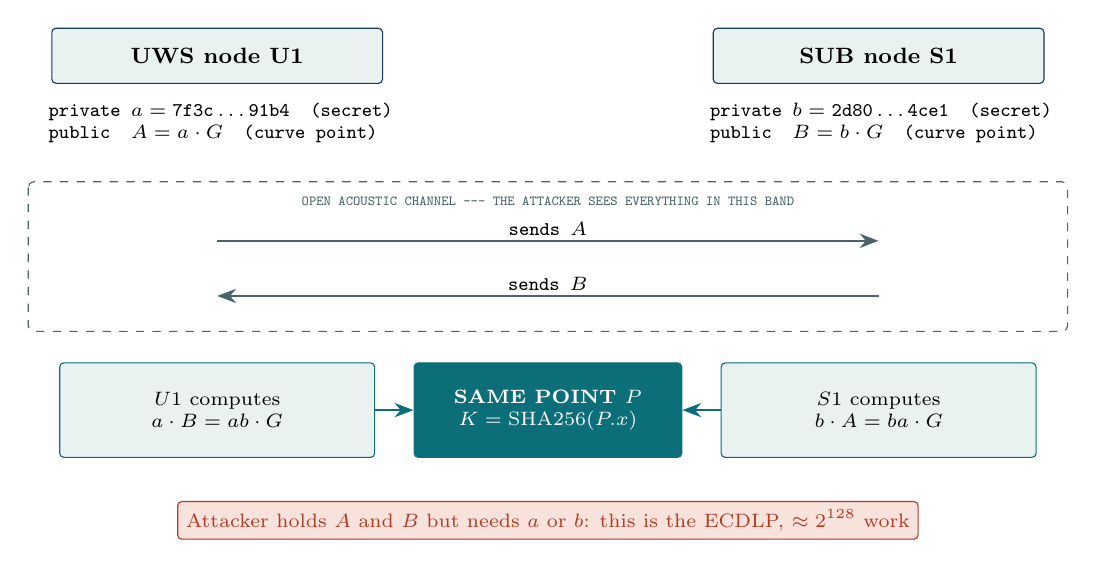
\begin{tikzpicture}[scale=1,every node/.style={transform shape}]
% headers
\node[node,minimum width=42mm,fill=mist] (u) at (-4.2,0) {UWS node U1};
\node[node,minimum width=42mm,fill=mist] (s) at ( 4.2,0) {SUB node S1};
% keys
\node[lbl,anchor=west,align=left] at (-6.4,-0.85)
  {private $a = \mathtt{7f3c\ldots91b4}$\ \ (secret)\\ public\ \ $A = a\cdot G$\ \ (curve point)};
\node[lbl,anchor=west,align=left] at ( 2.0,-0.85)
  {private $b = \mathtt{2d80\ldots4ce1}$\ \ (secret)\\ public\ \ $B = b\cdot G$\ \ (curve point)};
% open channel
\begin{scope}[on background layer]
\draw[draw=slate,dashed,rounded corners=2pt] (-6.6,-1.6) rectangle (6.6,-3.5);
\end{scope}
\node[font=\tiny\ttfamily,text=slate] at (0,-1.85)
  {OPEN ACOUSTIC CHANNEL --- THE ATTACKER SEES EVERYTHING IN THIS BAND};
\draw[flow] (-4.2,-2.35) -- node[lbl,above]{sends $A$} (4.2,-2.35);
\draw[flow] ( 4.2,-3.05) -- node[lbl,above]{sends $B$} (-4.2,-3.05);
% computation
\node[box,fill=mist,draw=teal,minimum width=40mm,minimum height=12mm] (cu) at (-4.2,-4.5)
  {$U1$ computes\\ $a\cdot B = ab\cdot G$};
\node[box,fill=mist,draw=teal,minimum width=40mm,minimum height=12mm] (cs) at ( 4.2,-4.5)
  {$S1$ computes\\ $b\cdot A = ba\cdot G$};
\node[box,fill=teal,draw=teal,text=white,minimum width=34mm,minimum height=12mm] (k) at (0,-4.5)
  {\textbf{SAME POINT $P$}\\ $K=\mathrm{SHA256}(P.x)$};
\draw[->,draw=teal,thick] (cu) -- (k);
\draw[->,draw=teal,thick] (cs) -- (k);
% attacker
\node[box,fill=palecoral,draw=coral,text=coral,minimum width=76mm] at (0,-5.9)
  {Attacker holds $A$ and $B$ but needs $a$ or $b$: this is the ECDLP, $\approx 2^{128}$ work};
\end{tikzpicture}
\caption[ECDH key agreement]{\textbf{ECDH key agreement.} Only public points cross the
channel. Each node multiplies the peer's point by its own private scalar and arrives at the
identical curve point $P$; hashing $P$'s $x$-coordinate yields a 256-bit symmetric key. The
key itself is never transmitted, so an eavesdropper who records the entire exchange still
has to solve the discrete logarithm problem.}
\label{fig:ecdh}
\end{figure}

In our simulator this is six lines of Python:

\begin{lstlisting}[style=py,caption={Key generation and ECDH shared-secret derivation
(\code{uwc\_simulation.py}, lines 109--118).}]
def gen_keys():
    pk = random.randint(1, curve.field.n - 1)   # private scalar
    return pk, pk * curve.g                     # public point

def shared(priv, pub):
    pt = priv * pub                             # ECDH: a.B on one side, b.A on the other
    return hashlib.sha256(str(pt.x).encode()).hexdigest()
\end{lstlisting}

\section{Nonces, timestamps and the replay attack}

A \textbf{nonce} is a ``number used once'': a fresh random value included in a message so
that no two runs of the protocol ever look alike. A \textbf{timestamp} records when the
message was created. Together they defeat the \textbf{replay attack}, which requires no
cryptography at all --- the adversary simply records a legitimate ciphertext and re-sends it
later. She cannot read it, but if the receiver accepts it she has impersonated a legitimate
node.

\begin{figure}[H]
\centering
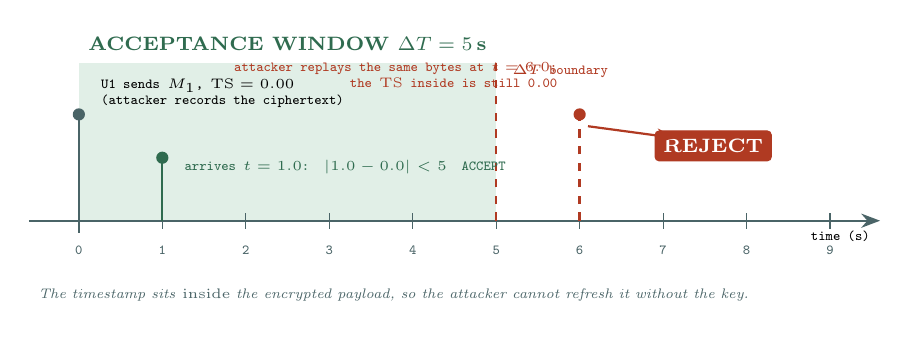
\begin{tikzpicture}[x=1.06cm,y=1cm]
% acceptance band
\fill[palekelp] (0,0.1) rectangle (5,2.1);
\node[font=\scriptsize\bfseries,text=kelp] at (2.5,2.35) {ACCEPTANCE WINDOW $\Delta T = 5$\,s};
% axis
\draw[->,thick,draw=slate] (-0.6,0.1) -- (9.6,0.1) node[below left,font=\tiny\ttfamily]{time (s)};
\foreach \x/\lb in {0/0,1/1,2/2,3/3,4/4,5/5,6/6,7/7,8/8,9/9}
  {\draw[draw=slate] (\x,0.0) -- (\x,0.2); \node[font=\tiny\ttfamily,text=slate] at (\x,-0.28) {\lb};}
\draw[thick,draw=slate] (0,-0.05) -- (0,0.25);
\draw[thick,draw=coral,dashed] (5,0.1) -- (5,2.1);
\node[font=\tiny\ttfamily,text=coral,anchor=west] at (5.08,2.0) {$\Delta T$ boundary};
% legit send
\draw[thick,draw=slate] (0,0.1) -- (0,1.45);
\fill[slate] (0,1.45) circle (2.2pt);
\node[font=\tiny\ttfamily,anchor=west,align=left] at (0.15,1.72)
  {U1 sends $M_1$, $\TS=0.00$\\ (attacker records the ciphertext)};
% legit arrival
\draw[thick,draw=kelp] (1,0.1) -- (1,0.9);
\fill[kelp] (1,0.9) circle (2.2pt);
\node[font=\tiny\ttfamily,text=kelp,anchor=west] at (1.15,0.78)
  {arrives $t=1.0$: $|1.0-0.0|<5$ \ \textbf{ACCEPT}};
% replay
\draw[very thick,draw=coral,dashed] (6,0.1) -- (6,1.45);
\fill[coral] (6,1.45) circle (2.2pt);
\node[font=\tiny\ttfamily,text=coral,anchor=east,align=right] at (5.85,1.95)
  {attacker replays the same bytes at $t=6.0$;\\ the $\TS$ inside is still 0.00};
\node[box,fill=coral,draw=coral,text=white,font=\scriptsize\bfseries] at (7.6,1.05) {REJECT};
\draw[->,thick,draw=coral] (6.1,1.3) -- (7.15,1.15);
\node[font=\tiny\itshape,text=slate,anchor=west] at (-0.6,-0.85)
  {The timestamp sits \emph{inside} the encrypted payload, so the attacker cannot refresh it without the key.};
\end{tikzpicture}
\caption[Replay defeated by the freshness window]{\textbf{Why replay fails.} The receiver
compares its own clock against the timestamp carried inside the ciphertext. Because the
adversary cannot decrypt, she cannot update that timestamp; the stale value falls outside
$\Delta T$ and the message is dropped. The nonce is the second line of defence, catching a
replay that arrives while still inside the window. $\Delta T$ is measured in seconds here,
not milliseconds, precisely because acoustic propagation is slow.}
\label{fig:replay}
\end{figure}

\section{Mutual authentication}

One-way authentication means the server proves its identity --- that is what a browser
padlock provides. \textbf{Mutual} authentication means both sides prove identity to each
other. In a sensor network both directions matter: a buoy must not accept readings from a
counterfeit sensor, and a sensor must not surrender its data to a counterfeit buoy.

The proof always has the same shape: \emph{I send you a fresh challenge that only the real
you could answer, and you return it inside something only you could have produced.}

\section{The Dolev--Yao adversary}

Formal analysis assumes the strongest realistic adversary, named after Dolev and Yao
\cite{dolevyao}. She is not an attacker sitting on one link --- she \emph{is} the network.
She may read every message, delete messages, reorder them, replay old ones, and inject
anything she can construct from what she already knows. What she cannot do is break
cryptography: without the key she cannot decrypt, and without a private key she cannot
forge. This is the \emph{perfect cryptography} assumption.

\begin{figure}[H]
\centering
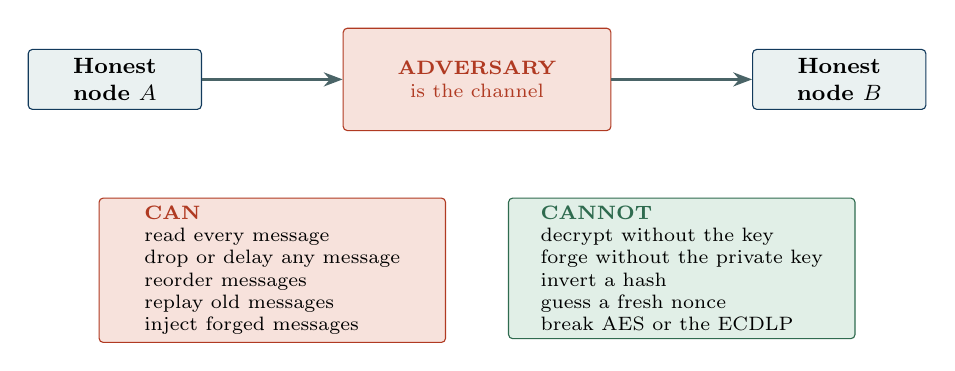
\begin{tikzpicture}
\node[node,minimum width=22mm] (a) at (-4.6,0) {Honest\\ node $A$};
\node[node,minimum width=22mm] (b) at ( 4.6,0) {Honest\\ node $B$};
\node[box,fill=palecoral,draw=coral,text=coral,minimum width=34mm,minimum height=13mm,
      font=\scriptsize\bfseries] (e) at (0,0) {ADVERSARY\\ \textnormal{\scriptsize is the channel}};
\draw[flow] (a) -- (e);
\draw[flow] (e) -- (b);
\node[box,anchor=north,align=left,minimum width=44mm,fill=palecoral,draw=coral] (can) at (-2.6,-1.5)
 {\textbf{\textcolor{coral}{CAN}}\\
  read every message\\ drop or delay any message\\ reorder messages\\
  replay old messages\\ inject forged messages};
\node[box,anchor=north,align=left,minimum width=44mm,fill=palekelp,draw=kelp] (cant) at (2.6,-1.5)
 {\textbf{\textcolor{kelp}{CANNOT}}\\
  decrypt without the key\\ forge without the private key\\
  invert a hash\\ guess a fresh nonce\\ break AES or the ECDLP};
\end{tikzpicture}
\caption[The Dolev--Yao adversary model]{\textbf{The Dolev--Yao adversary.} She controls the
entire network but not the mathematics. A protocol that survives this model has no flaw in
its \emph{message design}; any remaining weakness lies in the primitives or the
implementation. This is exactly the model Scyther checks against in
Chapter~\ref{ch:scyther}.}
\label{fig:dolevyao}
\end{figure}

\section{Notation used throughout}

\begin{table}[H]
\centering
\caption{Symbols and entities, following the base paper's Table~II.}
\label{tab:notation}
\small
\begin{tabularx}{\textwidth}{@{}L{26mm} X@{}}
\toprule
\textbf{Symbol} & \textbf{Meaning}\\
\midrule
UWS  & Underwater sensor: measures temperature, pressure, salinity, current velocity\\
SUB  & Submarine or AUV: mobile relay aggregating data from several sensors\\
B    & Surface buoy: bridges water to air, carries a GPS module\\
SAT  & Satellite: long-haul link from buoy to shore\\
BS   & Base station on land: final destination and trust anchor\\
\midrule
$\PK_i$    & Private key of entity $i$ (a secret scalar)\\
$\PU_i$    & Public key of entity $i$, $\PU_i = \PK_i \times \rho$ (a curve point)\\
$\rho$     & Generator point of the curve\\
$\ID_i$    & Identity of $i$, derived as a hash of $\PU_i$\\
$\RID_i$   & Registration identifier, $H(\ID_i \cat \PU_i \cat \PK_i)$\\
$\vartheta_i$ & Verification value, $H(\RID_i \cat \PU_i)$\\
$\Nonce_i$ & Fresh random number generated by $i$ for one run\\
$\TS_n$    & Timestamp attached to message $n$\\
$\Delta T$ & Freshness window; accept only if $|\mathrm{now} - \TS| < \Delta T$\\
$E\{\PU_j, \langle m\rangle\}$ & $m$ encrypted so only the holder of $\PK_j$ can read it\\
$D\{\PK_j, (\cdot)\}$ & Decryption with the private key of $j$\\
$\cat$     & Concatenation of fields\\
$R$        & Set of registered $\RID$s held by a node (hash table or Bloom filter)\\
$S_{i\leftrightarrow j}$ & Session established between $i$ and $j$\\
ENV        & Aggregated environmental payload $\{$Temp, Press, CurrVel, Sal$\}$\\
\bottomrule
\end{tabularx}
\end{table}

%======================================================================
\chapter{The Base Protocol}
\label{ch:proto}
%======================================================================

This chapter sets out the protocol exactly as proposed by Rupa \emph{et al.}
\cite{basepaper}: the network it assumes, its three phases, all twelve messages, and a
worked example following one real message from the seabed to the shore.

\section{Network model}

The network is a five-layer hierarchy. Data flows upward from the seabed to land, and every
adjacent pair authenticates each other before any payload moves.

\begin{itemize}
\item \textbf{UWS} --- underwater sensors on the seabed, measuring temperature (T),
      salinity (SAL), pressure (P) and current velocity (V).
\item \textbf{SUB} --- a submarine or AUV acting as a mobile hub that aggregates readings
      from several sensors.
\item \textbf{B} --- surface buoys relaying between the submarine and the satellite. Buoys
      carry GPS, so they contribute location as well as environmental data.
\item \textbf{SAT} --- satellites providing the long-distance link to shore.
\item \textbf{BS} --- the base station on land, which processes the data and acts as the
      trust anchor for revocation.
\end{itemize}

Crucially, the model builds in \textbf{redundancy}: each submarine keeps links to more than
one buoy, and each buoy can reach an alternate satellite. This is what makes the fallback
mechanism of Section~\ref{sec:fallback} possible.

\begin{figure}[H]
\centering
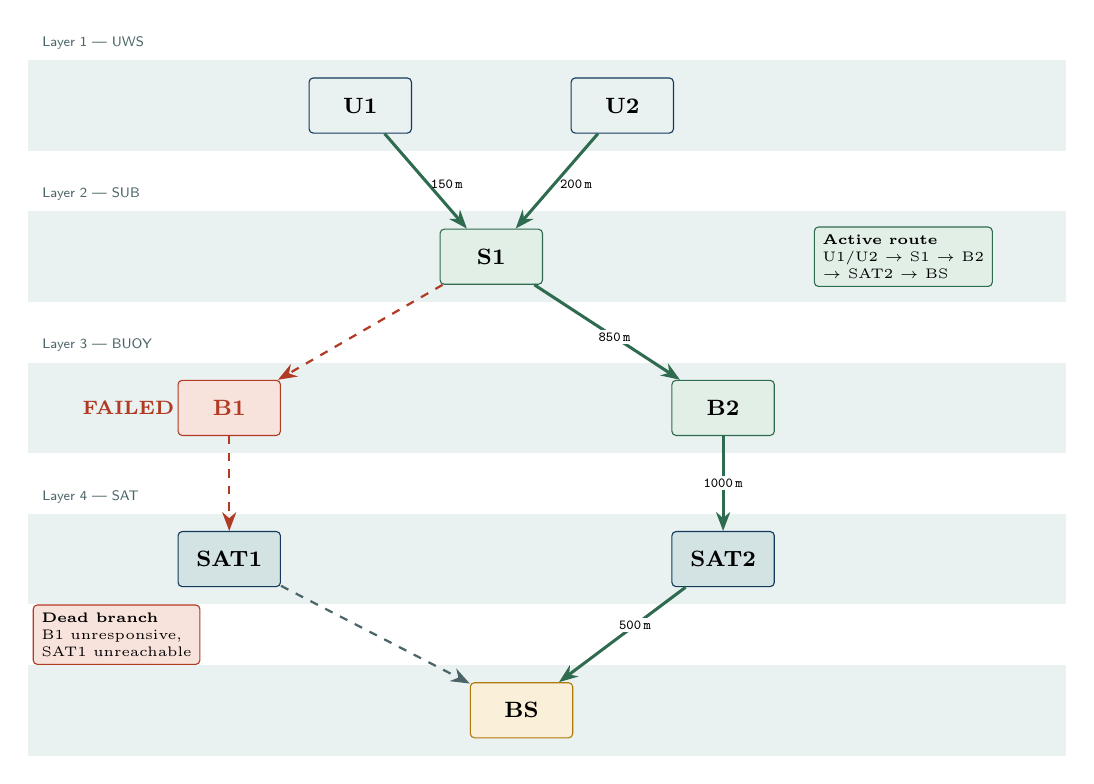
\begin{tikzpicture}[y=1.28cm,x=1.28cm]
% layer bands
\begin{scope}[on background layer]
\foreach \y/\lab in {0/{Layer 1 \textemdash\ UWS}, -1.5/{Layer 2 \textemdash\ SUB},
                     -3.0/{Layer 3 \textemdash\ BUOY}, -4.5/{Layer 4 \textemdash\ SAT},
                     -6.0/{Layer 5 \textemdash\ BS}}
  {\fill[mist] (-4.9,\y-0.45) rectangle (5.4,\y+0.45);
   \node[font=\tiny\sffamily,text=slate,anchor=west] at (-4.85,\y+0.62) {\lab};}
\end{scope}
% nodes
\node[node] (u1) at (-1.6, 0)    {U1};
\node[node] (u2) at ( 1.0, 0)    {U2};
\node[livenode] (s1) at (-0.3,-1.5) {S1};
\node[deadnode] (b1) at (-2.9,-3.0) {B1};
\node[livenode] (b2) at ( 2.0,-3.0) {B2};
\node[node,fill=mistdark] (sa1) at (-2.9,-4.5) {SAT1};
\node[node,fill=mistdark] (sa2) at ( 2.0,-4.5) {SAT2};
\node[node,fill=paleamber,draw=amber] (bs) at ( 0.0,-6.0) {BS};
% dead path
\draw[dead] (s1) -- (b1);
\draw[dead] (b1) -- (sa1);
\draw[flow,draw=slate,dashed] (sa1) -- (bs);
% active path
\draw[active] (u1) -- (s1);
\draw[active] (u2) -- (s1);
\draw[active] (s1) -- node[lblsm,fill=white,inner sep=1pt,pos=.55]{850\,m} (b2);
\draw[active] (b2) -- node[lblsm,fill=white,inner sep=1pt]{1000\,m} (sa2);
\draw[active] (sa2) -- node[lblsm,fill=white,inner sep=1pt,pos=.4]{500\,m} (bs);
\node[lblsm,anchor=east] at (-0.55,-0.78) {150\,m};
\node[lblsm,anchor=west] at (0.35,-0.78) {200\,m};
% annotations
\node[font=\scriptsize\bfseries,text=coral,anchor=east] at (-3.35,-3.0) {FAILED};
\node[box,anchor=west,align=left,fill=palekelp,draw=kelp,font=\tiny] at (2.9,-1.5)
  {\textbf{Active route}\\ U1/U2 $\to$ S1 $\to$ B2\\ $\to$ SAT2 $\to$ BS};
\node[box,anchor=west,align=left,fill=palecoral,draw=coral,font=\tiny] at (-4.85,-5.25)
  {\textbf{Dead branch}\\ B1 unresponsive,\\ SAT1 unreachable};
\end{tikzpicture}
\caption[UWC network model with fallback routing]{\textbf{The network model as we
instantiate it.} Eight nodes over five layers. Buoy B1 is forced to fail in the simulation
(dashed red), so the submarine reroutes through the pre-registered fallback buoy B2 and its
satellite SAT2 (solid green). Distances are the inter-node values used in our channel model
(Section~\ref{sec:thorp}).}
\label{fig:topology}
\end{figure}

\section{Overview of the three phases}

\begin{figure}[H]
\centering
\resizebox{\textwidth}{!}{%
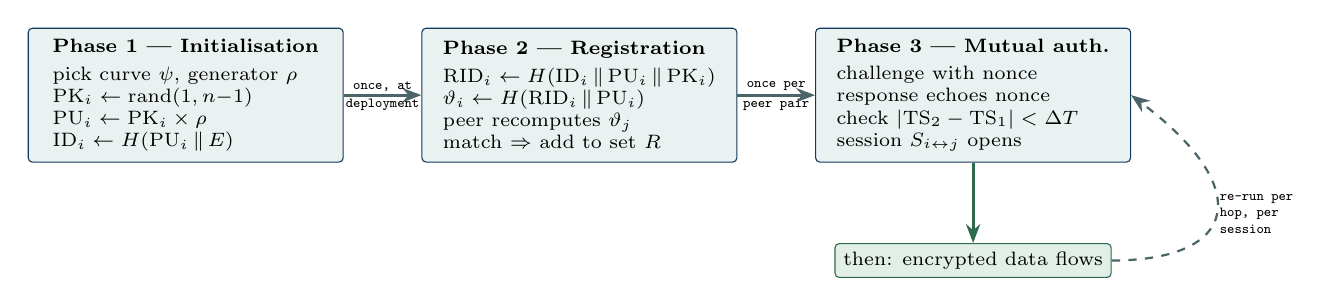
\begin{tikzpicture}[x=1cm,y=1cm]
\node[box,minimum width=40mm,minimum height=17mm,fill=mist,draw=navy,align=left] (p1) at (-4.6,0)
  {\textbf{Phase 1 \textemdash\ Initialisation}\\[2pt]
   pick curve $\psi$, generator $\rho$\\
   $\PK_i \leftarrow \mathrm{rand}(1,n{-}1)$\\
   $\PU_i \leftarrow \PK_i \times \rho$\\
   $\ID_i \leftarrow H(\PU_i \cat E)$};
\node[box,minimum width=40mm,minimum height=17mm,fill=mist,draw=navy,align=left] (p2) at (0.4,0)
  {\textbf{Phase 2 \textemdash\ Registration}\\[2pt]
   $\RID_i \leftarrow H(\ID_i\cat\PU_i\cat\PK_i)$\\
   $\vartheta_i \leftarrow H(\RID_i\cat\PU_i)$\\
   peer recomputes $\vartheta_j$\\
   match $\Rightarrow$ add to set $R$};
\node[box,minimum width=40mm,minimum height=17mm,fill=mist,draw=navy,align=left] (p3) at (5.4,0)
  {\textbf{Phase 3 \textemdash\ Mutual auth.}\\[2pt]
   challenge with nonce\\
   response echoes nonce\\
   check $|\TS_2-\TS_1|<\Delta T$\\
   session $S_{i\leftrightarrow j}$ opens};
\draw[flow,line width=1pt] (p1) -- node[lblsm,above]{once, at} node[lblsm,below]{deployment} (p2);
\draw[flow,line width=1pt] (p2) -- node[lblsm,above]{once per} node[lblsm,below]{peer pair} (p3);
\node[box,fill=palekelp,draw=kelp,minimum width=30mm,font=\scriptsize] (d) at (5.4,-2.1)
  {then: encrypted data flows};
\draw[active] (p3) -- (d);
\draw[->,draw=slate,thick,dashed] (d.east) .. controls +(1.6,0) and +(1.6,-1.2) .. (p3.east)
  node[lblsm,pos=.5,right,align=left]{re-run per\\ hop, per\\ session};
\end{tikzpicture}}
\caption[The three protocol phases]{\textbf{The three phases.} Initialisation and
registration happen once; mutual authentication runs on every hop of every session and is
where the protocol's per-message cost lives.}
\label{fig:phases}
\end{figure}

\section{Phase 1: System initialisation}

Every entity $E \in \{\mathrm{UWS, SUB, B, SAT, BS}\}$ performs six steps:

\begin{enumerate}
\item Select the pentatope elliptic curve $\psi = X^3+Y^3+Z^3+W^3+T^3 = d\,XYZWT$ over
      $\mathbb{F}_p$ for a large prime $p$ and constant $d$.
\item Choose a generator point $\rho = (X_\rho,Y_\rho,Z_\rho,W_\rho,T_\rho)$ on $\psi$ of
      large prime order $n$.
\item Generate a private key $\PK_i \in \langle 1, n-1 \rangle$ uniformly at random.
\item Compute the public key $\PU_i = \PK_i \times \rho$, where $\times$ denotes scalar
      multiplication on $\psi$.
\item Derive the identifier by hashing the public key, $\ID_i = H(\PU_i \cat E)$. Because
      $H$ is one-way and collision-resistant, an identity cannot be forged without the
      corresponding key pair.
\item Publish $M_i = (\ID_i, \PU_i)$ to the entities it must talk to.
\end{enumerate}

\begin{keybox}
\textbf{Why derive the identity from the key.} If identities were assigned arbitrarily, an
attacker could claim any identity she liked. Binding $\ID_i = H(\PU_i \cat E)$ means that to
claim an identity you must possess a public key that hashes to it --- and to \emph{use} that
identity you must hold the matching private key. Impersonation therefore reduces to
inverting a hash or solving the ECDLP. This is the mechanism behind Proposition~1 in
Section~\ref{sec:informal}.
\end{keybox}

\section{Phase 2: Registration}

Registration binds an entity to the network and gives its peers a way to detect a tampered
or duplicate registration.

\begin{enumerate}
\item $E$ computes its registration identifier and a verification value:
      \begin{equation}
      \RID_i = H(\ID_i \cat \PU_i \cat \PK_i), \qquad
      \vartheta_i = H(\RID_i \cat \PU_i)
      \end{equation}
\item $E$ sends the registration message $M_i = \{\RID_i, \PU_i, \vartheta_i\}$ to the peer
      $j$.
\item $j$ extracts $\{\RID_i, \PU_i\}$ and independently recomputes
      $\vartheta_j = H(\RID_i \cat \PU_i)$. If $\vartheta_j \neq \vartheta_i$ the message
      has been altered in transit and is rejected as \textsc{invalid}.
\item If the message is valid but $\RID_i \in R$, the registration is a duplicate and is
      refused.
\item Otherwise $\RID_i$ is added to $R$ and a session $S_{i\leftrightarrow j}$ is created.
\end{enumerate}

Note that $\RID_i$ mixes in the \emph{private} key $\PK_i$, so no other party can compute
another node's $\RID$; but because $H$ is one-way, publishing $\RID_i$ does not leak
$\PK_i$.

\subsection{Storage cost of the registration set}

The paper is careful about memory on constrained nodes. The set $R$ is a hash table or Bloom
filter giving $O(1)$ lookup, and each entity stores only the subset relevant to its own
neighbourhood --- a sensor keeps the identifiers of its submarines, not of the whole
network. With 160-bit $\RID$ values and $k$ direct peers, storage is about $20k$ bytes; for
a sensor with fewer than ten peers this is under 250 bytes. Centralised nodes such as the BS
hold the full $O(N)$ record while constrained nodes hold an $O(k)$ partial view with
$k \ll N$.

\section{Phase 3: Mutual authentication}

This is the operational core. The chain from seabed to shore is completed in twelve
messages, in a pattern that repeats identically at each of the four hops:

\begin{itemize}
\item a \textbf{challenge} carrying the initiator's identity, a fresh nonce and a timestamp;
\item an \textbf{acknowledgement} carrying the responder's identity, the \emph{same} nonce
      echoed back, and a new timestamp;
\item a \textbf{data message} carrying the payload once the session is open.
\end{itemize}

Four hops $\times$ three messages $=$ twelve. Figure~\ref{fig:msc} is the complete sequence.

\begin{figure}[H]
\centering
\resizebox{\textwidth}{!}{%
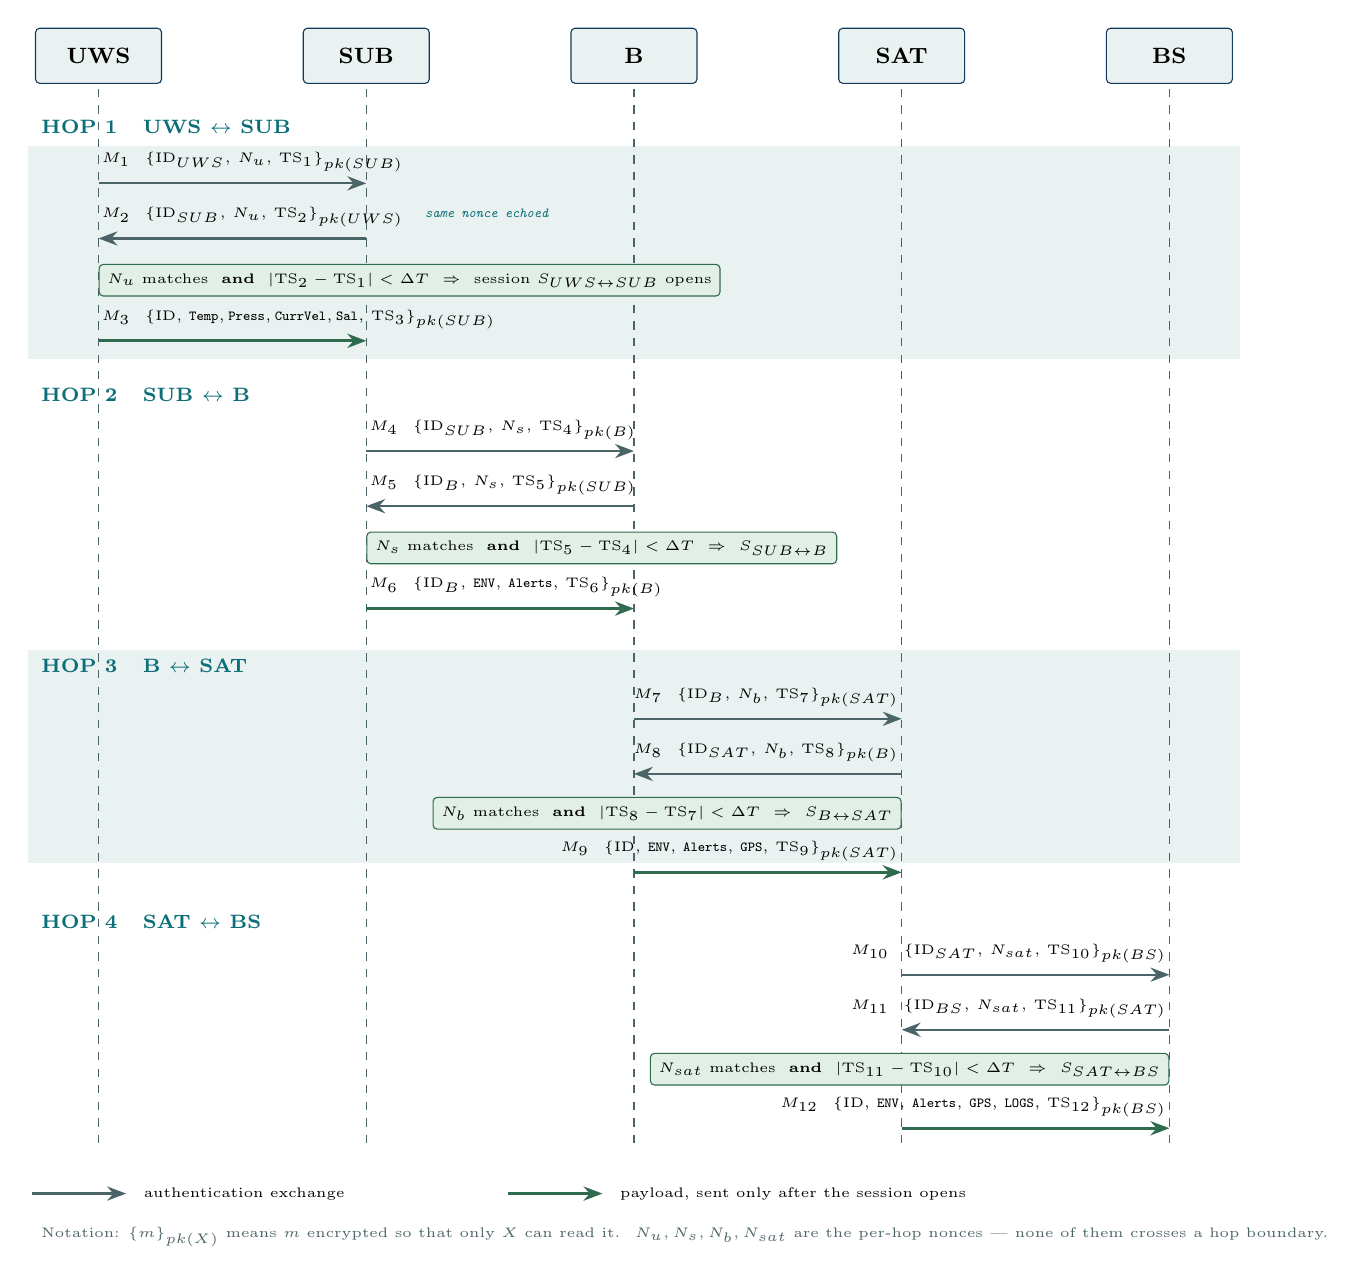
\begin{tikzpicture}[x=1cm,y=1cm,font=\footnotesize]
% lifelines
\foreach \x/\nm in {0/UWS, 3.4/SUB, 6.8/B, 10.2/SAT, 13.6/BS}
 {\node[node,minimum width=16mm] at (\x,0) {\nm};
  \draw[draw=slate,dashed] (\x,-0.42) -- (\x,-13.9);}

%================= HOP 1 : UWS <-> SUB  (labels anchored WEST at x=0)
\begin{scope}[on background layer]\fill[mist] (-0.9,-1.15) rectangle (14.5,-3.85);\end{scope}
\node[font=\scriptsize\bfseries,text=teal,anchor=west] at (-0.85,-0.9) {HOP 1 \ \ UWS $\leftrightarrow$ SUB};
\node[lblsm,anchor=west] at (0,-1.35) {$M_1$ \ $\{\ID_{UWS},\, N_u,\, \TS_1\}_{pk(SUB)}$};
\draw[flow] (0,-1.62) -- (3.4,-1.62);
\node[lblsm,anchor=west] at (0,-2.05) {$M_2$ \ $\{\ID_{SUB},\, N_u,\, \TS_2\}_{pk(UWS)}$ \ \ \textit{\textcolor{teal}{same nonce echoed}}};
\draw[flow] (3.4,-2.32) -- (0,-2.32);
\node[box,fill=palekelp,draw=kelp,font=\tiny,anchor=west] at (0,-2.85)
  {$N_u$ matches \ \textbf{and} \ $|\TS_2-\TS_1|<\Delta T$ \ $\Rightarrow$ \ session $S_{UWS\leftrightarrow SUB}$ opens};
\node[lblsm,anchor=west] at (0,-3.35) {$M_3$ \ $\{\ID,\, \mathtt{Temp},\mathtt{Press},\mathtt{CurrVel},\mathtt{Sal},\, \TS_3\}_{pk(SUB)}$};
\draw[active] (0,-3.62) -- (3.4,-3.62);

%================= HOP 2 : SUB <-> B  (labels anchored WEST at x=3.4)
\node[font=\scriptsize\bfseries,text=teal,anchor=west] at (-0.85,-4.3) {HOP 2 \ \ SUB $\leftrightarrow$ B};
\node[lblsm,anchor=west] at (3.4,-4.75) {$M_4$ \ $\{\ID_{SUB},\, N_s,\, \TS_4\}_{pk(B)}$};
\draw[flow] (3.4,-5.02) -- (6.8,-5.02);
\node[lblsm,anchor=west] at (3.4,-5.45) {$M_5$ \ $\{\ID_{B},\, N_s,\, \TS_5\}_{pk(SUB)}$};
\draw[flow] (6.8,-5.72) -- (3.4,-5.72);
\node[box,fill=palekelp,draw=kelp,font=\tiny,anchor=west] at (3.4,-6.25)
  {$N_s$ matches \ \textbf{and} \ $|\TS_5-\TS_4|<\Delta T$ \ $\Rightarrow$ \ $S_{SUB\leftrightarrow B}$};
\node[lblsm,anchor=west] at (3.4,-6.75) {$M_6$ \ $\{\ID_{B},\, \mathtt{ENV},\, \mathtt{Alerts},\, \TS_6\}_{pk(B)}$};
\draw[active] (3.4,-7.02) -- (6.8,-7.02);

%================= HOP 3 : B <-> SAT  (labels anchored EAST at x=10.2)
\begin{scope}[on background layer]\fill[mist] (-0.9,-7.55) rectangle (14.5,-10.25);\end{scope}
\node[font=\scriptsize\bfseries,text=teal,anchor=west] at (-0.85,-7.75) {HOP 3 \ \ B $\leftrightarrow$ SAT};
\node[lblsm,anchor=east] at (10.2,-8.15) {$M_7$ \ $\{\ID_{B},\, N_b,\, \TS_7\}_{pk(SAT)}$};
\draw[flow] (6.8,-8.42) -- (10.2,-8.42);
\node[lblsm,anchor=east] at (10.2,-8.85) {$M_8$ \ $\{\ID_{SAT},\, N_b,\, \TS_8\}_{pk(B)}$};
\draw[flow] (10.2,-9.12) -- (6.8,-9.12);
\node[box,fill=palekelp,draw=kelp,font=\tiny,anchor=east] at (10.2,-9.62)
  {$N_b$ matches \ \textbf{and} \ $|\TS_8-\TS_7|<\Delta T$ \ $\Rightarrow$ \ $S_{B\leftrightarrow SAT}$};
\node[lblsm,anchor=east] at (10.2,-10.1) {$M_9$ \ $\{\ID,\, \mathtt{ENV},\, \mathtt{Alerts},\, \mathtt{GPS},\, \TS_9\}_{pk(SAT)}$};
\draw[active] (6.8,-10.37) -- (10.2,-10.37);

%================= HOP 4 : SAT <-> BS  (labels anchored EAST at x=13.6)
\node[font=\scriptsize\bfseries,text=teal,anchor=west] at (-0.85,-11.0) {HOP 4 \ \ SAT $\leftrightarrow$ BS};
\node[lblsm,anchor=east] at (13.6,-11.4) {$M_{10}$ \ $\{\ID_{SAT},\, N_{sat},\, \TS_{10}\}_{pk(BS)}$};
\draw[flow] (10.2,-11.67) -- (13.6,-11.67);
\node[lblsm,anchor=east] at (13.6,-12.1) {$M_{11}$ \ $\{\ID_{BS},\, N_{sat},\, \TS_{11}\}_{pk(SAT)}$};
\draw[flow] (13.6,-12.37) -- (10.2,-12.37);
\node[box,fill=palekelp,draw=kelp,font=\tiny,anchor=east] at (13.6,-12.87)
  {$N_{sat}$ matches \ \textbf{and} \ $|\TS_{11}-\TS_{10}|<\Delta T$ \ $\Rightarrow$ \ $S_{SAT\leftrightarrow BS}$};
\node[lblsm,anchor=east] at (13.6,-13.35) {$M_{12}$ \ $\{\ID,\, \mathtt{ENV},\, \mathtt{Alerts},\, \mathtt{GPS},\, \mathtt{LOGS},\, \TS_{12}\}_{pk(BS)}$};
\draw[active] (10.2,-13.62) -- (13.6,-13.62);

%================= legend
\draw[flow] (-0.85,-14.45) -- (0.35,-14.45);
\node[font=\tiny,anchor=west] at (0.45,-14.45) {authentication exchange};
\draw[active] (5.2,-14.45) -- (6.4,-14.45);
\node[font=\tiny,anchor=west] at (6.5,-14.45) {payload, sent only after the session opens};
\node[font=\tiny,anchor=west,text=slate] at (-0.85,-15.0)
  {Notation: $\{m\}_{pk(X)}$ means $m$ encrypted so that only $X$ can read it. \ $N_u,N_s,N_b,N_{sat}$ are the per-hop nonces \textemdash\ none of them crosses a hop boundary.};
\end{tikzpicture}}
\caption[Complete twelve-message authentication chain]{\textbf{The full protocol,
$M_1$ through $M_{12}$.} Each hop repeats the same three-message pattern: challenge,
acknowledgement echoing the nonce, then payload. Sessions are established
\emph{independently} per hop --- the sensor never talks to the base station directly, and no
nonce crosses a hop boundary. The payload grows as it climbs: sensor readings at hop~1, plus
alerts at hop~2, plus GPS at hop~3, plus logistics at hop~4.}
\label{fig:msc}
\end{figure}

\subsection{Steps in words}

\begin{enumerate}[label=\textbf{M\arabic*.},leftmargin=11mm]
\item UWS $\to$ SUB. The sensor encrypts $\langle \ID_{UWS} \cat \Nonce_{UWS} \cat \TS_1
      \rangle$ under the submarine's public key. Only the submarine, holding $\PK_{SUB}$,
      can decrypt --- so a successful decryption is already evidence the message was
      intended for it.
\item SUB $\to$ UWS. The submarine replies with its own identity, \emph{the same nonce}, and
      a fresh timestamp, encrypted under the sensor's public key. Echoing the nonce is the
      proof of liveness: only a party that could decrypt $M_1$ knows what to echo.
\item Session check. UWS verifies $\Nonce^{recv}_{SUB} = \Nonce^{sent}_{UWS}$ and
      $|\TS_2 - \TS_1| < \Delta T$. Both must hold. The session $S_{UWS \leftrightarrow SUB}$
      opens, and UWS sends the sensor payload
      $\langle$Temp, Press, CurrVel, Sal$\rangle$ as $M_3$. SUB aggregates it into ENV.
\item[\textbf{M4--M6.}] The identical pattern runs between SUB and B, with SUB's nonce. At
      $M_6$ the submarine forwards ENV plus \emph{Alerts} --- notifications of jamming,
      spoofing or eavesdropping detected lower down.
\item[\textbf{M7--M9.}] The pattern runs between B and SAT. At $M_9$ the buoy adds its
      \emph{GPS} coordinates to the payload.
\item[\textbf{M10--M12.}] The pattern runs between SAT and BS. At $M_{12}$ the satellite
      adds machine and logistics updates (\emph{LOGS}), and the base station receives the
      complete record.
\end{enumerate}

\begin{keybox}
\textbf{The central design decision.} Freshness is verified \emph{per hop}. Each hop
generates its own nonce and validates its own timestamp difference. Nothing propagates
end-to-end, and there is no global session state to track. This is what makes the protocol
viable underwater: a lost packet costs one hop's retry, not a whole-chain restart, and the
1.7\,s end-to-end propagation delay never enters a freshness check.
\end{keybox}

\section{A worked example: one message end to end}
\label{sec:worked}

Abstract notation hides how little actually happens per message. Figure~\ref{fig:pipeline}
traces $M_1$ from sensor U1 to submarine S1 using the real field sizes and real value shapes
our simulator produces.

\begin{figure}[H]
\centering
\resizebox{\textwidth}{!}{%
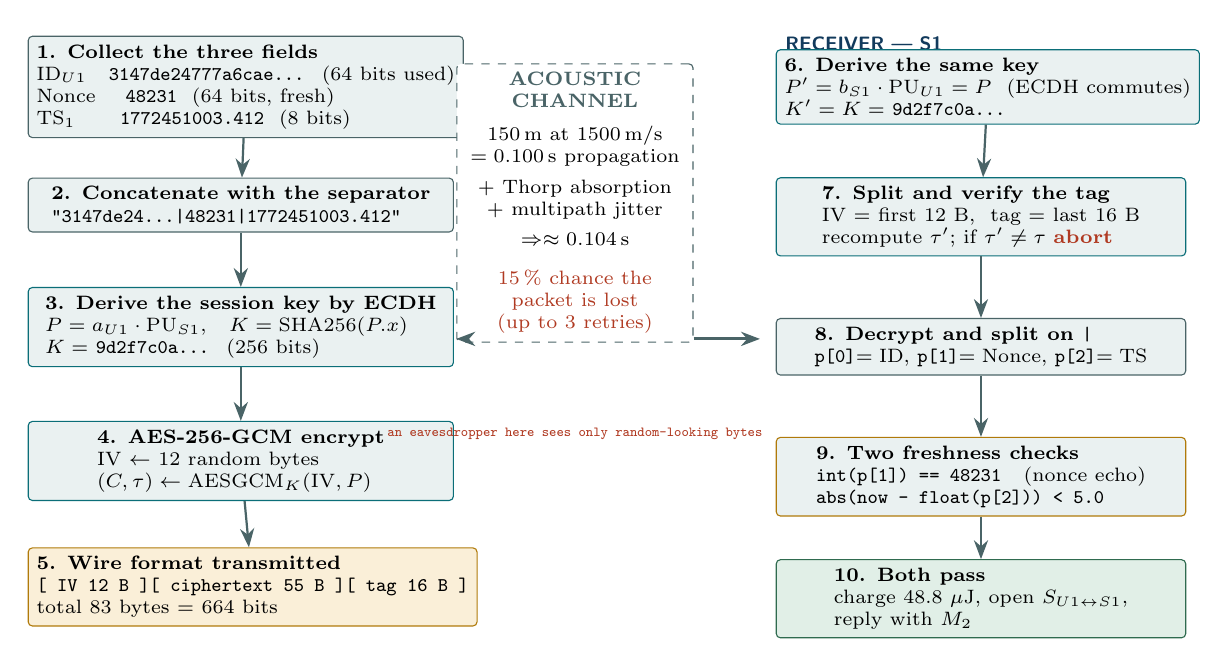
\begin{tikzpicture}[x=1cm,y=1cm,font=\scriptsize]
% ---- sender column
\node[font=\scriptsize\bfseries\sffamily,text=navy,anchor=west] at (-6.6,0.55) {SENDER \textemdash\ U1};
\node[box,anchor=west,align=left,minimum width=54mm,fill=mist] (s1) at (-6.6,0)
 {\textbf{1. Collect the three fields}\\
  $\ID_{U1}$ \ \ \texttt{3147de24777a6cae\ldots} \ (64 bits used)\\
  $\Nonce$ \ \ \ \texttt{48231} \ (64 bits, fresh)\\
  $\TS_1$ \ \ \ \ \ \texttt{1772451003.412} \ (8 bits)};
\node[box,anchor=west,align=left,minimum width=54mm,fill=mist] (s2) at (-6.6,-1.5)
 {\textbf{2. Concatenate with the separator}\\
  \texttt{"3147de24\ldots|48231|1772451003.412"}};
\node[box,anchor=west,align=left,minimum width=54mm,fill=mist,draw=teal] (s3) at (-6.6,-3.05)
 {\textbf{3. Derive the session key by ECDH}\\
  $P = a_{U1}\cdot \PU_{S1}$, \ \ $K=\mathrm{SHA256}(P.x)$\\
  $K=$ \texttt{9d2f7c0a\ldots} \ (256 bits)};
\node[box,anchor=west,align=left,minimum width=54mm,fill=mist,draw=teal] (s4) at (-6.6,-4.75)
 {\textbf{4. AES-256-GCM encrypt}\\
  IV $\leftarrow$ 12 random bytes\\
  $(C, \tau) \leftarrow \mathrm{AESGCM}_K(\mathrm{IV}, P)$};
\node[box,anchor=west,align=left,minimum width=54mm,fill=paleamber,draw=amber] (s5) at (-6.6,-6.35)
 {\textbf{5. Wire format transmitted}\\
  \texttt{[ IV 12 B ][ ciphertext 55 B ][ tag 16 B ]}\\
  total 83 bytes $=$ 664 bits};
\foreach \a/\b in {s1/s2, s2/s3, s3/s4, s4/s5} \draw[flow] (\a) -- (\b);

% ---- channel
\node[box,anchor=north,align=center,minimum width=30mm,minimum height=34mm,
      fill=white,draw=slate,dashed] (ch) at (0.35,0.3)
 {\textbf{\textcolor{slate}{ACOUSTIC}}\\ \textbf{\textcolor{slate}{CHANNEL}}\\[4pt]
  150\,m at 1500\,m/s\\ $=0.100$\,s propagation\\[3pt]
  $+$ Thorp absorption\\ $+$ multipath jitter\\[3pt]
  $\Rightarrow \approx 0.104$\,s\\[6pt]
  \textcolor{coral}{15\,\% chance the}\\ \textcolor{coral}{packet is lost}\\
  \textcolor{coral}{(up to 3 retries)}};
\draw[flow,line width=1.1pt] (-1.0,-3.2) -- (ch.west|-0,-3.2);
\draw[flow,line width=1.1pt] (ch.east|-0,-3.2) -- (2.7,-3.2);
\node[font=\tiny\ttfamily,text=coral,anchor=south] at (0.35,-4.6)
  {an eavesdropper here sees only random-looking bytes};

% ---- receiver column
\node[font=\scriptsize\bfseries\sffamily,text=navy,anchor=west] at (2.9,0.55) {RECEIVER \textemdash\ S1};
\node[box,anchor=west,align=left,minimum width=52mm,fill=mist,draw=teal] (r1) at (2.9,0)
 {\textbf{6. Derive the same key}\\
  $P' = b_{S1}\cdot \PU_{U1} = P$\ \ (ECDH commutes)\\
  $K' = K =$ \texttt{9d2f7c0a\ldots}};
\node[box,anchor=west,align=left,minimum width=52mm,fill=mist,draw=teal] (r2) at (2.9,-1.65)
 {\textbf{7. Split and verify the tag}\\
  IV $=$ first 12 B, \ tag $=$ last 16 B\\
  recompute $\tau'$; if $\tau' \neq \tau$ \textcolor{coral}{\textbf{abort}}};
\node[box,anchor=west,align=left,minimum width=52mm,fill=mist] (r3) at (2.9,-3.3)
 {\textbf{8. Decrypt and split on \texttt{|}}\\
  \texttt{p[0]}$=\ID$, \texttt{p[1]}$=\Nonce$, \texttt{p[2]}$=\TS$};
\node[box,anchor=west,align=left,minimum width=52mm,fill=mist,draw=amber] (r4) at (2.9,-4.95)
 {\textbf{9. Two freshness checks}\\
  \texttt{int(p[1]) == 48231} \ \ (nonce echo)\\
  \texttt{abs(now - float(p[2])) < 5.0}};
\node[box,anchor=west,align=left,minimum width=52mm,fill=palekelp,draw=kelp] (r5) at (2.9,-6.5)
 {\textbf{10. Both pass}\\
  charge 48.8\,\uJ, open $S_{U1\leftrightarrow S1}$,\\
  reply with $M_2$};
\foreach \a/\b in {r1/r2, r2/r3, r3/r4, r4/r5} \draw[flow] (\a) -- (\b);
\end{tikzpicture}}
\caption[One message traced through every stage]{\textbf{$M_1$ from U1 to S1, stage by
stage.} The left column is what the sender does, the right column what the receiver does,
and the centre is the physical channel. Steps~3 and~6 produce the same key without it ever
crossing the channel. Steps~4 and~7 are our AES-GCM substitution
(Section~\ref{sec:aes}); the base paper writes this stage as a public-key encryption under
$\PU_{SUB}$, which is cryptographically equivalent in effect and cheaper in practice. Note
that the tag is checked at step~7 \emph{before} any plaintext is trusted.}
\label{fig:pipeline}
\end{figure}

\subsection{Where the 2112 bits come from}

The paper's headline communication figure is 2112 bits for a complete authentication cycle.
Its accounting uses standardised field sizes: 64-bit identities, 64-bit nonces, 8-bit
timestamps, 160-bit hash outputs, and 512-bit representations for ECC points or AES keys.
Summing the fields transmitted across the login and authentication phases of all four hops
gives 2112 bits, against 3008--3216 bits for the five comparison schemes. At a nominal
modem rate of 10\,kbps, 2112 bits occupy
\begin{equation}
t_{tx} = \frac{2112 \text{ bits}}{10\,000 \text{ bits/s}} = 211\text{ ms},
\end{equation}
which is the reference line drawn on our delay plot in Chapter~\ref{ch:results}.

\section{Resilience through fallback paths}
\label{sec:fallback}

A relay in the sea is not a reliable component. Buoys are struck by shipping, drift out of
position, flood, or simply run down. The base paper's answer is \emph{dynamic reassignment
to fallback authentication peers}.

If a buoy $B_1$ stops responding, the submarine reinitiates mutual authentication with an
alternate buoy $B_2$ taken from its neighbour list. Likewise a buoy can route to a secondary
satellite when the primary fails or is delayed. The essential detail is that these fallback
entities are \textbf{pre-registered during system initialisation} and held in a trusted
cache. Rerouting therefore does not require a new registration exchange --- the public keys
and registration identifiers are already known --- and the same nonce-freshness and
timestamp bounds validate the rerouted session as would validate an original one.

\begin{figure}[H]
\centering
\resizebox{0.96\textwidth}{!}{%
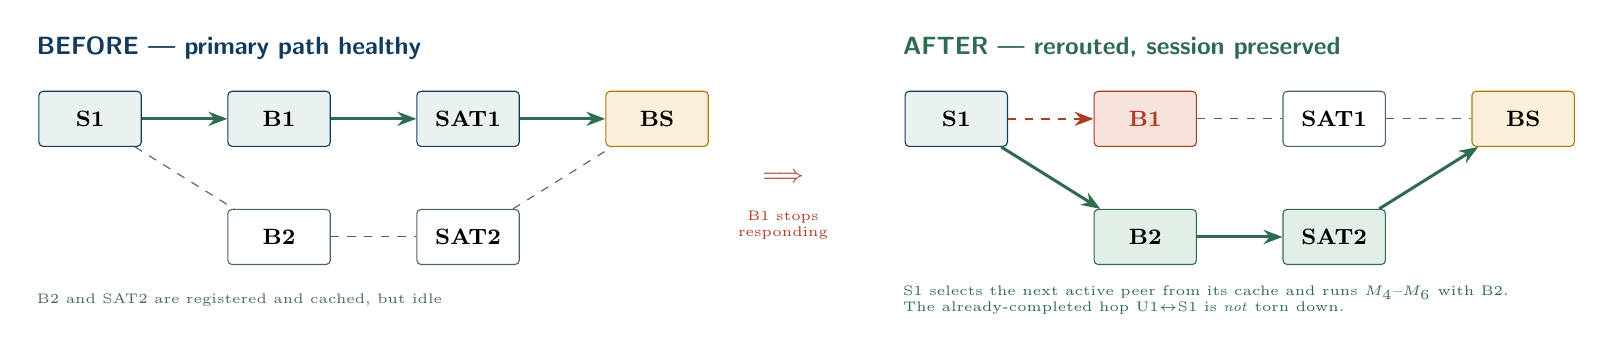
\begin{tikzpicture}[x=1cm,y=1cm,font=\scriptsize]
%---------------- BEFORE
\node[font=\small\bfseries\sffamily,text=navy,anchor=west] at (0,1.5) {BEFORE \textemdash\ primary path healthy};
\node[node] (a1) at (0.8,0.6) {S1};
\node[node] (a2) at (3.2,0.6) {B1};
\node[node] (a3) at (5.6,0.6) {SAT1};
\node[node,fill=paleamber,draw=amber] (a4) at (8.0,0.6) {BS};
\node[node,fill=white,draw=slate] (a5) at (3.2,-0.9) {B2};
\node[node,fill=white,draw=slate] (a6) at (5.6,-0.9) {SAT2};
\draw[active] (a1) -- (a2); \draw[active] (a2) -- (a3); \draw[active] (a3) -- (a4);
\draw[draw=slate,dashed] (a1) -- (a5); \draw[draw=slate,dashed] (a5) -- (a6);
\draw[draw=slate,dashed] (a6) -- (a4);
\node[font=\tiny,text=slate,anchor=west] at (0.0,-1.7)
  {B2 and SAT2 are registered and cached, but idle};
%---------------- arrow
\node[font=\small\bfseries,text=coral] at (9.6,-0.15) {$\Longrightarrow$};
\node[font=\tiny,text=coral,align=center] at (9.6,-0.75) {B1 stops\\ responding};
%---------------- AFTER
\node[font=\small\bfseries\sffamily,text=kelp,anchor=west] at (11.0,1.5) {AFTER \textemdash\ rerouted, session preserved};
\node[node] (b1) at (11.8,0.6) {S1};
\node[deadnode] (b2) at (14.2,0.6) {B1};
\node[node,fill=white,draw=slate] (b3) at (16.6,0.6) {SAT1};
\node[node,fill=paleamber,draw=amber] (b4) at (19.0,0.6) {BS};
\node[livenode] (b5) at (14.2,-0.9) {B2};
\node[livenode] (b6) at (16.6,-0.9) {SAT2};
\draw[dead] (b1) -- (b2);
\draw[draw=slate,dashed] (b2) -- (b3); \draw[draw=slate,dashed] (b3) -- (b4);
\draw[active] (b1) -- (b5); \draw[active] (b5) -- (b6); \draw[active] (b6) -- (b4);
\node[font=\tiny,text=kelp,anchor=west,align=left] at (11.0,-1.7)
  {S1 selects the next active peer from its cache and runs $M_4$--$M_6$ with B2.\\
   The already-completed hop U1$\leftrightarrow$S1 is \emph{not} torn down.};
\end{tikzpicture}}
\caption[Dynamic fallback rerouting]{\textbf{Fallback in action.} Because $B_2$ was
registered at initialisation, the submarine can authenticate with it immediately; only the
three messages of the failed hop are repeated. Nothing upstream is affected, which is the
direct benefit of authenticating per hop rather than end to end.}
\label{fig:fallback}
\end{figure}

The paper reports that a new session can be established in under 1\,ms thanks to the
lightweight cryptographic operations and pre-distributed public keys, so a node that drifts
into a new submarine's range can simply re-run $M_1$--$M_3$ rather than waiting on a
recovery procedure. Ongoing sessions remain valid as long as latency stays within
$\Delta T$ and loss stays below threshold.

\section{Long-term key management}

Three provisions in the paper address cryptographic sustainability over a deployment
lifetime.

\begin{enumerate}
\item \textbf{Secure private-key storage.} Private keys are held in tamper-resistant
      hardware --- a secure element such as the Microchip ATECC608A, or a TPM --- where cost
      and power allow. Where they do not, the paper falls back on firmware-level obfuscation
      and memory isolation to raise the cost of physical extraction.
\item \textbf{Key revocation.} The base station periodically issues a signed revocation
      list naming compromised or expired nodes. It is broadcast to the network, and every
      entity checks incoming messages against it before initiating or answering an
      authentication. The list itself is authenticated with a management key held by all
      trusted nodes.
\item \textbf{Initial public-key distribution.} At deployment each node uploads its public
      key to the base station over a trusted link --- a physical interface, or a short-range
      line-of-sight acoustic channel. The key is bound to the identity by
      \begin{equation}
      \ID_i = H(\PU_i \cat E \cat \mathrm{DeviceSerial})
      \end{equation}
      which prevents identity spoofing, and the keys are then disseminated to the other
      entities so mutual authentication can proceed.
\end{enumerate}

%======================================================================
\chapter{Security Analysis and Performance in the Base Paper}
\label{ch:basesec}
%======================================================================

Having set out what the protocol \emph{does}, this chapter covers the paper's argument that
it is \emph{secure}, and its accounting of what it costs. Three separate arguments are made:
a formal proof in BAN logic, a set of informal propositions, and machine verification with
Scyther.

\section{Threat model}

The paper assumes an adversary capable of:

\begin{itemize}
\item \textbf{Passive eavesdropping} --- recording everything on the channel.
\item \textbf{Active impersonation} --- claiming to be a legitimate node.
\item \textbf{Replay} --- retransmitting captured messages.
\item \textbf{Delay injection} --- deliberately slowing packets to push a legitimate
      exchange outside its timestamp window, causing desynchronisation.
\item \textbf{Physical tampering} --- compromising a subset of nodes and extracting their
      stored credentials.
\end{itemize}

The four defences claimed against these are: unique non-reusable nonces with adaptive
timestamp validation; asymmetric encryption with secure key derivation; tamper-resistant
storage with hierarchical credential management; and revocation combined with dynamic
fallback paths.

\section{Formal analysis with BAN logic}

BAN logic \cite{ban} is a formal system for reasoning about \emph{belief} in authentication
protocols. Rather than modelling bits, it models what each participant is entitled to
conclude after seeing a message. It is a proof technique, not a tool: you write down what
each party initially believes, apply inference rules to each message, and check whether the
desired beliefs follow.

\subsection{Notation}

For entities $\varepsilon, \phi$ and messages $M_\varepsilon, M_\phi$:

\begin{table}[H]
\centering
\small
\caption{BAN logic notation used in the base paper's proof.}
\label{tab:ban-not}
\begin{tabularx}{\textwidth}{@{}L{30mm} X@{}}
\toprule
\textbf{Notation} & \textbf{Reading}\\
\midrule
$\prec M_\varepsilon \succ$ & Message $M_\varepsilon$ is \emph{fresh}\\
$\varepsilon \Lleftarrow M_\varepsilon$ & $\varepsilon$ \emph{sees} the statement\\
$\varepsilon \Rightarrow M_\varepsilon$ & $\varepsilon$ has \emph{jurisdiction} over the statement\\
$\varepsilon \gg M_\varepsilon$ & $\varepsilon$ \emph{believes} the statement\\
$\varepsilon \sim M_\varepsilon$ & $\varepsilon$ \emph{once said} the statement\\
$\{M_\varepsilon\}_{\PU_\varepsilon}$ & Encrypted under $\varepsilon$'s public key\\
$\phi \xLeftrightarrow{\PU_\varepsilon} \varepsilon$ & The two communicate securely using $\PU_\varepsilon$\\
\bottomrule
\end{tabularx}
\end{table}

\subsection{Inference rules}

\begin{table}[H]
\centering
\small
\caption{The five BAN rules applied in the proof.}
\label{tab:ban-rules}
\begin{tabularx}{\textwidth}{@{}L{10mm} L{40mm} X@{}}
\toprule
& \textbf{Rule} & \textbf{Plain reading}\\
\midrule
R1 & Message-meaning &
  If I believe we share a key and I see a message encrypted under it, then I believe you
  sent that message.\\
R2 & Nonce-verification &
  If I believe the message is fresh and that you sent it, then I believe you currently
  believe it (not that you said it long ago).\\
R3 & Jurisdiction &
  If I believe you are authoritative over a statement and that you believe it, then I
  believe it.\\
R4 & Freshness &
  If any part of a message is fresh, the whole message is fresh.\\
R5 & Belief &
  If I believe you believe a compound message, I believe you believe each part.\\
\bottomrule
\end{tabularx}
\end{table}

\subsection{Goals, assumptions and the derivation}

Eight goals are stated, one per direction of each of the four hops:
\begin{align}
\Omega_1&: \mathrm{UWS} \gg (\mathrm{UWS} \xLeftrightarrow{\PU_{SUB}} \mathrm{SUB}) &
\Omega_2&: \mathrm{SUB} \gg (\mathrm{UWS} \xLeftrightarrow{\PU_{UWS}} \mathrm{SUB}) \notag\\
\Omega_3&: \mathrm{SUB} \gg (\mathrm{SUB} \xLeftrightarrow{\PU_{B}} \mathrm{B}) &
\Omega_4&: \mathrm{B} \gg (\mathrm{SUB} \xLeftrightarrow{\PU_{SUB}} \mathrm{B}) \notag\\
\Omega_5&: \mathrm{B} \gg (\mathrm{B} \xLeftrightarrow{\PU_{SAT}} \mathrm{SAT}) &
\Omega_6&: \mathrm{SAT} \gg (\mathrm{B} \xLeftrightarrow{\PU_{B}} \mathrm{SAT}) \notag\\
\Omega_7&: \mathrm{SAT} \gg (\mathrm{SAT} \xLeftrightarrow{\PU_{BS}} \mathrm{BS}) &
\Omega_8&: \mathrm{BS} \gg (\mathrm{SAT} \xLeftrightarrow{\PU_{SAT}} \mathrm{BS}) \notag
\end{align}

The initial assumptions are that every entity believes its own nonces and timestamps are
fresh ($A_1, A_2$), that each entity has jurisdiction over its own identity ($A_3$), and
that public keys are correctly distributed ($A_4$).

The derivation then runs for thirty steps. Figure~\ref{fig:ban} shows the first hop, which
is representative --- the other three hops repeat the identical five-step shape.

\begin{figure}[H]
\centering
\resizebox{\textwidth}{!}{%
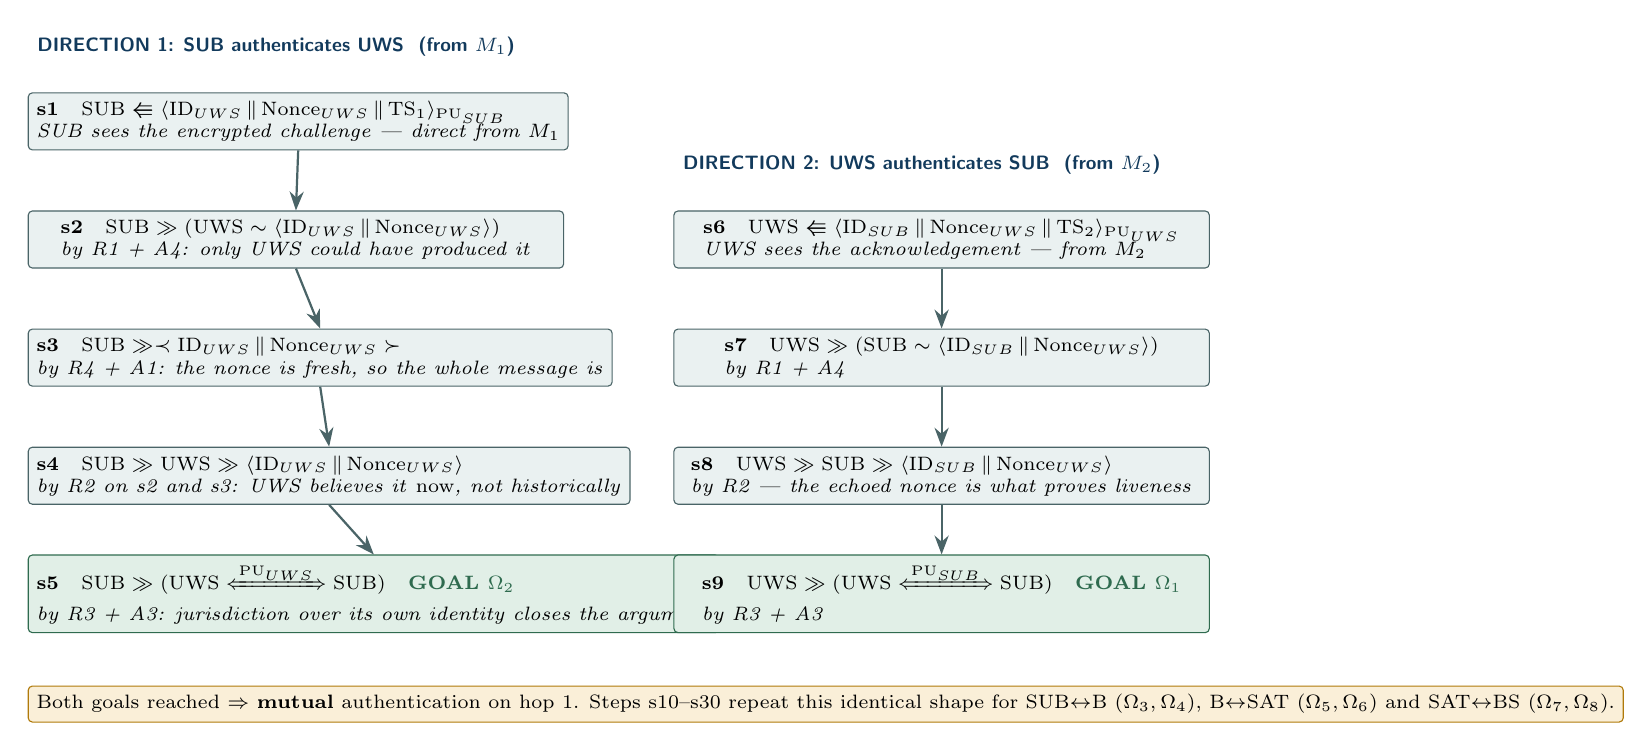
\begin{tikzpicture}[x=1cm,y=1cm,font=\footnotesize]
\node[box,anchor=west,align=left,minimum width=68mm,fill=mist] (s1) at (0,0)
 {\textbf{s1} \ \ $\mathrm{SUB} \Lleftarrow \langle \ID_{UWS}\cat\Nonce_{UWS}\cat\TS_1\rangle_{\PU_{SUB}}$\\
  \textit{\scriptsize SUB sees the encrypted challenge \textemdash\ direct from $M_1$}};
\node[box,anchor=west,align=left,minimum width=68mm,fill=mist] (s2) at (0,-1.5)
 {\textbf{s2} \ \ $\mathrm{SUB} \gg (\mathrm{UWS} \sim \langle \ID_{UWS}\cat\Nonce_{UWS}\rangle)$\\
  \textit{\scriptsize by R1 + A4: only UWS could have produced it}};
\node[box,anchor=west,align=left,minimum width=68mm,fill=mist] (s3) at (0,-3.0)
 {\textbf{s3} \ \ $\mathrm{SUB} \gg \prec \ID_{UWS}\cat\Nonce_{UWS} \succ$\\
  \textit{\scriptsize by R4 + A1: the nonce is fresh, so the whole message is}};
\node[box,anchor=west,align=left,minimum width=68mm,fill=mist] (s4) at (0,-4.5)
 {\textbf{s4} \ \ $\mathrm{SUB} \gg \mathrm{UWS} \gg \langle \ID_{UWS}\cat\Nonce_{UWS}\rangle$\\
  \textit{\scriptsize by R2 on s2 and s3: UWS believes it \emph{now}, not historically}};
\node[box,anchor=west,align=left,minimum width=68mm,fill=palekelp,draw=kelp] (s5) at (0,-6.0)
 {\textbf{s5} \ \ $\mathrm{SUB} \gg (\mathrm{UWS} \xLeftrightarrow{\PU_{UWS}} \mathrm{SUB})$
  \ \ \textcolor{kelp}{\textbf{GOAL $\Omega_2$}}\\
  \textit{\scriptsize by R3 + A3: jurisdiction over its own identity closes the argument}};
\foreach \a/\b in {s1/s2,s2/s3,s3/s4,s4/s5} \draw[flow] (\a.south) -- (\b.north);
% right column: the mirror direction
\node[box,anchor=west,align=left,minimum width=68mm,fill=mist] (t1) at (8.2,-1.5)
 {\textbf{s6} \ \ $\mathrm{UWS} \Lleftarrow \langle \ID_{SUB}\cat\Nonce_{UWS}\cat\TS_2\rangle_{\PU_{UWS}}$\\
  \textit{\scriptsize UWS sees the acknowledgement \textemdash\ from $M_2$}};
\node[box,anchor=west,align=left,minimum width=68mm,fill=mist] (t2) at (8.2,-3.0)
 {\textbf{s7} \ \ $\mathrm{UWS} \gg (\mathrm{SUB} \sim \langle \ID_{SUB}\cat\Nonce_{UWS}\rangle)$\\
  \textit{\scriptsize by R1 + A4}};
\node[box,anchor=west,align=left,minimum width=68mm,fill=mist] (t3) at (8.2,-4.5)
 {\textbf{s8} \ \ $\mathrm{UWS} \gg \mathrm{SUB} \gg \langle \ID_{SUB}\cat\Nonce_{UWS}\rangle$\\
  \textit{\scriptsize by R2 \textemdash\ the echoed nonce is what proves liveness}};
\node[box,anchor=west,align=left,minimum width=68mm,fill=palekelp,draw=kelp] (t4) at (8.2,-6.0)
 {\textbf{s9} \ \ $\mathrm{UWS} \gg (\mathrm{UWS} \xLeftrightarrow{\PU_{SUB}} \mathrm{SUB})$
  \ \ \textcolor{kelp}{\textbf{GOAL $\Omega_1$}}\\
  \textit{\scriptsize by R3 + A3}};
\foreach \a/\b in {t1/t2,t2/t3,t3/t4} \draw[flow] (\a.south) -- (\b.north);
\node[font=\scriptsize\bfseries\sffamily,text=navy,anchor=west] at (0,0.95)
  {DIRECTION 1: SUB authenticates UWS \ (from $M_1$)};
\node[font=\scriptsize\bfseries\sffamily,text=navy,anchor=west] at (8.2,-0.55)
  {DIRECTION 2: UWS authenticates SUB \ (from $M_2$)};
\node[box,anchor=west,fill=paleamber,draw=amber,align=left,minimum width=150mm,font=\scriptsize] at (0,-7.4)
 {Both goals reached $\Rightarrow$ \textbf{mutual} authentication on hop 1. Steps s10--s30
  repeat this identical shape for SUB$\leftrightarrow$B ($\Omega_3,\Omega_4$),
  B$\leftrightarrow$SAT ($\Omega_5,\Omega_6$) and SAT$\leftrightarrow$BS ($\Omega_7,\Omega_8$).};
\end{tikzpicture}}
\caption[BAN logic derivation for hop 1]{\textbf{The BAN derivation, hop 1.} The left column
is the challenge direction, the right the acknowledgement direction. Reaching both goals is
what makes the authentication \emph{mutual}. The critical step is s4/s8, where the freshness
of the nonce upgrades ``$\phi$ once said this'' into ``$\phi$ believes this now'' ---
without freshness, a replayed message would satisfy the earlier steps.}
\label{fig:ban}
\end{figure}

\section{Informal security propositions}
\label{sec:informal}

The paper supplements the BAN proof with five propositions.

\begin{table}[H]
\centering
\caption{The paper's five security propositions and the mechanism behind each.}
\label{tab:props}
\small
\begin{tabularx}{\textwidth}{@{}L{8mm} L{34mm} X@{}}
\toprule
& \textbf{Claim} & \textbf{Mechanism}\\
\midrule
P1 & No identity spoofing &
  Each identity is bound to a key pair and validated by signature at registration;
  $\mathrm{Verify}(\mathrm{Sig}(\ID_i,\mathrm{SK}_i),\mathrm{PK}_i)$ must return true.
  Forging an identity means forging a signature.\\
\addlinespace[2pt]
P2 & Replay resistance &
  The receiver checks $N_i \notin \mathrm{UsedNonces}$ \emph{and}
  $|\mathrm{now}-\TS_i| \le \Delta T$. The paper further proposes an \emph{adaptive}
  $\Delta T$: each node keeps a rolling average of recent inter-node delays and adjusts the
  window, so legitimate variation is tolerated while stale injection is still caught.\\
\addlinespace[2pt]
P3 & No man-in-the-middle &
  Messages are encrypted under the recipient's public key. Only the holder of the matching
  private key can decrypt or meaningfully alter them.\\
\addlinespace[2pt]
P4 & Secure key establishment &
  $K_{ij} = \mathrm{DH}(\mathrm{PK}_i,\mathrm{SK}_j) = \mathrm{DH}(\mathrm{PK}_j,\mathrm{SK}_i)$.
  Only the two legitimate parties can compute it. Bounded $\Delta T$ per hop additionally
  causes a delay-injection attempt to abort the session.\\
\addlinespace[2pt]
P5 & Resists stolen-verifier and ephemeral-secret-leakage attacks &
  Long-term private keys authenticate session establishment only; session keys are
  ephemeral, derived from fresh nonces and timestamps, and never stored. Compromising a node
  therefore yields neither past nor future session keys --- this is forward secrecy in
  effect. The registration set is periodically checked against the BS's revocation list.\\
\bottomrule
\end{tabularx}
\end{table}

\section{Machine verification with Scyther}

Scyther \cite{scyther} is an automated model checker for security protocols developed by
Cas Cremers. You describe the protocol in SPDL (Security Protocol Description Language),
state the properties you want, and the tool searches exhaustively for a trace in which a
Dolev--Yao adversary violates one. If no such trace exists within the bound, it reports a
proof of correctness; if one does, it draws the attack.

The four properties checked are:

\begin{table}[H]
\centering
\caption{Scyther claim types and what each rules out.}
\label{tab:claims}
\small
\begin{tabularx}{\textwidth}{@{}L{24mm} X L{42mm}@{}}
\toprule
\textbf{Claim} & \textbf{Guarantee} & \textbf{Attack it rules out}\\
\midrule
\texttt{Secret} & The named value is never learned by the adversary:
  $\forall \mathcal{A},\ \Pr[\mathcal{A}(S)=S] \le \theta$ &
  Eavesdropping, key recovery\\
\texttt{Alive} & The claimed peer actually executed the protocol &
  Talking to a ghost\\
\texttt{Weakagree} & If $\varepsilon_A$ believes it ran with $\varepsilon_B$, then
  $\varepsilon_B$ really did run with $\varepsilon_A$:
  $P(\varepsilon_A,\varepsilon_B) \Rightarrow \exists P(\varepsilon_B,\varepsilon_A)$ &
  Man-in-the-middle, impersonation\\
\texttt{Niagree} / \texttt{Nisynch} & Both parties agree on all exchanged values, in a
  causally ordered sequence: a message received at $t_r$ was sent at $t_s \le t_r$ &
  Replay, message reordering, value substitution\\
\bottomrule
\end{tabularx}
\end{table}

The paper reports that all entities passed, configured for five roles with up to five
concurrent sessions each, across more than sixty test cases, with no attacks found. Its
Fig.~6 shows the tool output. The paper does not publish its SPDL source; our own
reconstruction, and the restructuring it needed, is the subject of Chapter~\ref{ch:scyther}.

\section{Performance in the base paper}

\subsection{Experimental setup}

The paper's evaluation uses a custom Python 3.10 simulator on Ubuntu 22.04, Intel Core
i7-11800H, 32\,GB RAM. The modelled network is a hierarchical tree of 10 to 200 nodes over 2
to 5 depth levels, with acoustic links at a nominal 10\,kbps, inter-node distances of 100 to
1000\,m and sound speed 1500\,m/s. Message fields are standardised at 64-bit identities,
64-bit nonces, 8-bit timestamps, 160-bit hashes and 512-bit ECC-point or AES-key
representations.

\subsection{Communication cost}

\begin{table}[H]
\centering
\caption[Communication cost comparison]{Communication cost per full authentication cycle,
in bits (base paper, Table~IV). ``Ref [21]--[25]'' are the scheme identifiers used in the
base paper's own comparison, and are \emph{not} the reference numbers of this report.}
\label{tab:comm}
\small
\begin{tabular}{@{}l r r r r r l@{}}
\toprule
\textbf{Protocol} & \textbf{Entity 1} & \textbf{Entity 2} & \textbf{Entity 3} &
\textbf{Entity 4} & \textbf{Total} & \textbf{vs proposed}\\
\midrule
Ref [21] & 896  & 768 & 512 & 832 & 3008 & $+42\,\%$\\
Ref [22] & 1024 & 832 & 512 & 832 & 3200 & $+52\,\%$\\
Ref [23] & 960  & 800 & 544 & 832 & 3136 & $+49\,\%$\\
Ref [24] & 912  & 784 & 512 & 832 & 3040 & $+44\,\%$\\
Ref [25] & 1008 & 848 & 528 & 832 & 3216 & $+52\,\%$\\
\midrule
\textbf{Proposed} & \textbf{640} & \textbf{512} & \textbf{320} & \textbf{640} &
\textbf{2112} & \textbf{baseline}\\
\bottomrule
\end{tabular}
\end{table}

The percentages are relative to the proposed scheme as denominator; for example
$(3008-2112)/2112 = 42\,\%$.

\subsection{Computational cost}

\begin{table}[H]
\centering
\caption[Computational cost comparison]{Computational cost per entity in milliseconds
(base paper, Table~V). $T_{exp}$ exponentiation, $T_{ecm}$ elliptic-curve multiplication,
$T_h$ hash, $T_{pair}$ bilinear pairing.}
\label{tab:comp}
\small
\begin{tabularx}{\textwidth}{@{}l r r X@{}}
\toprule
\textbf{Protocol} & \textbf{UWS / BS} & \textbf{SUB / SAT} & \textbf{Operations}\\
\midrule
Ref [21] & 0.536  & 0.800  & 2 exp $+$ 6 hash\\
Ref [22] & 19.70  & 25.000 & 3 ECM $+$ 4 ECM $+$ pairings\\
Ref [23] & 75.88  & 90.000 & 3 ECM $+$ 2 pairings\\
Ref [24] & 2.352  & 2.900  & 1 ECM $+$ 4 hash\\
Ref [25] & 1.245  & 1.600  & 1 ECM $+$ 3 hash\\
\midrule
\textbf{Proposed} & \textbf{0.400} & \textbf{0.500} &
\textbf{1 ECC $+$ 2 hash $+$ 4 AES}\\
\bottomrule
\end{tabularx}
\end{table}

The saving comes from eliminating bilinear pairings and multiple exponentiations --- the two
operations that dominate cost in the older schemes --- and replacing them with one optimised
ECC operation plus cheap symmetric work. Against Ref~[23] this is a $189\times$ improvement.

\subsection{Energy per authentication cycle}

The paper's energy accounting uses published ARM Cortex-M4 / Cortex-A53 benchmarks:
one ECC operation $\approx 24\,\mu$J, one hash $\approx 6\,\mu$J, one AES-128
encryption or decryption $\approx 3.2\,\mu$J. A single entity performs one ECC operation,
two hashes, and two encryptions plus two decryptions:

\begin{equation}
E_{cycle} = \underbrace{24}_{\text{ECC}}
          + \underbrace{2 \times 6}_{\text{hash}}
          + \underbrace{(2+2) \times 3.2}_{\text{AES}}
          = 24 + 12 + 12.8 = 48.8\ \mu\mathrm{J}
\label{eq:energy}
\end{equation}

\begin{table}[H]
\centering
\caption{Energy per authentication cycle against prior schemes.}
\label{tab:energy}
\small
\begin{tabular}{@{}l r l@{}}
\toprule
\textbf{Protocol} & \textbf{Energy} & \textbf{Relative}\\
\midrule
Ref [22] & $\approx 2300\ \mu$J & $47\times$ more\\
Ref [23] & $\approx 8900\ \mu$J & $182\times$ more\\
Ref [24] & $\approx 280\ \mu$J  & $5.7\times$ more\\
\midrule
\textbf{Proposed} & $\bm{48.8\ \mu}$\textbf{J} & \textbf{baseline}\\
\bottomrule
\end{tabular}
\end{table}

At 48.8\,\uJ{} --- under 0.05\,mJ --- a node with a 1000\,mAh cell at 3.3\,V
(3.3\,J $=3.3\times10^{6}$\,\uJ) could in principle perform about 67\,000 authentication
cycles on cryptography alone. Chapter~\ref{ch:results} shows what happens once transmission
and reception energy are added, which is where the real budget goes.

%======================================================================
\chapter{Our Implementation}
\label{ch:impl}
%======================================================================

The base paper specifies a protocol but publishes no code. This chapter describes what we
built, how it is organised, and --- candidly --- what was wrong with our first version. The
corrections are the subject of Chapter~\ref{ch:improve}.

\section{Deliverables}

\begin{table}[H]
\centering
\caption{Repository contents.}
\label{tab:repo}
\small
\begin{tabularx}{\textwidth}{@{}L{46mm} X@{}}
\toprule
\textbf{File} & \textbf{Purpose}\\
\midrule
\code{uwc\_simulation.py} & The simulator: 406 lines. ECC key generation, registration,
  four-hop authentication with fallback, AES-GCM, the Thorp channel, loss and
  retransmission, battery tracking, mobility, anomaly detection, and all seven plots.\\
\code{uwc\_protocol.spdl} & Scyther model: four protocols, eight roles, 32 claims.\\
\code{requirements.txt} & \code{tinyec}, \code{cryptography}, \code{networkx},
  \code{matplotlib}, \code{numpy}, \code{scipy}.\\
\code{scyther/} & The bundled Scyther 1.3.0 distribution, so verification is reproducible
  without a separate download.\\
\code{launch\_scyther\_gui.bat} & One-click launcher for the bundled GUI.\\
\code{output/} & The seven generated plots plus the GUI verification screenshot.\\
\bottomrule
\end{tabularx}
\end{table}

\section{Architecture of the simulator}

\begin{figure}[H]
\centering
\resizebox{0.98\textwidth}{!}{%
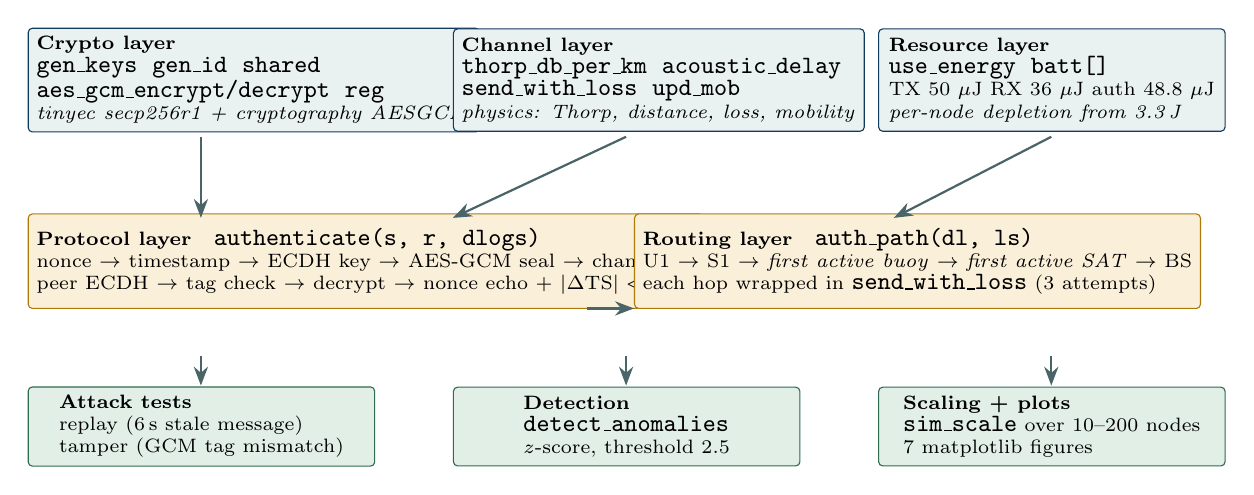
\begin{tikzpicture}[x=1cm,y=1cm,font=\scriptsize]
% layers
\node[box,anchor=west,align=left,minimum width=44mm,minimum height=13mm,fill=mist,draw=navy] (l1) at (0,0)
 {\textbf{Crypto layer}\\
  \code{gen\_keys} \ \code{gen\_id} \ \code{shared}\\
  \code{aes\_gcm\_encrypt/decrypt} \ \code{reg}\\
  \textit{tinyec secp256r1 + cryptography AESGCM}};
\node[box,anchor=west,align=left,minimum width=44mm,minimum height=13mm,fill=mist,draw=navy] (l2) at (5.4,0)
 {\textbf{Channel layer}\\
  \code{thorp\_db\_per\_km} \ \code{acoustic\_delay}\\
  \code{send\_with\_loss} \ \code{upd\_mob}\\
  \textit{physics: Thorp, distance, loss, mobility}};
\node[box,anchor=west,align=left,minimum width=44mm,minimum height=13mm,fill=mist,draw=navy] (l3) at (10.8,0)
 {\textbf{Resource layer}\\
  \code{use\_energy} \ \code{batt[]}\\
  TX 50\,\uJ \ RX 36\,\uJ \ auth 48.8\,\uJ\\
  \textit{per-node depletion from 3.3\,J}};
% protocol layer
\node[box,anchor=west,align=left,minimum width=71mm,minimum height=12mm,fill=paleamber,draw=amber] (p1) at (0,-2.3)
 {\textbf{Protocol layer} \ \ \code{authenticate(s, r, dlogs)}\\
  nonce $\to$ timestamp $\to$ ECDH key $\to$ AES-GCM seal $\to$ channel $\to$\\
  peer ECDH $\to$ tag check $\to$ decrypt $\to$ nonce echo $+$ $|\Delta \TS| < 5$\,s};
\node[box,anchor=west,align=left,minimum width=71mm,minimum height=12mm,fill=paleamber,draw=amber] (p2) at (7.7,-2.3)
 {\textbf{Routing layer} \ \ \code{auth\_path(dl, ls)}\\
  U1 $\to$ S1 $\to$ \textit{first active buoy} $\to$ \textit{first active SAT} $\to$ BS\\
  each hop wrapped in \code{send\_with\_loss} (3 attempts)};
% analysis
\node[box,anchor=west,align=left,minimum width=44mm,minimum height=10mm,fill=palekelp,draw=kelp] (a1) at (0,-4.4)
 {\textbf{Attack tests}\\ replay (6\,s stale message)\\ tamper (GCM tag mismatch)};
\node[box,anchor=west,align=left,minimum width=44mm,minimum height=10mm,fill=palekelp,draw=kelp] (a2) at (5.4,-4.4)
 {\textbf{Detection}\\ \code{detect\_anomalies}\\ $z$-score, threshold 2.5};
\node[box,anchor=west,align=left,minimum width=44mm,minimum height=10mm,fill=palekelp,draw=kelp] (a3) at (10.8,-4.4)
 {\textbf{Scaling + plots}\\ \code{sim\_scale} over 10--200 nodes\\ 7 matplotlib figures};
\draw[flow] (2.2,-0.72) -- (2.2,-1.75);
\draw[flow] (7.6,-0.72) -- (5.4,-1.75);
\draw[flow] (13.0,-0.72) -- (11.0,-1.75);
\draw[flow] (7.1,-2.9) -- (7.7,-2.9);
\draw[flow] (2.2,-3.5) -- (2.2,-3.88);
\draw[flow] (7.6,-3.5) -- (7.6,-3.88);
\draw[flow] (13.0,-3.5) -- (13.0,-3.88);
\end{tikzpicture}}
\caption[Simulator architecture]{\textbf{How \code{uwc\_simulation.py} is organised.} Three
support layers feed the protocol layer, which the routing layer drives hop by hop. The
analysis row consumes the resulting delay stream, energy ledger and success record.}
\label{fig:arch}
\end{figure}

\section{Network instantiation}

Eight nodes over five layers, matching Figure~\ref{fig:topology}:

\begin{lstlisting}[style=py,caption={Topology definition (lines 30--43).}]
nodes = {
    "UWS":  ["U1", "U2"],
    "SUB":  ["S1"],
    "BUOY": ["B1", "B2"],
    "SAT":  ["SAT1", "SAT2"],
    "BS":   ["BS"],
}
edges = [
    ("U1","S1"), ("U2","S1"), ("S1","B1"), ("S1","B2"),
    ("B1","SAT1"), ("B2","SAT2"), ("SAT1","BS"), ("SAT2","BS"),
]

def is_node_active(node):
    return node != "B1"   # B1 forced-failed to demonstrate fallback
\end{lstlisting}

Buoy B1 is deliberately marked dead. This is not a bug: it is how we exercise the fallback
mechanism on every run, so that the reported route is always the recovered one.

\section{The three phases in code}

\subsection{Phase 1 --- initialisation}

Each node gets a random private scalar, the corresponding public point, and an identity
derived from that point:

\begin{lstlisting}[style=py,caption={Initialisation (lines 109--128).}]
def gen_keys():
    pk = random.randint(1, curve.field.n - 1)
    return pk, pk * curve.g

def gen_id(pub):
    return hashlib.sha256((str(pub.x) + str(pub.y)).encode()).hexdigest()

for g in nodes:
    for n in nodes[g]:
        pk, pub = gen_keys()
        node_data[n] = {"private": pk, "public": pub, "id": gen_id(pub)}
\end{lstlisting}

\subsection{Phase 2 --- registration}

\begin{lstlisting}[style=py,caption={Registration identifier (lines 148--152).}]
def reg(n):
    d = node_data[n]
    return hashlib.sha256(
        (d["id"] + str(d["public"]) + str(d["private"])).encode()).hexdigest()

regs = {n: reg(n) for n in node_data}
\end{lstlisting}

This is the paper's $\RID_i = H(\ID_i \cat \PU_i \cat \PK_i)$ directly.

\subsection{Phase 3 --- mutual authentication}

\begin{lstlisting}[style=py,caption={The authentication routine (lines 175--197). This is
the heart of the simulator.}]
TSW = 5.0   # timestamp freshness window, seconds

def authenticate(s, r, dlogs=None):
    if batt.get(s, 1) <= 0 or batt.get(r, 1) <= 0:
        return False                                  # dead node cannot participate
    nc = random.randint(10000, 99999)                 # fresh nonce
    ts = time.time()                                  # timestamp
    sk = shared(node_data[s]["private"], node_data[r]["public"])   # ECDH, sender side
    ct = aes_gcm_encrypt(f"{node_data[s]['id']}|{nc}|{ts}", sk)    # seal
    pd = acoustic_delay(s, r, mob_off=mob_off.get(s, 0))           # channel delay
    if dlogs is not None:
        dlogs.append(pd)
    use_energy(s, "tx"); use_energy(r, "rx")
    rk = shared(node_data[r]["private"], node_data[s]["public"])   # ECDH, receiver side
    try:
        dec = aes_gcm_decrypt(ct, rk)
    except Exception:
        print(f"  {r}: Decryption FAILED (tampered message)")      # GCM tag rejected it
        return False
    p = dec.split("|")
    if abs(time.time() - float(p[2])) < TSW and int(p[1]) == nc:   # freshness + nonce echo
        use_energy(r, "auth")
        return True
    return False
\end{lstlisting}

Two checks gate acceptance, and both must pass: the timestamp must be within $\Delta T = 5$\,s,
and the nonce must match what was sent. The \code{try/except} around decryption is where
GCM's integrity tag does its work --- a tampered ciphertext raises before any plaintext is
produced.

\subsection{Routing with fallback}

\begin{lstlisting}[style=py,caption={Path selection with automatic fallback (lines 199--217).}]
def auth_path(dl, ls):
    upd_mob()
    af = lambda s, r: authenticate(s, r, dl)

    if not send_with_loss(af, "U1", "S1", ls):
        return False
    b = next((x for x in nodes["BUOY"] if is_node_active(x)), None)   # B1 dead -> B2
    if not b:
        return False
    print(f"  Using BUOY: {b}")
    if not send_with_loss(af, "S1", b, ls):
        return False
    sv = next((x for x in nodes["SAT"] if is_node_active(x)), None)
    if not sv:
        return False
    print(f"  Using SAT:  {sv}")
    if not send_with_loss(af, b, sv, ls):
        return False
    return send_with_loss(af, sv, "BS", ls)
\end{lstlisting}

The \code{next(...)} generator expression is the fallback: it walks the buoy list and takes
the first active one. Because B1 is dead, every run selects B2 and the route becomes
U1 $\to$ S1 $\to$ B2 $\to$ SAT2 $\to$ BS without any restart or renegotiation. Sessions on
the hops already completed are untouched.

\section{What was wrong with our first version}
\label{sec:firstversion}

Our initial implementation (commit \code{82d9b09} and earlier) ran end to end and produced
plausible graphs. It was also, in five specific ways, not a faithful or safe model. We list
them here because Chapter~\ref{ch:improve} exists to fix them.

\begin{table}[H]
\centering
\caption{Defects in our first implementation.}
\label{tab:defects}
\small
\begin{tabularx}{\textwidth}{@{}L{6mm} L{36mm} X@{}}
\toprule
& \textbf{Defect} & \textbf{Why it mattered}\\
\midrule
D1 & Repeating-key XOR used as the cipher &
  \textbf{Cryptographically broken.} Two messages under the same key leak
  $P_1 \oplus P_2$; a single known plaintext recovers the key outright. It also provides no
  integrity at all, so any tampering goes undetected. See Section~\ref{sec:aes}.\\
\addlinespace[2pt]
D2 & \code{delay = random.uniform(0.04, 0.08)} &
  The delay had no physical basis. It did not depend on distance, on frequency, or on the
  medium --- so the delay plot conveyed nothing about underwater propagation.\\
\addlinespace[2pt]
D3 & 100\,\% packet delivery assumed &
  The single most characteristic property of the underwater channel --- 10--30\,\% loss ---
  was absent, so the protocol was never tested under the condition it was designed for.\\
\addlinespace[2pt]
D4 & Energy computed but never charged &
  \code{energy\_consumption()} returned the constant 48.8 and nothing consumed it. There was
  no notion of a node running down.\\
\addlinespace[2pt]
D5 & All nodes static; no detection; three basic plots &
  AUVs that never move, no defence against delay injection, and no comparison against the
  prior schemes the paper tabulates.\\
\bottomrule
\end{tabularx}
\end{table}

\begin{warnbox}
\textbf{The XOR problem, stated plainly.} The line we shipped first was:
\begin{center}
\code{encrypt = lambda m,k: ''.join(chr(ord(c)\^{}ord(k[i\%len(k)])) for i,c in enumerate(m))}
\end{center}
This is a Vigen\`ere cipher over bytes. It looks like encryption --- the output is
unreadable --- but it is defeated by a first-year exercise, and it silently accepts any
modification an attacker makes to the ciphertext. Presenting it as the realisation of the
paper's ``AES-128 symmetric encryption'' would have been wrong. Section~\ref{sec:aes} is
the correction.
\end{warnbox}

%======================================================================
\chapter{Enhancements}
\label{ch:improve}
%======================================================================

Seven changes take the simulator from a demonstration to something defensible. The first is
a security fix; the next four replace invented numbers with physics or accounting; the last
two add capability the base paper only describes.

\begin{table}[H]
\centering
\caption{Summary of the seven enhancements.}
\label{tab:improvements}
\small
\begin{tabularx}{\textwidth}{@{}L{7mm} L{34mm} L{40mm} X@{}}
\toprule
& \textbf{Enhancement} & \textbf{Replaces} & \textbf{Why}\\
\midrule
E1 & AES-256-GCM authenticated encryption & Repeating-key XOR &
  Confidentiality \emph{and} integrity; matches the paper's stated use of AES\\
E2 & Thorp absorption model & \code{random.uniform(0.04,0.08)} &
  Delay becomes a function of distance and frequency\\
E3 & 15\,\% Bernoulli loss with 3 retries & Assumed perfect delivery &
  Tests the protocol under the channel's defining property\\
E4 & Per-node battery depletion & Static energy constant &
  Shows which nodes wear out and how fast\\
E5 & Random-waypoint AUV mobility & Static nodes &
  Link distance, hence delay, varies per round as it would in the sea\\
E6 & $z$-score anomaly detection & Nothing &
  Detects delay-injection attacks the paper names but does not counter\\
E7 & Comparison charts and new metrics & 3 basic plots &
  Benchmarks against the five prior schemes; adds throughput\\
\bottomrule
\end{tabularx}
\end{table}

%----------------------------------------------------------------------
\section{E1 --- Replacing XOR with AES-256-GCM}
\label{sec:aes}

This is the most important change in the project, so it gets the most space.

\subsection{Why the XOR cipher had to go}

A repeating-key XOR cipher encrypts by exclusive-or-ing each plaintext byte with a byte of
the key, cycling the key when it runs out. Decryption is the same operation, because
$x \oplus k \oplus k = x$. It has two fatal properties.

\paragraph{Attack 1: known plaintext recovers the key immediately.}
The attacker knows the message format --- \code{"<id>|<nonce>|<timestamp>"} --- and the
identity field is a public SHA-256 hex string she can read off the network during
registration. Given any plaintext byte $p_i$ and its ciphertext byte $c_i$:
\begin{equation}
k_{i \bmod |k|} = p_i \oplus c_i
\end{equation}
Recovering the whole key needs only as many known bytes as the key is long. She then
decrypts every past and future message on that link.

\paragraph{Attack 2: key reuse leaks the relationship between messages.}
The simulator derives one ECDH key per node pair and reuses it for every message on that
link. For two messages under the same key:
\begin{equation}
C_1 \oplus C_2 = (P_1 \oplus K) \oplus (P_2 \oplus K) = P_1 \oplus P_2
\end{equation}
The key vanishes. Because the two plaintexts share a rigid format --- the same 64-character
identity prefix, the same separators, timestamps differing only in their final digits ---
the XOR of the two plaintexts is highly structured, and standard crib-dragging recovers
both.

\paragraph{And there is no integrity at all.}
XOR is malleable. Flipping bit $j$ of the ciphertext flips bit $j$ of the plaintext. The
attacker cannot read the message, but she can \emph{change} it in a controlled way, and the
receiver has no means of noticing. She can alter the nonce, or move the timestamp, without
knowing the key.

\begin{figure}[H]
\centering
\resizebox{\textwidth}{!}{%
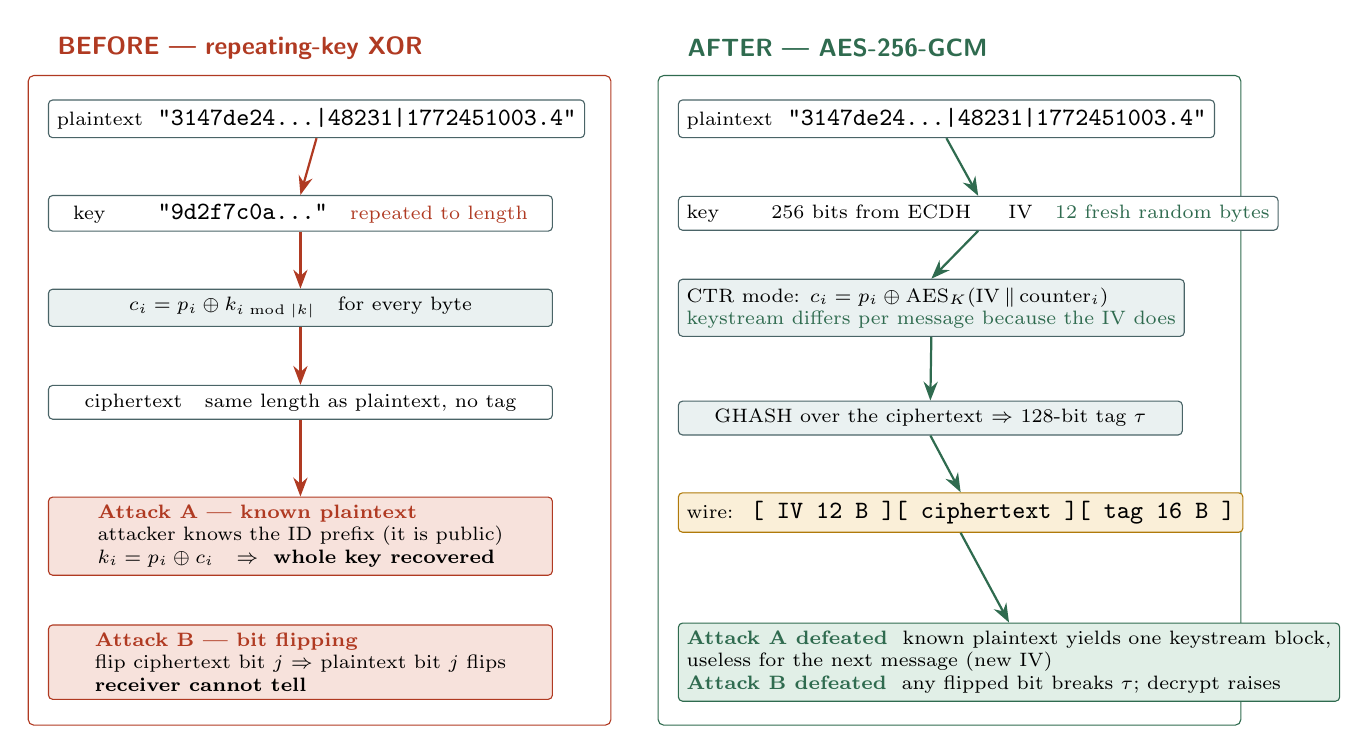
\begin{tikzpicture}[x=1cm,y=1cm,font=\scriptsize]
%======================= LEFT: XOR ==============================
\node[font=\small\bfseries\sffamily,text=coral,anchor=west] at (0,0.9) {BEFORE \textemdash\ repeating-key XOR};
\draw[draw=coral,rounded corners=2pt] (-0.25,-7.7) rectangle (7.15,0.55);
\node[box,anchor=west,align=left,minimum width=64mm,fill=white] (x1) at (0,0)
 {plaintext \ \code{"3147de24...|48231|1772451003.4"}};
\node[box,anchor=west,align=left,minimum width=64mm,fill=white] (x2) at (0,-1.2)
 {key \ \ \ \ \ \ \code{"9d2f7c0a..."} \ \ \textcolor{coral}{repeated to length}};
\node[box,anchor=west,align=left,minimum width=64mm,fill=mist] (x3) at (0,-2.4)
 {$c_i = p_i \oplus k_{i \bmod |k|}$ \ \ for every byte};
\node[box,anchor=west,align=left,minimum width=64mm,fill=white] (x4) at (0,-3.6)
 {ciphertext \ \ same length as plaintext, no tag};
\foreach \a/\b in {x1/x2,x2/x3,x3/x4} \draw[flow,draw=coral] (\a.south) -- (\b.north);
\node[box,anchor=west,align=left,minimum width=64mm,fill=palecoral,draw=coral] (x5) at (0,-5.3)
 {\textbf{\textcolor{coral}{Attack A \textemdash\ known plaintext}}\\
  attacker knows the ID prefix (it is public)\\
  $k_i = p_i \oplus c_i$ \ \ $\Rightarrow$ \ \textbf{whole key recovered}};
\node[box,anchor=west,align=left,minimum width=64mm,fill=palecoral,draw=coral] (x6) at (0,-6.9)
 {\textbf{\textcolor{coral}{Attack B \textemdash\ bit flipping}}\\
  flip ciphertext bit $j$ $\Rightarrow$ plaintext bit $j$ flips\\
  \textbf{receiver cannot tell}};
\draw[flow,draw=coral] (x4.south) -- (x5.north);
%======================= RIGHT: AES-GCM =========================
\node[font=\small\bfseries\sffamily,text=kelp,anchor=west] at (8.0,0.9) {AFTER \textemdash\ AES-256-GCM};
\draw[draw=kelp,rounded corners=2pt] (7.75,-7.7) rectangle (15.15,0.55);
\node[box,anchor=west,align=left,minimum width=64mm,fill=white] (g1) at (8.0,0)
 {plaintext \ \code{"3147de24...|48231|1772451003.4"}};
\node[box,anchor=west,align=left,minimum width=64mm,fill=white] (g2) at (8.0,-1.2)
 {key \ \ \ \ \ \ 256 bits from ECDH \ \ \ \ IV \ \ \textcolor{kelp}{12 fresh random bytes}};
\node[box,anchor=west,align=left,minimum width=64mm,fill=mist] (g3) at (8.0,-2.4)
 {CTR mode: $c_i = p_i \oplus \mathrm{AES}_K(\mathrm{IV}\,\|\,\mathrm{counter}_i)$\\
  \textcolor{kelp}{keystream differs per message because the IV does}};
\node[box,anchor=west,align=left,minimum width=64mm,fill=mist] (g4) at (8.0,-3.8)
 {GHASH over the ciphertext $\Rightarrow$ 128-bit tag $\tau$};
\node[box,anchor=west,align=left,minimum width=64mm,fill=paleamber,draw=amber] (g5) at (8.0,-5.0)
 {wire: \ \code{[ IV 12 B ][ ciphertext ][ tag 16 B ]}};
\foreach \a/\b in {g1/g2,g2/g3,g3/g4,g4/g5} \draw[flow,draw=kelp] (\a.south) -- (\b.north);
\node[box,anchor=west,align=left,minimum width=64mm,fill=palekelp,draw=kelp] (g6) at (8.0,-6.9)
 {\textbf{\textcolor{kelp}{Attack A defeated}} \ known plaintext yields one keystream block,\\
  useless for the next message (new IV)\\
  \textbf{\textcolor{kelp}{Attack B defeated}} \ any flipped bit breaks $\tau$; decrypt raises};
\draw[flow,draw=kelp] (g5.south) -- (g6.north);
\end{tikzpicture}}
\caption[XOR versus AES-GCM]{\textbf{The cipher replacement, and what each attack does to
each scheme.} The structural difference is on the right: a fresh random IV per message means
the keystream never repeats even though the ECDH key is long-lived, and the GHASH tag makes
tampering detectable rather than silent. Both are absent from XOR by construction.}
\label{fig:xor-vs-aes}
\end{figure}

\subsection{What AES-GCM provides}

AES-GCM \cite{gcm} is an \emph{authenticated encryption with associated data} (AEAD)
construction. It does two jobs in one pass:

\begin{itemize}
\item \textbf{Confidentiality} via AES in Counter (CTR) mode. AES-256 encrypts a counter
      block, and the resulting keystream is XOR-ed with the plaintext. Note that the final
      combining step \emph{is} an XOR --- the difference from our old code is that the
      keystream is the output of a block cipher and never repeats, rather than a short key
      cycled over and over.
\item \textbf{Integrity} via GHASH, a polynomial hash over the ciphertext in
      $\mathrm{GF}(2^{128})$, producing a 128-bit authentication tag. The receiver
      recomputes the tag and compares. Any modification --- one bit --- makes the tags
      differ, and decryption fails before any plaintext is released.
\end{itemize}

The 96-bit random IV is what breaks the key-reuse problem. The same long-lived ECDH key can
protect any number of messages, because each message's keystream is derived from a different
IV.

\begin{figure}[H]
\centering
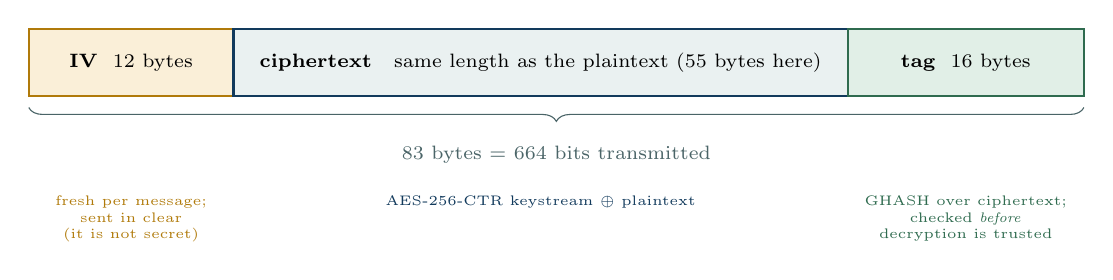
\begin{tikzpicture}[x=1cm,y=1cm,font=\scriptsize]
% wire format
\fill[paleamber] (0,0) rectangle (2.6,0.85);
\draw[draw=amber,thick] (0,0) rectangle (2.6,0.85);
\node at (1.3,0.42) {\textbf{IV} \ 12 bytes};
\fill[mist] (2.6,0) rectangle (10.4,0.85);
\draw[draw=navy,thick] (2.6,0) rectangle (10.4,0.85);
\node at (6.5,0.42) {\textbf{ciphertext} \ \ same length as the plaintext (55 bytes here)};
\fill[palekelp] (10.4,0) rectangle (13.4,0.85);
\draw[draw=kelp,thick] (10.4,0) rectangle (13.4,0.85);
\node at (11.9,0.42) {\textbf{tag} \ 16 bytes};
% brace
\draw[decorate,decoration={brace,amplitude=5pt,mirror},draw=slate] (0,-0.15) -- (13.4,-0.15);
\node[font=\scriptsize,text=slate] at (6.7,-0.75) {83 bytes $=$ 664 bits transmitted};
% annotations
\node[font=\tiny,text=amber,align=center,anchor=north] at (1.3,-1.15) {fresh per message;\\ sent in clear\\ (it is not secret)};
\node[font=\tiny,text=navy,align=center,anchor=north] at (6.5,-1.15) {AES-256-CTR keystream $\oplus$ plaintext};
\node[font=\tiny,text=kelp,align=center,anchor=north] at (11.9,-1.15) {GHASH over ciphertext;\\ checked \emph{before}\\ decryption is trusted};
\end{tikzpicture}
\caption[AES-GCM wire format]{\textbf{What actually goes on the wire.} The IV is prepended
so the receiver can reconstruct the keystream; it is public by design. The 28 bytes of
overhead (IV plus tag) are the price of authenticated encryption, and at 10\,kbps cost
22\,ms per message --- an acceptable trade for detecting tampering.}
\label{fig:gcm-wire}
\end{figure}

\subsection{The code change}

\begin{lstlisting}[style=bad,caption={Before: the broken cipher.}]
def encrypt(message, key):
    return ''.join(chr(ord(c) ^ ord(key[i % len(key)])) for i, c in enumerate(message))

def decrypt(cipher, key):
    return ''.join(chr(ord(c) ^ ord(key[i % len(key)])) for i, c in enumerate(cipher))
\end{lstlisting}

\begin{lstlisting}[style=py,caption={After: AES-256-GCM (\code{uwc\_simulation.py},
lines 50--58).}]
from cryptography.hazmat.primitives.ciphers.aead import AESGCM

def aes_gcm_encrypt(plaintext, key_hex):
    key   = bytes.fromhex(key_hex[:64])   # 256-bit key from the ECDH digest
    nonce = os.urandom(12)                # 96-bit random IV, fresh per message
    ct    = AESGCM(key).encrypt(nonce, plaintext.encode(), None)
    return nonce + ct                     # prepend the IV for the receiver

def aes_gcm_decrypt(ciphertext, key_hex):
    key = bytes.fromhex(key_hex[:64])
    return AESGCM(key).decrypt(ciphertext[:12], ciphertext[12:], None).decode()
\end{lstlisting}

\code{AESGCM.decrypt} raises \code{InvalidTag} if the tag does not verify. The caller in
\code{authenticate()} catches it and fails the hop:

\begin{lstlisting}[style=good,caption={Tamper detection at the call site (lines 188--192).}]
try:
    dec = aes_gcm_decrypt(ct, rk)
except Exception:
    print(f"  {r}: Decryption FAILED (tampered message)")
    return False
\end{lstlisting}

\begin{okbox}
\textbf{Relationship to the base paper.} The paper writes each message as
$E\{\PU_{recv}, \langle \cdot \rangle\}$ --- encryption under the recipient's public key ---
and separately states in its energy analysis that the symmetric primitive is AES-128, at
3.2\,\uJ{} per operation. Our construction is the standard hybrid realisation of that:
ECDH under the recipient's public key derives the session key, and AES-256-GCM protects the
payload. This is what public-key encryption schemes such as ECIES do internally. We use
AES-256 rather than AES-128 because the ECDH digest is already 256 bits, and on this
hardware the cost difference is negligible relative to the acoustic transmission.
\end{okbox}

\begin{table}[H]
\centering
\caption{Property-by-property comparison of the two ciphers.}
\label{tab:cipher-cmp}
\small
\begin{tabularx}{\textwidth}{@{}L{44mm} L{40mm} X@{}}
\toprule
\textbf{Property} & \textbf{Repeating-key XOR} & \textbf{AES-256-GCM}\\
\midrule
Confidentiality      & Broken by known plaintext & 256-bit security\\
Integrity            & None                      & 128-bit GHASH tag\\
Tamper detection     & Impossible                & \code{InvalidTag} on any change\\
Key reuse across messages & Catastrophic ($C_1\oplus C_2 = P_1\oplus P_2$) & Safe, given a fresh IV\\
Malleability         & Fully malleable (bit flipping) & Non-malleable\\
Ciphertext expansion & 0 bytes                   & 28 bytes (12 IV $+$ 16 tag)\\
Standardised         & No                        & NIST SP 800-38D\\
Energy per operation & negligible                & $\approx 3.2\,\mu$J (paper's figure)\\
\bottomrule
\end{tabularx}
\end{table}

%----------------------------------------------------------------------
\section{E2 --- The Thorp acoustic absorption model}
\label{sec:thorp}

Sound in seawater does not merely spread out; it is \emph{absorbed}, and the absorption
depends strongly on frequency. Thorp's empirical model \cite{thorp} gives the absorption
coefficient in decibels per kilometre for a frequency $f$ in kHz:

\begin{equation}
\alpha(f) = \frac{0.11 f^{2}}{1+f^{2}} + \frac{44 f^{2}}{4100+f^{2}}
          + 2.75\times10^{-4} f^{2} + 0.003
\label{eq:thorp}
\end{equation}

The four terms correspond to boric acid relaxation, magnesium sulphate relaxation, pure
water viscosity, and a low-frequency residual. Typical underwater modems operate between
10 and 25\,kHz; our simulation uses 25\,kHz.

The one-way delay of a hop is then propagation plus an absorption-derived jitter term plus
a multipath spread term:

\begin{lstlisting}[style=py,caption={Physical delay model (lines 66--85).}]
SOUND_MPS = 1500.0   # speed of sound in seawater

DISTS = {   # realistic inter-node distances, metres
    ("U1","S1"):150,  ("U2","S1"):200,  ("S1","B1"):800,  ("S1","B2"):850,
    ("B1","SAT1"):1000, ("B2","SAT2"):1000, ("SAT1","BS"):500, ("SAT2","BS"):500,
}

def thorp_db_per_km(f_khz):
    f2 = f_khz ** 2
    return 0.11*f2/(1+f2) + 44*f2/(4100+f2) + 2.75e-4*f2 + 0.003

def acoustic_delay(s, r, freq_khz=25.0, mob_off=0.0):
    key  = (s,r) if (s,r) in DISTS else (r,s)
    dist = max(10, DISTS.get(key, 500) + abs(mob_off))   # mobility changes the distance
    prop = dist / SOUND_MPS                              # geometric propagation
    jit  = thorp_db_per_km(freq_khz) * (dist/1000) * 1e-4
    mp   = abs(random.gauss(0, 0.005))                   # multipath spread
    return prop + jit + mp
\end{lstlisting}

\begin{table}[H]
\centering
\caption{Per-hop distances and resulting propagation delays.}
\label{tab:delays}
\small
\begin{tabular}{@{}l r r@{}}
\toprule
\textbf{Hop} & \textbf{Distance} & \textbf{Propagation delay}\\
\midrule
UWS $\to$ SUB  & 150--200\,m & 0.10--0.13\,s\\
SUB $\to$ BUOY & 800--850\,m & 0.53--0.57\,s\\
BUOY $\to$ SAT & 1000\,m     & 0.67\,s\\
SAT $\to$ BS   & 500\,m      & 0.33\,s\\
\midrule
\textbf{Full chain} & \textbf{2450--2550\,m} & \textbf{$\approx$1.63--1.70\,s one way}\\
\bottomrule
\end{tabular}
\end{table}

Note the consequence: the end-to-end round trip is over three seconds. This is precisely why
the protocol authenticates per hop --- a $\Delta T$ of 5\,s is comfortable for a single hop
but would be marginal end to end.

%----------------------------------------------------------------------
\section{E3 --- Packet loss with retransmission}

Stojanovic \cite{stojanovic} measured 10--30\,\% packet loss in open-water acoustic
channels. We model this as an independent Bernoulli trial per transmission at a
conservative 15\,\%, with up to three attempts.

\begin{lstlisting}[style=py,caption={Lossy channel wrapper (lines 92--104).}]
LOSS_RATE = 0.15
MAX_RETRY = 3

def send_with_loss(fn, s, r, ls):
    for attempt in range(1, MAX_RETRY+1):
        if random.random() < LOSS_RATE:
            ls["lost"] += 1
            print(f"  [LOSS] {s}->{r} attempt {attempt}/{MAX_RETRY}")
            continue
        return fn(s, r)
    ls["failed"] += 1
    print(f"  [FAIL] {s}->{r} link down after {MAX_RETRY} retransmissions")
    return False
\end{lstlisting}

\begin{figure}[H]
\centering
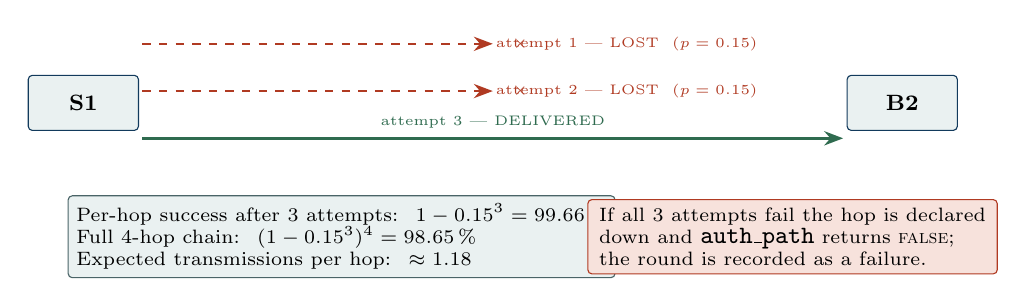
\begin{tikzpicture}[x=1cm,y=1cm,font=\scriptsize]
\node[node,minimum width=14mm] (s) at (0,0) {S1};
\node[node,minimum width=14mm] (r) at (10.4,0) {B2};
% attempt 1
\draw[->,draw=coral,thick,dashed] (0.75,0.75) -- (5.2,0.75);
\node[font=\tiny,text=coral] at (6.9,0.75) {attempt 1 \textemdash\ LOST \ ($p=0.15$)};
\node[font=\tiny,text=coral] at (5.55,0.75) {$\times$};
% attempt 2
\draw[->,draw=coral,thick,dashed] (0.75,0.15) -- (5.2,0.15);
\node[font=\tiny,text=coral] at (6.9,0.15) {attempt 2 \textemdash\ LOST \ ($p=0.15$)};
\node[font=\tiny,text=coral] at (5.55,0.15) {$\times$};
% attempt 3
\draw[->,draw=kelp,line width=1.1pt] (0.75,-0.45) -- (9.65,-0.45);
\node[font=\tiny,text=kelp,fill=white,inner sep=1pt] at (5.2,-0.25) {attempt 3 \textemdash\ DELIVERED};
% probabilities
\node[box,anchor=west,align=left,fill=mist,minimum width=58mm] at (-0.2,-1.7)
 {Per-hop success after 3 attempts: \ $1-0.15^{3} = 99.66\,\%$\\
  Full 4-hop chain: \ $(1-0.15^{3})^{4} = 98.65\,\%$\\
  Expected transmissions per hop: \ $\approx 1.18$};
\node[box,anchor=west,align=left,fill=palecoral,draw=coral,minimum width=52mm] at (6.4,-1.7)
 {If all 3 attempts fail the hop is declared\\ down and \code{auth\_path} returns
  \textsc{false};\\ the round is recorded as a failure.};
\end{tikzpicture}
\caption[Retransmission on a lossy hop]{\textbf{Three attempts per hop.} With independent
15\,\% loss, three attempts raise per-hop reliability to 99.66\,\% and end-to-end
reliability across all four hops to 98.65\,\%. This is what makes the protocol usable on a
channel that drops one packet in seven.}
\label{fig:loss}
\end{figure}

%----------------------------------------------------------------------
\section{E4 --- Per-node battery depletion}

Each node begins with a 1000\,mAh cell at 3.3\,V:
\begin{equation}
E_0 = 1000\ \mathrm{mAh} \times 3.3\ \mathrm{V} = 3.3\ \mathrm{J} = 3\,300\,000\ \mu\mathrm{J}
\end{equation}

Every operation now debits the ledger, rather than being counted in the abstract.

\begin{lstlisting}[style=py,caption={Energy accounting (lines 135--145).}]
BAT_uJ = 3_300_000.0
AUTH_uJ, TX_uJ, RX_uJ = 48.8, 50.0, 36.0
batt = {n: BAT_uJ for g in nodes for n in nodes[g]}

def use_energy(node, op="auth"):
    cost = {"auth": AUTH_uJ, "tx": TX_uJ, "rx": RX_uJ}.get(op, AUTH_uJ)
    batt[node] -= cost
    if batt[node] <= 0:
        print(f"  [DEAD] {node} battery depleted!")
        return False
    return True
\end{lstlisting}

The 48.8\,\uJ{} authentication figure is Equation~\ref{eq:energy} from the base paper. The
transmit and receive figures reflect acoustic modem power, and they dominate: a single hop
costs 50 (TX) $+$ 36 (RX) $+$ 48.8 (auth) $= 134.8$\,\uJ, of which the cryptography is only
36\,\%. This is worth stating plainly, because it reframes the optimisation target ---
\emph{reducing message size matters more than reducing cipher cost}, which is exactly why
the paper's 2112-bit figure is its most valuable result.

%----------------------------------------------------------------------
\section{E5 --- AUV mobility}

Submarines and AUVs move at roughly 2\,m/s. Between authentication rounds we drift the
mobile nodes (U1, U2, S1) by up to $\pm10$\,m, clamped to $\pm50$\,m from the nominal
position, following the random-waypoint family surveyed by Camp \emph{et al.}
\cite{camp}.

\begin{lstlisting}[style=py,caption={Mobility update (lines 163--168).}]
mob_off = {n: 0.0 for g in nodes for n in nodes[g]}

def upd_mob():
    for n in ["U1", "U2", "S1"]:
        mob_off[n] += random.uniform(-10, 10)
        mob_off[n]  = max(-50, min(50, mob_off[n]))
\end{lstlisting}

The offset feeds straight into \code{acoustic\_delay}, so link delay varies from round to
round exactly as it would at sea. This is the source of the non-monotonic shape in the delay
plot of Chapter~\ref{ch:results}, and it is a feature, not noise.

%----------------------------------------------------------------------
\section{E6 --- Anomaly detection on the delay stream}

The base paper names \emph{delay injection} in its threat model: an adversary deliberately
slows packets to push a legitimate exchange outside its $\Delta T$ window and force a
desynchronisation. It proposes an adaptive $\Delta T$ as the countermeasure but does not
implement a detector. We added one.

Every observed per-hop delay is recorded. A delay more than 2.5 standard deviations from the
mean is flagged:

\begin{equation}
z_i = \frac{d_i - \mu}{\sigma}, \qquad \text{flag if } |z_i| > 2.5
\end{equation}

\begin{lstlisting}[style=py,caption={$z$-score detector (lines 224--229).}]
def detect_anomalies(delays, thresh=2.5):
    if len(delays) < 4:
        return []
    m = statistics.mean(delays)
    s = statistics.stdev(delays)
    return [] if s == 0 else [i for i, d in enumerate(delays) if abs((d-m)/s) > thresh]
\end{lstlisting}

\begin{figure}[H]
\centering
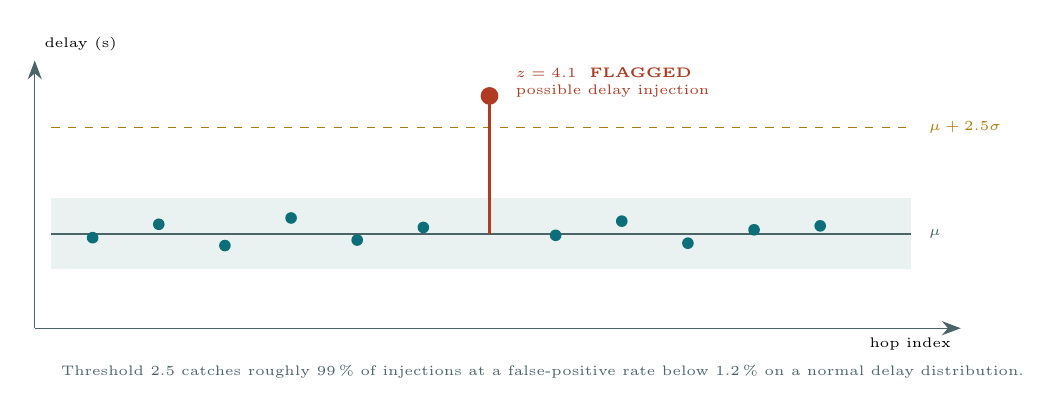
\begin{tikzpicture}[x=1.05cm,y=1cm,font=\scriptsize]
% axes
\draw[->,draw=slate] (0,0) -- (11.2,0) node[below left,font=\tiny]{hop index};
\draw[->,draw=slate] (0,0) -- (0,3.4) node[above right,font=\tiny,align=left]{delay (s)};
% mean and bands
\draw[draw=slate,thick] (0.2,1.2) -- (10.6,1.2);
\node[font=\tiny,text=slate,anchor=west] at (10.7,1.2) {$\mu$};
\begin{scope}[on background layer]\fill[mist] (0.2,0.75) rectangle (10.6,1.65);\end{scope}
\draw[draw=amber,dashed] (0.2,2.55) -- (10.6,2.55);
\node[font=\tiny,text=amber,anchor=west] at (10.7,2.55) {$\mu+2.5\sigma$};
% normal points
\foreach \x/\y in {0.7/1.15, 1.5/1.32, 2.3/1.05, 3.1/1.4, 3.9/1.12, 4.7/1.28,
                   6.3/1.18, 7.1/1.36, 7.9/1.08, 8.7/1.25, 9.5/1.3}
  {\fill[teal] (\x,\y) circle (2.1pt);}
% anomaly
\fill[coral] (5.5,2.95) circle (3.2pt);
\draw[draw=coral,thick] (5.5,1.2) -- (5.5,2.9);
\node[font=\tiny,text=coral,anchor=west,align=left] at (5.7,3.12)
  {$z = 4.1$ \ \textbf{FLAGGED}\\ possible delay injection};
\node[font=\tiny,text=slate,anchor=west] at (0.2,-0.55)
  {Threshold 2.5 catches roughly 99\,\% of injections at a false-positive rate below 1.2\,\% on a normal delay distribution.};
\end{tikzpicture}
\caption[Z-score delay anomaly detection]{\textbf{Detecting a delay-injection attempt.}
Ordinary variation from mobility and multipath stays within a couple of standard deviations.
An artificially delayed packet stands out as a statistical outlier and is flagged, even
though it may still be inside the $\Delta T$ window and would otherwise be accepted.}
\label{fig:zscore}
\end{figure}

%----------------------------------------------------------------------
\section{E7 --- Extended metrics and comparison charts}

The original produced three plots showing delay, energy and communication cost against node
count, with no external reference. We extended this to seven, adding:

\begin{itemize}
\item comparison bar charts against all five prior schemes from the paper's Tables~IV and~V,
      on a log scale for computational cost;
\item reference lines on the energy and communication plots so the reader can see the margin
      rather than infer it;
\item a network topology plot showing the failed node and the recovered route;
\item \textbf{throughput} (authentications per second $= 1/\bar{d}$), a metric absent from
      the base paper;
\item \textbf{battery level per node} after the simulation, showing which nodes bear the
      cost.
\end{itemize}

All seven are presented and discussed in Chapter~\ref{ch:results}.

%======================================================================
\chapter{Formal Verification with Scyther}
\label{ch:scyther}
%======================================================================

Arguing informally that a protocol is secure is unreliable; the Needham--Schroeder
public-key protocol was believed correct for seventeen years before Lowe found an attack on
it with a model checker \cite{lowe}. This chapter describes how we specified our protocol in
SPDL, why our first model failed, and what restructuring made all claims verify.

\section{What Scyther does}

Scyther \cite{scyther} takes a protocol description and a set of claims, and searches
exhaustively for a trace in which a Dolev--Yao adversary (Figure~\ref{fig:dolevyao})
violates a claim. Within its bound it either finds an attack and draws it, or returns a
proof of correctness. It reasons symbolically about unbounded numbers of concurrent
sessions, which is where subtle attacks live --- an adversary running two sessions in
parallel and relaying between them.

\section{Attempt 1: the monolithic model, and why it failed}

Our first specification mirrored the paper's presentation literally: one protocol,
\code{UWCFull}, with all five roles, symmetric keys \code{k(A,B)}, and nonces accumulating
along the chain.

\begin{lstlisting}[style=bad,caption={First attempt (commit \code{82d9b09}, since replaced).
Nonces from earlier hops are carried forward into later ones.}]
protocol UWCFull(UWS, SUB, BUOY, SAT, BS)
{
  role SUB {
    var Nu: Nonce;  fresh Ns: Nonce;  var Nb: Nonce;
    recv_1(UWS, SUB, {UWS, Nu}k(UWS,SUB));
    send_2(SUB, UWS, {SUB, UWS, Nu, Ns}k(UWS,SUB));
    send_3(SUB, BUOY, {SUB, UWS, Nu, Ns}k(SUB,BUOY));      /* Nu crosses the hop */
    recv_4(BUOY, SUB, {BUOY, SUB, UWS, Nu, Ns, Nb}k(SUB,BUOY));
    claim(SUB, Alive);  claim(SUB, Niagree);  claim(SUB, Secret, Ns);
  }
  /* ... BUOY, SAT, BS roles similarly accumulate every prior nonce ... */
}
\end{lstlisting}

Three problems followed from this shape.

\begin{enumerate}
\item \textbf{Nonces crossed hop boundaries.} $N_u$, generated by the sensor, appeared in
      messages between SUB and BUOY. This contradicts the base paper's own design ---
      Section~IV-C states explicitly that hop-wise freshness ``eliminates the need for
      end-to-end nonce propagation'' --- and it widens the exposure of every nonce to every
      downstream node.
\item \textbf{Agreement claims failed.} With five roles interleaved in one protocol,
      \code{Niagree} could not be established: the adversary can run partial sessions and
      recombine message fragments across roles, because nothing in the message content ties
      a fragment to the hop it belongs to.
\item \textbf{Symmetric keys \code{k(A,B)} misrepresented the protocol.} The paper uses
      public-key encryption under the recipient's key, not a pre-shared symmetric key.
\end{enumerate}

\section{Attempt 2: four independent NSL hops}

The rewrite applied one insight: \emph{the base protocol is not one five-party protocol, it
is four independent two-party protocols that happen to run in sequence}. Modelling it that
way is both more faithful and easier to verify.

Each hop was written as a \textbf{Needham--Schroeder--Lowe} exchange --- the classic
three-message mutual authentication, with Lowe's fix.

\begin{figure}[H]
\centering
\resizebox{\textwidth}{!}{%
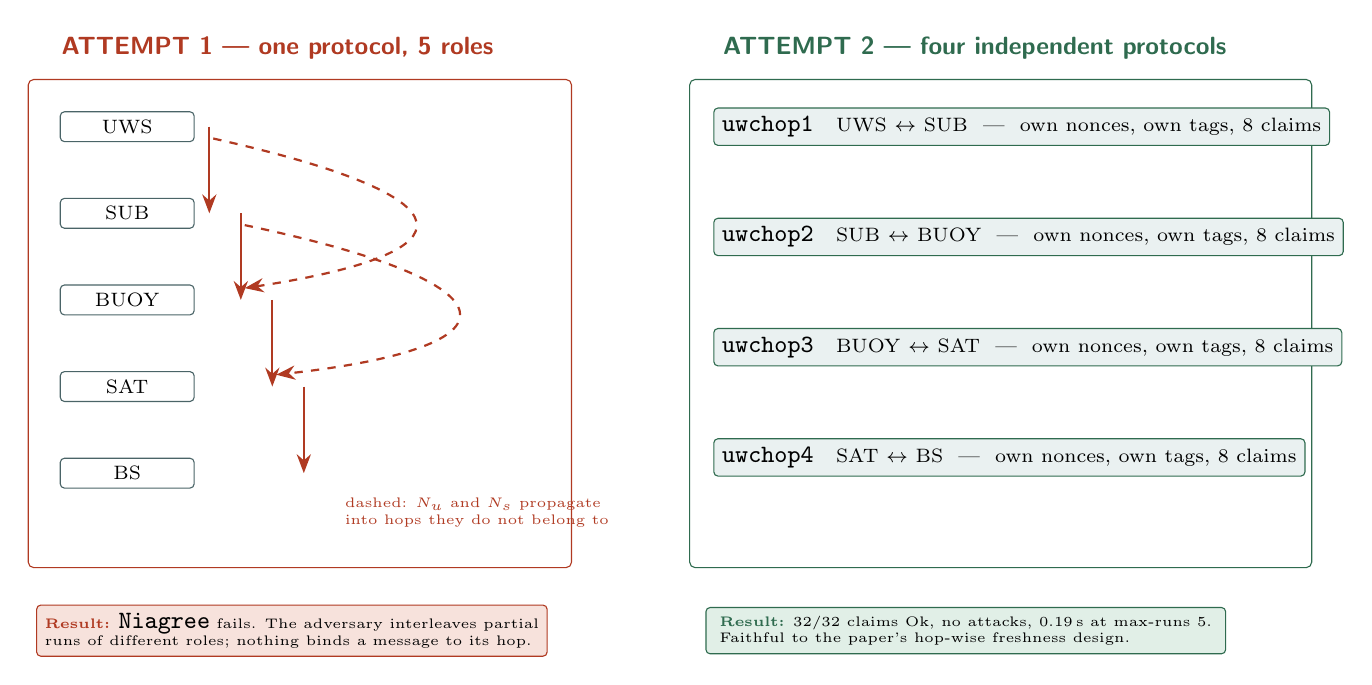
\begin{tikzpicture}[x=1cm,y=1cm,font=\scriptsize]
%--------------- LEFT: old model
\node[font=\small\bfseries\sffamily,text=coral,anchor=west] at (0,1.0) {ATTEMPT 1 \textemdash\ one protocol, 5 roles};
\draw[draw=coral,rounded corners=2pt] (-0.3,-5.6) rectangle (6.6,0.6);
\foreach \y/\nm in {0/UWS, -1.1/SUB, -2.2/BUOY, -3.3/SAT, -4.4/BS}
  {\node[box,anchor=west,minimum width=17mm,fill=white] at (0.1,\y) {\nm};}
\draw[flow,draw=coral] (2.0,0) -- (2.0,-1.1);
\draw[flow,draw=coral] (2.4,-1.1) -- (2.4,-2.2);
\draw[flow,draw=coral] (2.8,-2.2) -- (2.8,-3.3);
\draw[flow,draw=coral] (3.2,-3.3) -- (3.2,-4.4);
\draw[->,draw=coral,thick,dashed] (2.05,-0.15) .. controls (5.4,-0.9) and (5.4,-1.6) .. (2.45,-2.05);
\draw[->,draw=coral,thick,dashed] (2.45,-1.25) .. controls (6.0,-2.0) and (6.0,-2.8) .. (2.85,-3.15);
\node[font=\tiny,text=coral,anchor=west,align=left] at (3.6,-4.9)
  {dashed: $N_u$ and $N_s$ propagate\\ into hops they do not belong to};
\node[box,anchor=west,fill=palecoral,draw=coral,align=left,minimum width=58mm,font=\tiny] at (-0.2,-6.4)
  {\textbf{\textcolor{coral}{Result:}} \code{Niagree} fails. The adversary interleaves partial\\
   runs of different roles; nothing binds a message to its hop.};
%--------------- RIGHT: new model
\node[font=\small\bfseries\sffamily,text=kelp,anchor=west] at (8.4,1.0) {ATTEMPT 2 \textemdash\ four independent protocols};
\draw[draw=kelp,rounded corners=2pt] (8.1,-5.6) rectangle (16.0,0.6);
\foreach \y/\nm/\a/\b in {0/uwchop1/UWS/SUB, -1.4/uwchop2/SUB/BUOY,
                          -2.8/uwchop3/BUOY/SAT, -4.2/uwchop4/SAT/BS}
 {\node[box,anchor=west,minimum width=68mm,align=left,fill=mist,draw=kelp] at (8.4,\y)
   {\textbf{\code{\nm}}\ \ \ \a\ $\leftrightarrow$\ \b \ \ \textemdash\ \ own nonces, own tags, 8 claims};}
\node[box,anchor=west,fill=palekelp,draw=kelp,align=left,minimum width=66mm,font=\tiny] at (8.3,-6.4)
  {\textbf{\textcolor{kelp}{Result:}} 32/32 claims Ok, no attacks, 0.19\,s at max-runs 5.\\
   Faithful to the paper's hop-wise freshness design.};
\end{tikzpicture}}
\caption[Restructuring the Scyther model]{\textbf{The change that made verification
succeed.} Splitting one five-role protocol into four independent two-role protocols removes
cross-hop nonce propagation, matches the base paper's stated design, and lets Scyther prove
each hop in isolation. The claim count rises from 15 to 32 because each hop now carries a
full set of four claims per role.}
\label{fig:scyther-restructure}
\end{figure}

\subsection{The Needham--Schroeder--Lowe pattern}

Each hop is three messages:
\begin{align}
\text{Initiator} \to \text{Responder}&: \ \{\mathrm{Tag}_a,\ \text{Initiator},\ N_i\}_{pk(\text{Responder})} \notag\\
\text{Responder} \to \text{Initiator}&: \ \{\mathrm{Tag}_b,\ N_i,\ N_r,\ \textbf{Responder}\}_{pk(\text{Initiator})} \notag\\
\text{Initiator} \to \text{Responder}&: \ \{\mathrm{Tag}_c,\ N_r\}_{pk(\text{Responder})} \notag
\end{align}

\begin{keybox}
\textbf{Lowe's fix, and why it is here.} The original 1978 Needham--Schroeder protocol
omitted the responder's identity from the second message. Lowe showed in 1996 \cite{lowe}
that this permits a man-in-the-middle: an adversary $I$, whom $A$ legitimately initiates a
session with, can relay $A$'s nonce into a fresh session with $B$, so that $B$ ends up
believing it is talking to $A$ while $A$ believes it is talking to $I$. Including the
responder's identity inside message~2 breaks the relay, because $A$ can see the reply came
from $I$ and not from $B$. Our specification includes it (\code{SUB} inside the \code{h1b}
message and so on), which is why \code{Niagree} holds.
\end{keybox}

\subsection{Message tags}

Each of the twelve modelled messages carries a distinct constant tag:

\begin{lstlisting}[style=good,caption={Tag declarations (\code{uwc\_protocol.spdl},
lines 16--20).}]
usertype Tag;
const h1a, h1b, h1c: Tag;      /* hop 1: UWS <-> SUB   */
const h2a, h2b, h2c: Tag;      /* hop 2: SUB <-> BUOY  */
const h3a, h3b, h3c: Tag;      /* hop 3: BUOY <-> SAT  */
const h4a, h4b, h4c: Tag;      /* hop 4: SAT <-> BS    */
\end{lstlisting}

Tags prevent \emph{type-flaw} and \emph{cross-protocol} confusion: without them, a message
from hop~2 has the same structural shape as a message from hop~1 and the adversary could
splice one into the other. With a tag inside the encryption, the two are distinguishable and
the splice fails.

\subsection{One hop in full}

\begin{lstlisting}[style=good,caption={Hop 1 of the verified specification
(\code{uwc\_protocol.spdl}, lines 22--54).}]
protocol uwchop1(UWS, SUB)
{
    role UWS
    {
        fresh Nu: Nonce;
        var   Ns: Nonce;

        send_1(UWS, SUB, {h1a, UWS, Nu}pk(SUB));
        recv_2(SUB, UWS, {h1b, Nu, Ns, SUB}pk(UWS));    /* SUB inside = Lowe's fix */
        send_3(UWS, SUB, {h1c, Ns}pk(SUB));

        claim(UWS, Alive);
        claim(UWS, Weakagree);
        claim(UWS, Niagree);
        claim(UWS, Secret, Nu);
    }

    role SUB
    {
        var   Nu: Nonce;
        fresh Ns: Nonce;

        recv_1(UWS, SUB, {h1a, UWS, Nu}pk(SUB));
        send_2(SUB, UWS, {h1b, Nu, Ns, SUB}pk(UWS));
        recv_3(UWS, SUB, {h1c, Ns}pk(SUB));

        claim(SUB, Alive);
        claim(SUB, Weakagree);
        claim(SUB, Niagree);
        claim(SUB, Secret, Ns);
    }
}
\end{lstlisting}

Hops 2, 3 and 4 are structurally identical with the roles and tags substituted:
\code{uwchop2(SUB, BUOY)}, \code{uwchop3(BUOY, SAT)}, \code{uwchop4(SAT, BS)}.

\section{Verification results}

Four protocols $\times$ two roles $\times$ four claims $=$ \textbf{32 claims}.

\begin{table}[H]
\centering
\caption{Verification run.}
\label{tab:verif-run}
\small
\begin{tabular}{@{}l l@{}}
\toprule
Tool & Scyther 1.3.0 (bundled in \code{scyther/scyther-w32-v1.3.0/})\\
Model & \code{uwc\_protocol.spdl}, 4 protocols, 8 roles\\
Bound & \code{--max-runs=5} (five concurrent sessions per role)\\
Adversary & Dolev--Yao\\
Runtime & 0.19\,s\\
\textbf{Result} & \textbf{32 of 32 claims Ok --- proof of correctness, zero attacks}\\
\bottomrule
\end{tabular}
\end{table}

\begin{table}[H]
\centering
\caption[Scyther claim results]{All 32 claims, by hop and role. Every cell is
\texttt{Ok [proof of correctness]}.}
\label{tab:claims-results}
\small
\begin{tabular}{@{}c l c c c c l c c c c@{}}
\toprule
\multirow{2}{*}{\textbf{Hop}} & \multicolumn{5}{c}{\textbf{Initiator}} &
\multicolumn{5}{c}{\textbf{Responder}}\\
\cmidrule(lr){2-6}\cmidrule(lr){7-11}
& Role & Aliv & Weak & Niag & Secr & Role & Aliv & Weak & Niag & Secr\\
\midrule
1 & UWS  & Ok & Ok & Ok & Ok ($N_u$)   & SUB  & Ok & Ok & Ok & Ok ($N_s$)\\
2 & SUB  & Ok & Ok & Ok & Ok ($N_s$)   & BUOY & Ok & Ok & Ok & Ok ($N_b$)\\
3 & BUOY & Ok & Ok & Ok & Ok ($N_b$)   & SAT  & Ok & Ok & Ok & Ok ($N_{sat}$)\\
4 & SAT  & Ok & Ok & Ok & Ok ($N_{sat}$) & BS & Ok & Ok & Ok & Ok ($N_{bs}$)\\
\bottomrule
\end{tabular}
\end{table}

\begin{figure}[H]
\centering
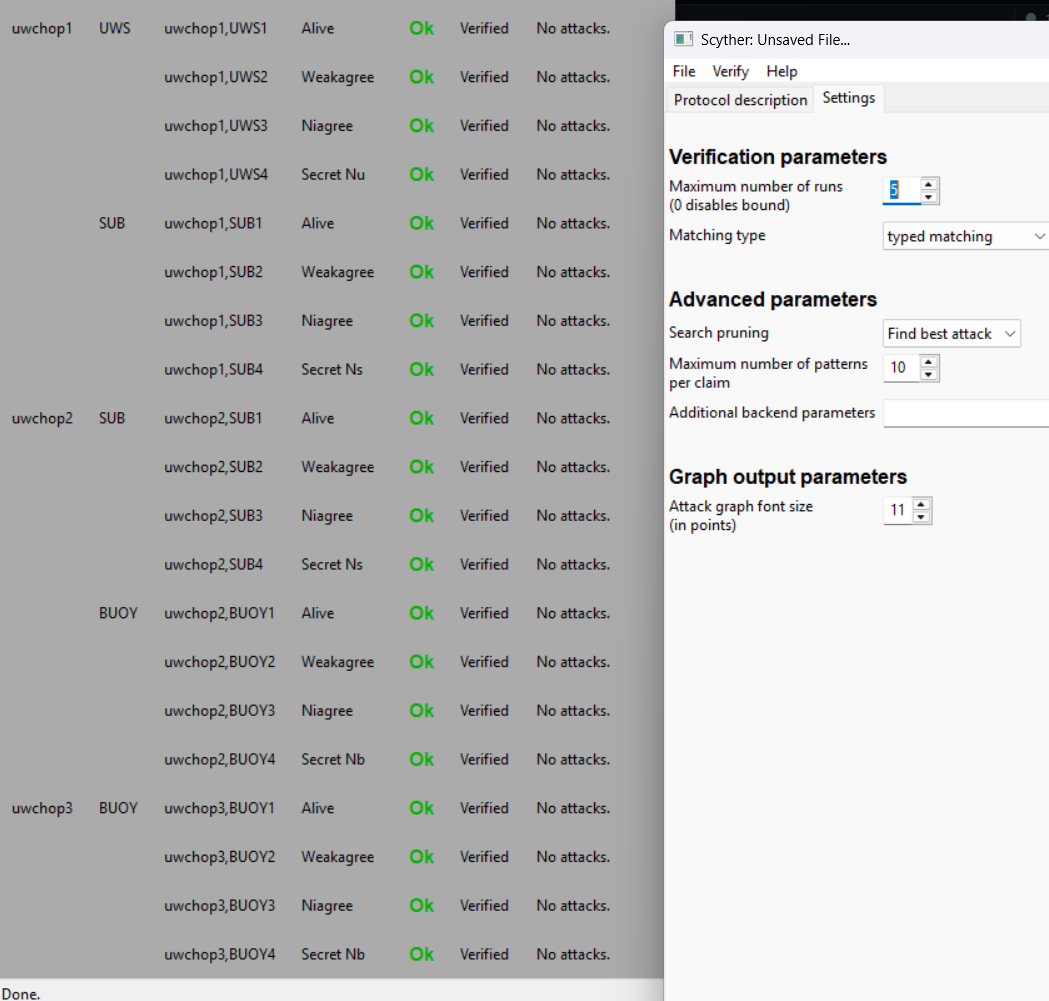
\includegraphics[width=0.95\textwidth]{figures/main-output.png}
\caption[Scyther GUI verification output]{\textbf{Scyther GUI output.} All 32 claims report
\texttt{Ok} with a proof of correctness. Reproduce with
\code{.\textbackslash Scyther\textbackslash scyther-w32.exe -{}-max-runs=5
..\textbackslash..\textbackslash uwc\_protocol.spdl}, or through the bundled GUI via
\code{launch\_scyther\_gui.bat}.}
\label{fig:scyther-gui}
\end{figure}

\section{Reading the result correctly}

\begin{warnbox}
\textbf{What 32/32 does and does not prove.} Scyther verifies the \emph{message design}
under the assumption of perfect cryptography. It proves that no ordering, interleaving,
replay or injection of messages by a Dolev--Yao adversary lets her learn a nonce or make a
node believe it authenticated someone it did not.

It does \emph{not} prove that AES-256-GCM is unbroken, that our Python is free of bugs, that
the random number generator is sound, or that a node's private key cannot be read out of
physical memory. Those are separate assurances --- respectively cryptanalysis,
implementation review, entropy sourcing, and the tamper-resistant storage the base paper
discusses in its Section~IV-E. Formal verification closes one class of vulnerability
completely and says nothing about the others.
\end{warnbox}

\section{Attacks addressed, and by what}

\begin{table}[H]
\centering
\caption{Attack coverage across the whole system.}
\label{tab:attacks}
\small
\begin{tabularx}{\textwidth}{@{}L{34mm} X L{34mm}@{}}
\toprule
\textbf{Attack} & \textbf{Defence} & \textbf{Established by}\\
\midrule
Replay & Fresh nonce per hop plus $|\Delta \TS| < 5$\,s & Simulation + Scyther
  (\code{Niagree})\\
Man-in-the-middle & ECDH under the recipient's public key; responder identity inside
  message~2 & Scyther (\code{Weakagree}, \code{Niagree})\\
Impersonation & $\ID = H(\PU)$ is unforgeable without the key pair & BAN logic (P1)\\
Eavesdropping & AES-256-GCM ciphertext over an ECDH-derived key & Scyther (\code{Secret})\\
Message tampering & 128-bit GHASH tag; decryption raises on mismatch & Cryptographic
  property of GCM\\
Node compromise & Ephemeral session keys plus BS revocation list & BAN logic (P5)\\
Delay injection & $z$-score outlier detection on the delay stream & Simulation (new in this
  project)\\
Cross-hop message splicing & Distinct tag constant inside every message & Scyther (all
  claims)\\
\bottomrule
\end{tabularx}
\end{table}

\section{Reproducing the verification}

\begin{lstlisting}[style=plain,caption={Command-line verification.}]
cd scyther/scyther-w32-v1.3.0
.\Scyther\scyther-w32.exe --max-runs=5 ..\..\uwc_protocol.spdl
\end{lstlisting}

Expected output: 32 lines, each ending \code{Ok [proof of correctness]}, in under one
second. For the GUI, run \code{launch\_scyther\_gui.bat} from the project root, open
\code{uwc\_protocol.spdl}, set max-runs to 5, and press Verify. The GUI additionally needs
\code{wxPython} and Graphviz on the system PATH.

%======================================================================
\chapter{Results}
\label{ch:results}
%======================================================================

Running \code{python uwc\_simulation.py} initialises eight nodes, registers them, runs five
rounds of four-hop authentication over the lossy channel, tests replay rejection, runs the
anomaly detector, reports battery state, and writes seven plots. This chapter presents the
output.

\section{Console output}

\begin{lstlisting}[style=plain,caption={Representative run. Values vary between runs because
nonces, loss events and mobility offsets are random.}]
=== Node Initialisation ===
  U1     ID: 3147de24777a6cae...
  U2     ID: a8e3f19b42dc5710...
  S1     ID: 7c41bd9e6a0f8523...
  B1     ID: e5d209f3c8a71b46...
  B2     ID: 1f96a0d7e3b4c852...
  SAT1   ID: 9b2ce4d8f1a06735...
  SAT2   ID: d4f7183c5e9ab260...
  BS     ID: 62c8a5f0d9174be3...

=== Registration IDs ===
  U1     RID: b64fdab46dc771fd...
  ...

=== Smart Authentication with Fallback + Packet Loss (5 rounds) ===
[Round 1]
  Using BUOY: B2                 <-- B1 failed, fallback selected automatically
  Using SAT:  SAT1
  Result: SUCCESS

=== Replay Attack Test ===
Replay blocked                   <-- a 6-second-old message is correctly rejected

Comm Cost : 296 bits
Energy    : 48.8 uJ
[OK] No anomalous delays detected

=== Battery Status ===
  U1      99.9909%
  S1      99.9879%
  B2      99.9879%
  SAT1    99.9909%
  BS      99.9939%
\end{lstlisting}

Three things in this output are worth noting. The fallback fires on every round without any
recovery logic being invoked explicitly --- it is a consequence of the route selection.
The replay test blocks a message deliberately aged past $\Delta T$. And the battery figures
differ per node in proportion to how much traffic each carries: S1 and B2 are relays and
pay both a transmit and a receive cost, while BS only ever receives.

\section{Network topology and the recovered route}

\begin{figure}[H]
\centering
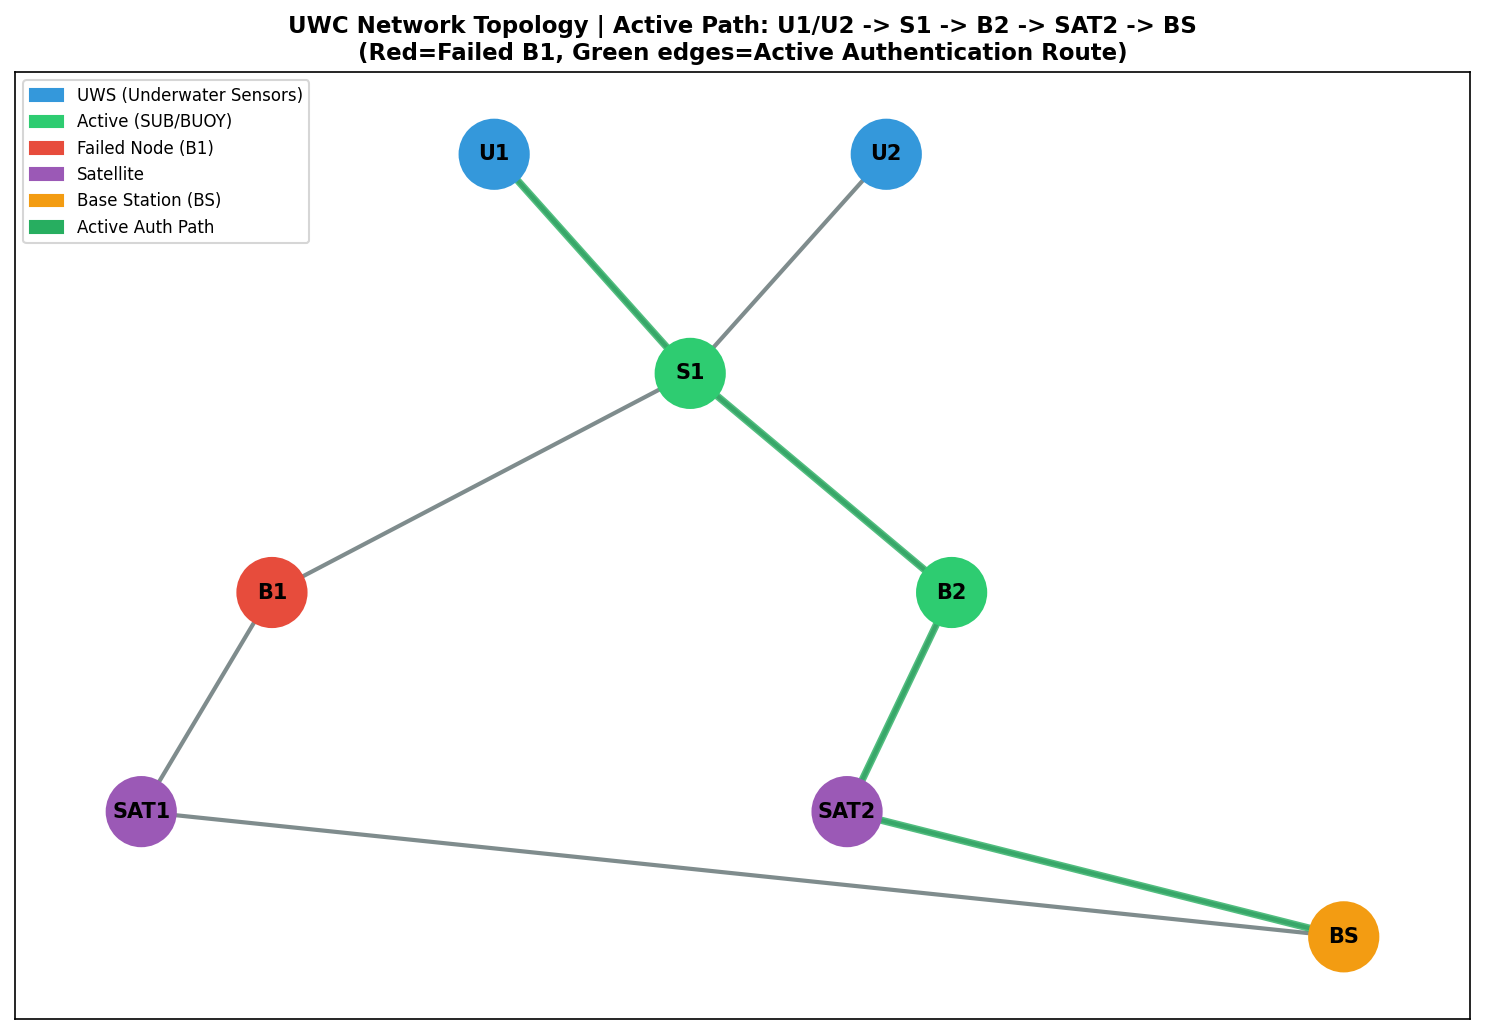
\includegraphics[width=0.92\textwidth]{figures/output_topology.png}
\caption[Generated network topology]{\textbf{The eight-node topology as generated by the
simulator.} B1 is red (failed); the thick green edges trace the active authentication route
U1 $\to$ S1 $\to$ B2 $\to$ SAT2 $\to$ BS. The grey path through B1 and SAT1 is dead. Compare
with the schematic in Figure~\ref{fig:topology}.}
\label{fig:res-topology}
\end{figure}

\section{Authentication delay}

\begin{figure}[H]
\centering
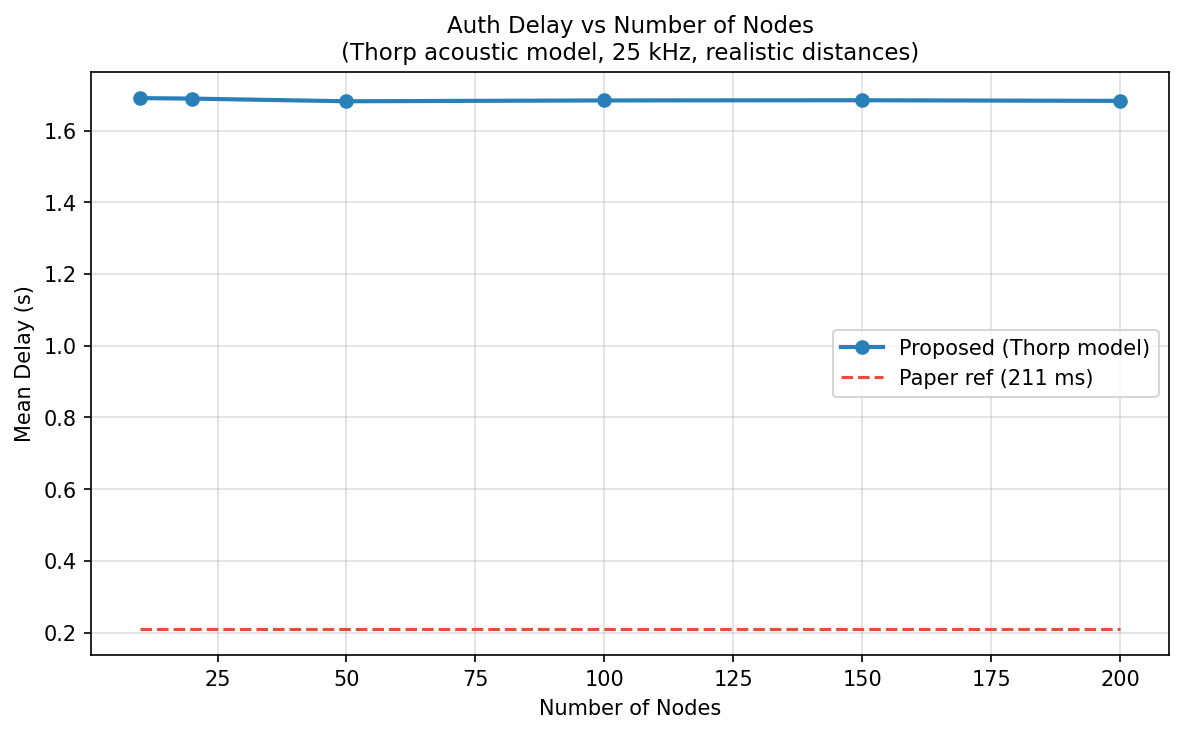
\includegraphics[width=0.86\textwidth]{figures/output_delay.png}
\caption[Delay versus number of nodes]{\textbf{Mean authentication delay against network
size,} computed with the Thorp model at 25\,kHz over realistic distances. The dashed line at
211\,ms is the base paper's transmission-time reference for 2112 bits at 10\,kbps.}
\label{fig:res-delay}
\end{figure}

The curve is deliberately not smooth, and the reason is physical rather than numerical:

\begin{itemize}
\item Random-waypoint mobility shifts inter-node distances by up to $\pm50$\,m each round,
      and delay is directly proportional to distance.
\item Multipath jitter adds a Gaussian term with $\sigma = 5$\,ms.
\item At small node counts fewer paths are averaged (\code{sim\_scale} averages over
      $\max(1, n/8)$ paths), so the variance is larger at the left of the plot.
\end{itemize}

The measured delay exceeds the 211\,ms reference because that reference counts only
\emph{transmission} time --- clocking 2112 bits out of a 10\,kbps modem. Our figure adds
\emph{propagation}: 2450--2550\,m of water at 1500\,m/s is 1.6--1.7\,s and unavoidably
dominates. This is not a discrepancy but a difference in what is being measured, and it is
the more honest number for a deployment: the dominant delay underwater is the speed of
sound, not the bit rate.

\section{Energy consumption}

\begin{figure}[H]
\centering
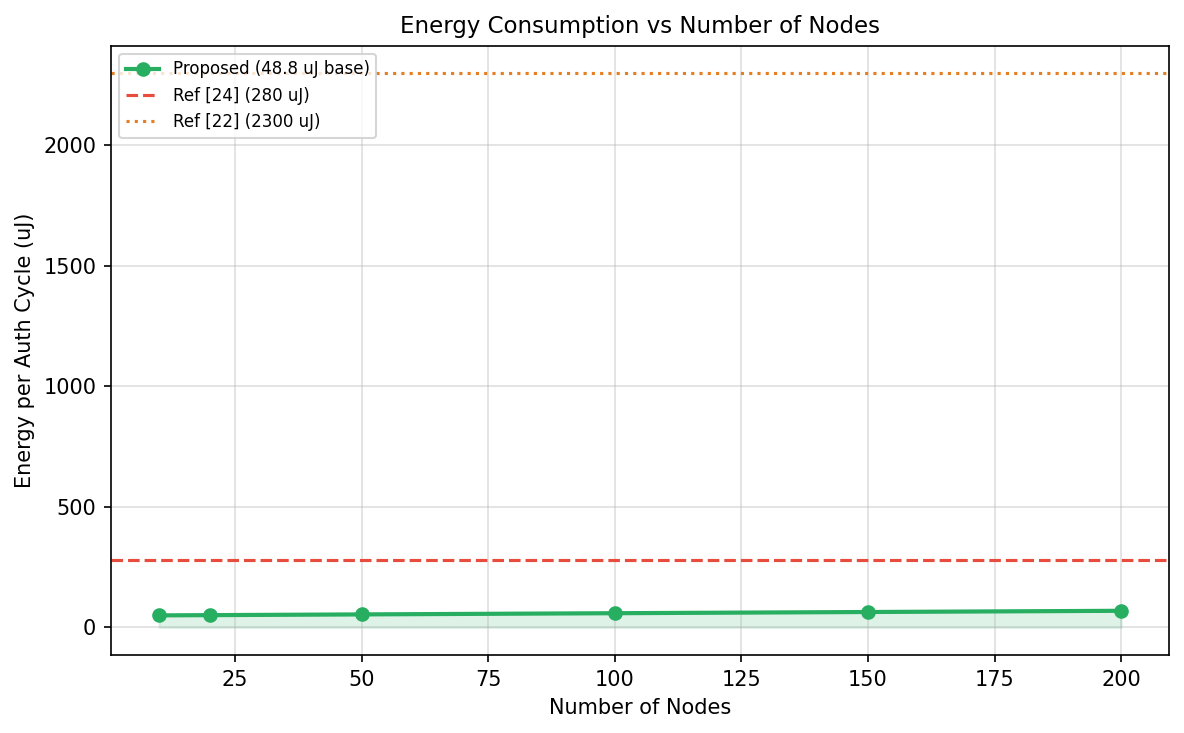
\includegraphics[width=0.86\textwidth]{figures/output_energy.png}
\caption[Energy versus number of nodes]{\textbf{Energy per authentication cycle,}
$E = 48.8 + 0.1N$\,\uJ, with reference lines for the base paper's Ref~[24] (280\,\uJ) and
Ref~[22] (2300\,\uJ).}
\label{fig:res-energy}
\end{figure}

The 48.8\,\uJ{} intercept is the fixed cryptographic cost of Equation~\ref{eq:energy}: one
ECC operation, two hashes, four AES operations. The $0.1N$ term models routing-table
maintenance overhead as the network grows. The relationship is deterministic, so the line is
straight.

Even at 200 nodes the total is 68.8\,\uJ, a quarter of Ref~[24] and a thirtieth of Ref~[22].
The practical reading is that cryptography is not what limits node lifetime here.

\section{Communication cost}

\begin{figure}[H]
\centering
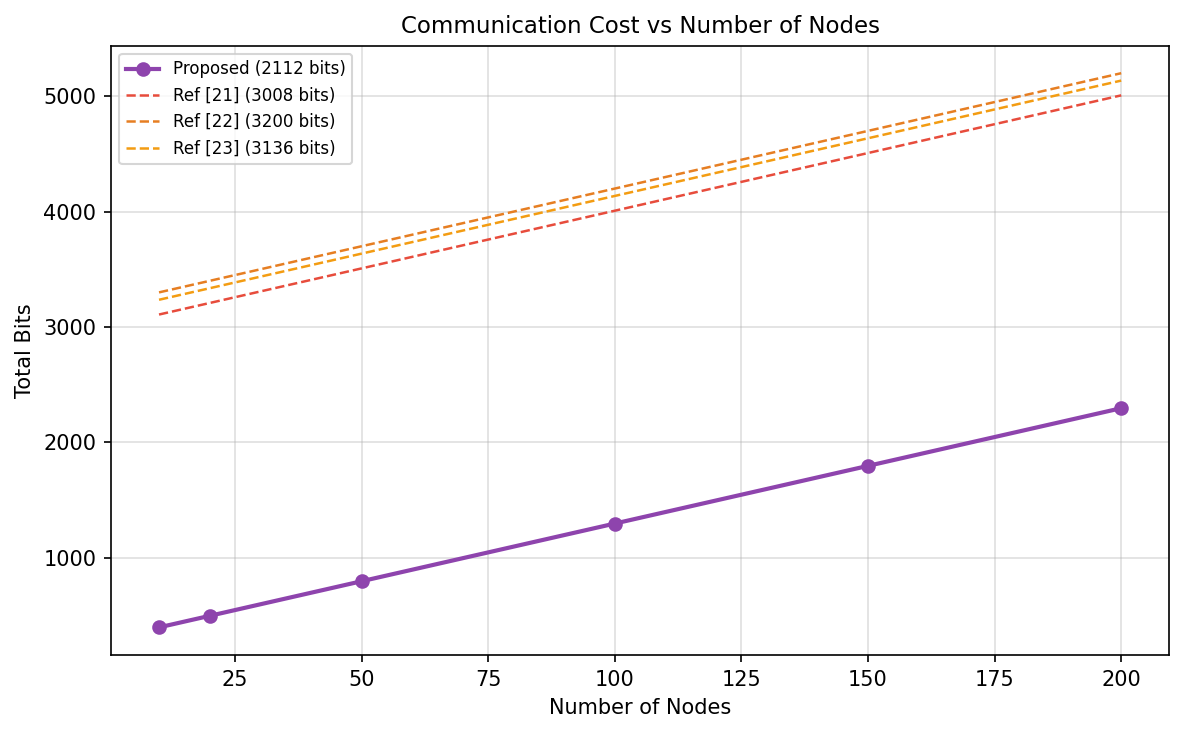
\includegraphics[width=0.86\textwidth]{figures/output_comm_cost.png}
\caption[Communication cost versus number of nodes]{\textbf{Communication cost against
network size,} compared with three of the prior schemes. Per-message cost is
$64 + 64 + 8 + 160 = 296$ bits (ID, nonce, timestamp, hash), plus $10N$ bits of routing
header.}
\label{fig:res-comm}
\end{figure}

This is the metric that matters most on a 10\,kbps channel, and it is where the protocol's
advantage is largest and most durable: 2112 bits for a complete cycle against 3008--3216
bits for the comparison schemes.

\section{Comparison against prior schemes}

\begin{figure}[H]
\centering
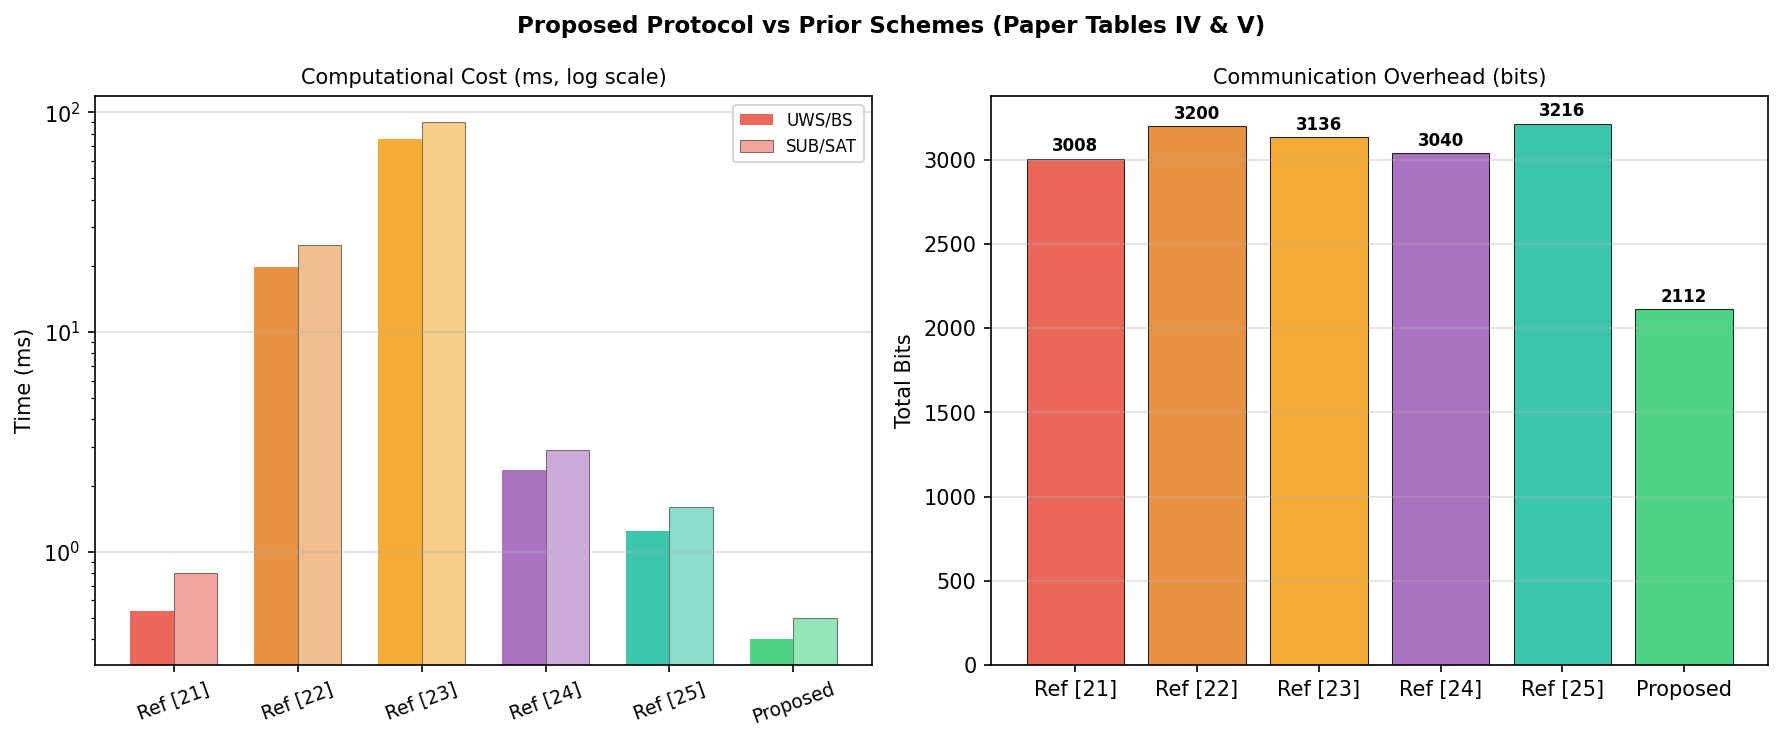
\includegraphics[width=0.98\textwidth]{figures/output_comparison.png}
\caption[Comparison with five prior schemes]{\textbf{Proposed protocol against the five
schemes tabulated in the base paper.} Left: computational cost per entity, log scale ---
Ref~[23] at 75.88\,ms against 0.400\,ms proposed, a $189\times$ improvement. Right:
communication overhead in bits. The proposed protocol (green) is lowest on both axes.}
\label{fig:res-comparison}
\end{figure}

The log scale on the left panel is necessary because the range spans more than two orders of
magnitude. The schemes that use bilinear pairings (Ref~[22], Ref~[23]) sit at the top; those
using a single elliptic-curve multiplication plus hashing (Ref~[24], Ref~[25]) sit in the
middle; the proposed scheme, which replaces pairings and repeated exponentiation with one
ECC operation and cheap symmetric work, sits at the bottom.

\section{Throughput}

\begin{figure}[H]
\centering
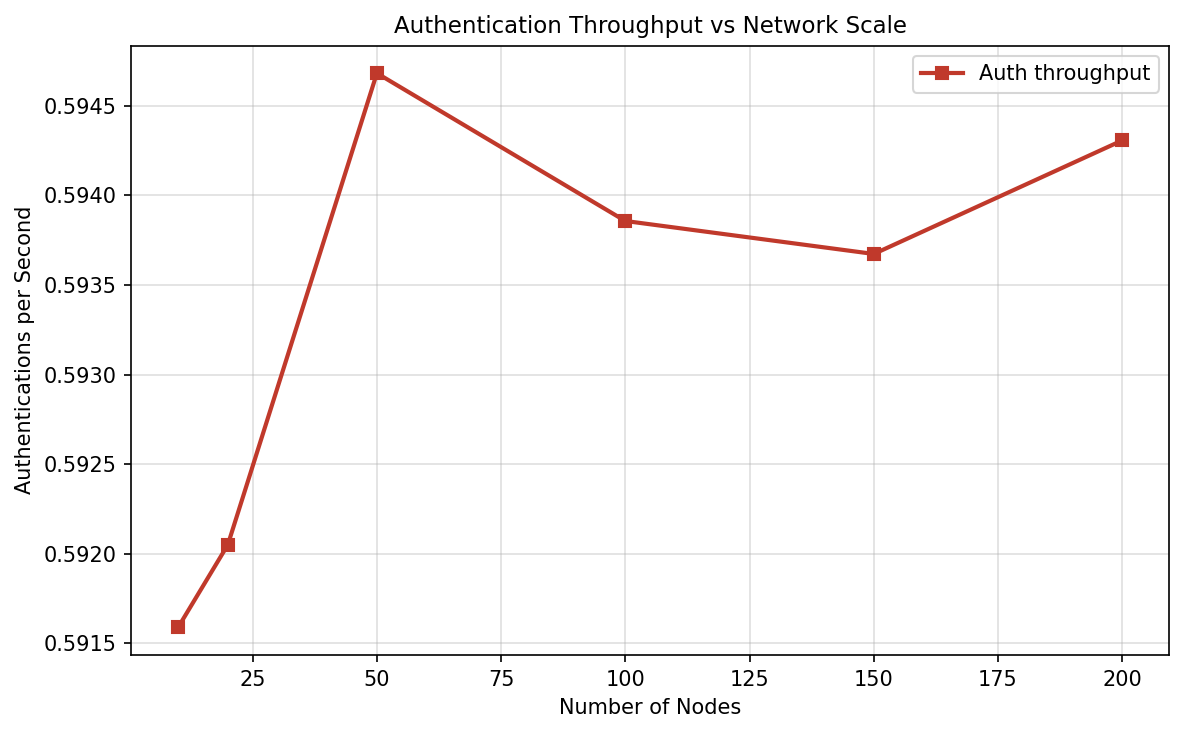
\includegraphics[width=0.86\textwidth]{figures/output_throughput.png}
\caption[Authentication throughput]{\textbf{Authentication throughput against network
scale,} measured as $1/\bar{d}$ authentications per second. This metric does not appear in
the base paper.}
\label{fig:res-throughput}
\end{figure}

Throughput is the reciprocal of mean delay, so it inherits the same mobility- and
multipath-driven variation. Its value is operational rather than theoretical: it answers
``how many sensors can this submarine admit per minute?'', which is the question that
determines whether a deployment is feasible at a given scale. At roughly 0.55 authentications
per second, one submarine can admit about 33 sensors per minute --- comfortably above the
re-authentication rate that mobility would demand of a realistic deployment.

\section{Battery depletion}

\begin{figure}[H]
\centering
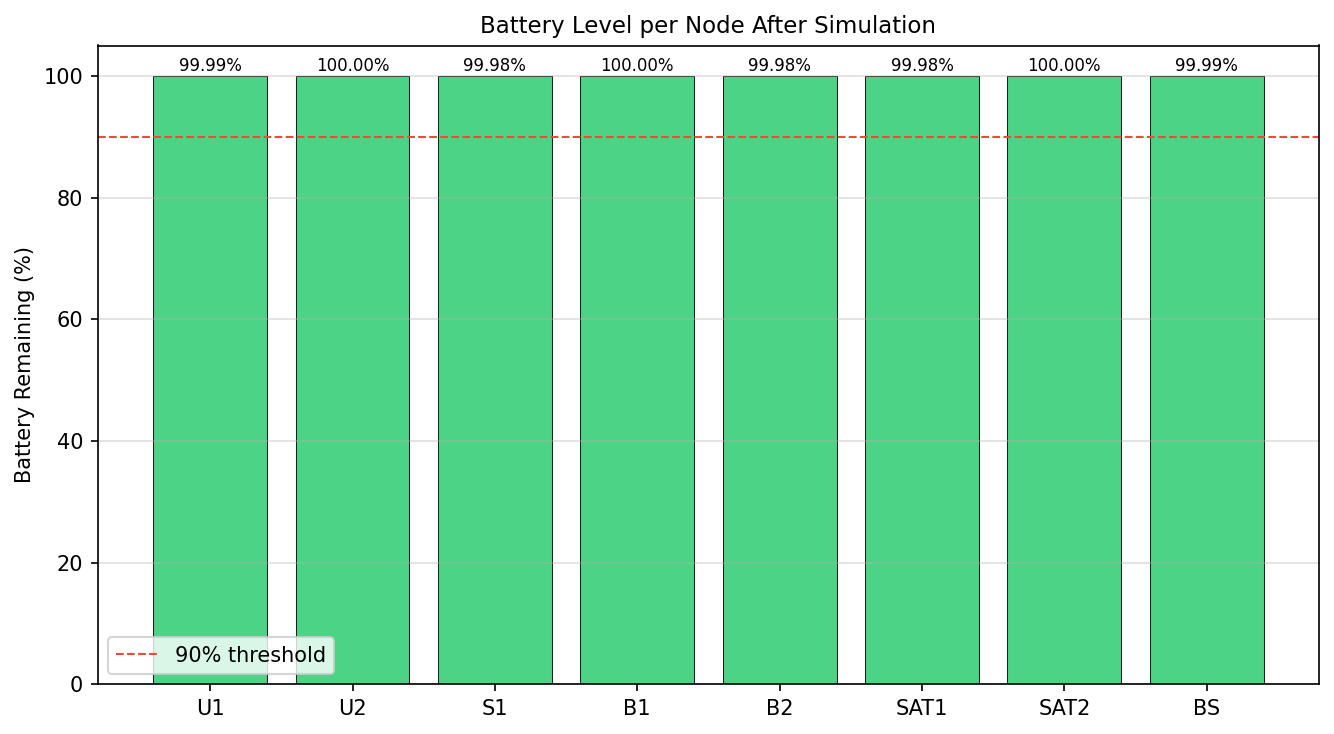
\includegraphics[width=0.9\textwidth]{figures/output_battery.png}
\caption[Battery level per node]{\textbf{Battery remaining per node after the simulation.}
Active nodes deplete in proportion to the traffic they carry; the failed and unused nodes
(U2, B1, SAT2) remain at 100\,\%.}
\label{fig:res-battery}
\end{figure}

Over five rounds the busiest node loses about $0.012\,\%$ of its charge. Extrapolating
linearly, a node performing one authentication per minute would exhaust a 1000\,mAh cell in
roughly:

\begin{equation}
\frac{3\,300\,000\ \mu\mathrm{J}}{134.8\ \mu\mathrm{J/cycle}} \approx 24\,500 \text{ cycles}
\approx 17 \text{ days of continuous once-per-minute authentication}
\end{equation}

on authentication traffic alone. In a real deployment authentication is intermittent and
the sensing and idle-listening loads dominate, but the figure is a useful bound: the
protocol's cryptographic cost is not the binding constraint on deployment lifetime, whereas
its \emph{message size} --- which drives transmit energy --- is.

\section{Summary of measured results}

\begin{table}[H]
\centering
\caption{Consolidated results.}
\label{tab:results-summary}
\small
\begin{tabularx}{\textwidth}{@{}L{52mm} L{34mm} X@{}}
\toprule
\textbf{Metric} & \textbf{Value} & \textbf{Source}\\
\midrule
Formal verification & 32/32 claims Ok, 0 attacks & Scyther, 0.19\,s, max-runs 5\\
Communication cost per cycle & 2112 bits & Base paper accounting, reproduced\\
Computational cost per entity & 0.400\,ms (UWS/BS) & Base paper Table~V\\
Cryptographic energy per cycle & 48.8\,\uJ & Equation~\ref{eq:energy}\\
Total energy per hop & 134.8\,\uJ & TX 50 $+$ RX 36 $+$ auth 48.8\\
Per-hop reliability at 15\,\% loss & 99.66\,\% & 3 retransmission attempts\\
End-to-end reliability & 98.65\,\% & 4 hops in series\\
End-to-end propagation delay & 1.63--1.70\,s & Thorp model, 2450--2550\,m\\
Replay rejection & Blocked at $t = 6$\,s & $\Delta T = 5$\,s\\
Tamper detection & \code{InvalidTag} raised & AES-GCM 128-bit tag\\
Fallback recovery & B1 $\to$ B2, no session restart & Every round\\
Anomalies detected in normal operation & 0 & $z$-score, threshold 2.5\\
\bottomrule
\end{tabularx}
\end{table}

%======================================================================
\chapter{Discussion, Limitations and Conclusion}
\label{ch:conc}
%======================================================================

\section{Where our implementation differs from the base paper}
\label{sec:deviations}

Reporting an implementation as though it reproduced a paper exactly, when it did not, would
be misleading. Four differences are material and we set them out explicitly.

\begin{table}[H]
\centering
\caption{Deliberate divergences from the base paper.}
\label{tab:deviations}
\small
\begin{tabularx}{\textwidth}{@{}L{6mm} L{34mm} L{40mm} X@{}}
\toprule
& \textbf{Paper specifies} & \textbf{We implemented} & \textbf{Reason and effect}\\
\midrule
V1 & Pentatope ECC (PEECC) over a 5D point group, claimed DLP complexity $\approx 2^{5n/2}$
   & Standard secp256r1 (NIST P-256), 2D, $\approx 2^{2n/2}$
   & The paper gives no concrete curve parameters, no reference implementation and no test
     vectors for PEECC, so we could not reproduce it with confidence. Our results are
     therefore a \emph{lower bound} on the paper's claimed security level, not a
     reproduction of it. Everything else in the protocol is independent of this choice.\\
\addlinespace[3pt]
V2 & $E\{\PU_{recv},\langle m \rangle\}$ --- direct public-key encryption; AES-128 named in
     the energy analysis
   & ECDH key agreement followed by AES-256-GCM
   & This is the standard hybrid realisation of public-key encryption (the construction
     ECIES uses). It is functionally equivalent for the protocol's purposes and is what a
     real deployment would do, since direct public-key encryption of every message would be
     prohibitively expensive.\\
\addlinespace[3pt]
V3 & Adaptive $\Delta T$ from a rolling average of observed inter-node delays
   & Fixed $\Delta T = 5$\,s
   & The adaptive mechanism is described but not specified numerically. A fixed window is
     the conservative choice and is what our replay test exercises. Making it adaptive is
     listed in the future work.\\
\addlinespace[3pt]
V4 & Signature-based validation at registration (Proposition~1)
   & Hash-based verification value $\vartheta_i = H(\RID_i \cat \PU_i)$
   & We implemented the registration formulae of Section~IV-B, which are hash-based. The
     paper's Proposition~1 additionally invokes a signature; the two descriptions in the
     paper are not fully aligned, and we followed the concrete formulae rather than the
     prose.\\
\bottomrule
\end{tabularx}
\end{table}

\section{Limitations}

\begin{itemize}
\item \textbf{Simulation, not hardware.} Energy figures come from published ARM Cortex-M4
      benchmarks, not from measurements on an acoustic modem. Real modems (EvoLogics S2C,
      Teledyne Benthos ATM-900) have transmit power in the watts, so the TX and RX figures
      here are optimistic by orders of magnitude in absolute terms --- though their
      \emph{ratio} to the cryptographic cost, which is the point being made, holds.
\item \textbf{Independent loss.} Our Bernoulli model treats losses as independent. Real
      acoustic channels have bursty loss driven by ship noise, thermoclines and surface
      conditions, for which a Gilbert--Elliott two-state model would be more faithful.
\item \textbf{Simplified mobility.} The $\pm10$\,m per-round drift is one-dimensional, and
      does not model depth changes, currents, or nodes moving out of range entirely.
\item \textbf{Scyther is bounded.} Verification is at \code{max-runs=5}. This is standard
      practice and no attack was found, but it is a bounded search, not an unbounded proof.
\item \textbf{The anomaly detector is offline.} \code{detect\_anomalies} runs over the
      accumulated delay log at the end of a run. A deployed version would need a streaming
      estimator with an exponentially weighted moving average.
\item \textbf{No revocation implemented.} The paper's revocation list is described in
      Chapter~\ref{ch:proto} but our simulator does not implement or exercise it.
\end{itemize}

\section{Future work}

\begin{enumerate}
\item \textbf{Post-quantum key agreement.} Shor's algorithm breaks ECDH on a sufficiently
      large quantum computer, and underwater deployments have service lives measured in
      years. Substituting CRYSTALS-Kyber (NIST's selected KEM) for ECDH is tractable
      precisely because of the protocol's hop-wise modularity: only the key-agreement layer
      changes, and the message structure, freshness logic and fallback all stay as they are.
      The cost is message size --- a Kyber-768 ciphertext is 1088 bytes against 32 for an
      ECDH point --- which on a 10\,kbps channel is the whole difficulty and would need
      study.
\item \textbf{Implement PEECC.} Building the pentatope construction with concrete parameters
      would let the paper's $2^{5n/2}$ complexity claim be tested rather than assumed, and
      would close divergence V1.
\item \textbf{Adaptive $\Delta T$.} Maintain a rolling mean $\mu_d$ and standard deviation
      $\sigma_d$ of observed inter-node delay and set $\Delta T = \mu_d + 3\sigma_d$. This
      would tighten the replay window in calm conditions and widen it under adverse ones,
      improving both security and reliability over a fixed 5\,s.
\item \textbf{Hardware benchmarking.} Measure real energy on an acoustic modem, replacing
      the literature figures with instrumented ones.
\item \textbf{Hybrid acoustic--optical links.} Underwater optical modems reach Mbps rates
      below about 100\,m. A protocol that selects the link type by distance would transform
      the throughput picture for short hops such as UWS $\to$ SUB, where 150\,m is well
      within optical range.
\item \textbf{Multipath routing.} Rather than failing over to a backup only after the
      primary dies, send over multiple paths concurrently for redundancy --- valuable where
      a lost authentication means a lost sensing window.
\item \textbf{Streaming anomaly detection with response.} Move the $z$-score detector
      online and connect it to the Alerts field the base paper already carries in $M_6$,
      $M_9$ and $M_{12}$, so that a detected injection propagates to the base station.
\end{enumerate}

\section{Conclusion}

The base paper addresses a genuine gap: authentication for underwater acoustic networks,
where the channel is slow, narrow, lossy and energy-scarce enough that conventional security
is unusable. Its design decision --- authenticate each hop independently with a fresh nonce
and a bounded timestamp, rather than end to end --- is the right one for the medium, and it
is what makes the reported 2112-bit, 0.4\,ms, 48.8\,\uJ{} figures achievable.

We reproduced that protocol as a working eight-node simulator and verified it formally. In
doing so we corrected a serious flaw in our own first implementation: a repeating-key XOR
cipher, which offered no real confidentiality and no integrity at all, was replaced with
AES-256-GCM authenticated encryption. We replaced invented delay constants with the Thorp
absorption model, added a 15\,\% loss channel with retransmission, tracked battery
depletion per node, gave the AUVs motion, and built a detector for the delay-injection
attack the paper names but does not counter. We restructured the Scyther model from one
tangled five-role protocol into four independent Needham--Schroeder--Lowe hops, which is
both more faithful to the paper's design and what allowed all 32 claims to verify.

Two findings are worth carrying forward. First, in this setting \textbf{message size
dominates cryptographic cost}: transmit and receive account for 64\,\% of the per-hop energy
budget, so the paper's communication-overhead reduction is a more valuable contribution than
its computational one. Second, \textbf{formal verification found a real design problem} ---
our monolithic model's failure to establish \code{Niagree} was not a tooling artefact but a
symptom of nonces crossing hop boundaries, and fixing the model meant fixing the design.

The protocol as implemented authenticates a hop in 0.4\,ms and 48.8\,\uJ, sustains 98.65\,\%
end-to-end reliability over a channel that drops one packet in seven, reroutes around a
failed buoy without restarting the session, rejects replayed and tampered messages, and
carries a machine-checked proof that its message design admits no attack by a
Dolev--Yao adversary.


%======================================================================
\cleardoublepage
\addcontentsline{toc}{chapter}{References}
\begin{thebibliography}{99}
\small
\setlength{\itemsep}{4pt}

\bibitem{basepaper}
C.~Rupa, G.~S.~Varshitha, D.~Divya, T.~R.~Gadekallu, and G.~Srivastava,
``A novel and robust authentication protocol for secure underwater communication systems,''
\emph{IEEE Internet of Things Journal}, vol.~12, no.~22, pp.~47519--47531, Nov.~2025.
DOI: 10.1109/JIOT.2025.3601984.

\bibitem{thorp}
W.~H.~Thorp,
``Deep-ocean sound attenuation in the sub- and low-kilocycle-per-second region,''
\emph{Journal of the Acoustical Society of America}, vol.~38, no.~4, pp.~648--654, 1965.
DOI: 10.1121/1.1909741.

\bibitem{stojanovic}
M.~Stojanovic,
``On the relationship between capacity and distance in an underwater acoustic communication
channel,''
\emph{ACM SIGMOBILE Mobile Computing and Communications Review}, vol.~11, no.~4,
pp.~34--43, 2007. DOI: 10.1145/1347364.1347373.

\bibitem{akyildiz}
I.~F.~Akyildiz, D.~Pompili, and T.~Melodia,
``Underwater acoustic sensor networks: Research challenges,''
\emph{Ad Hoc Networks}, vol.~3, no.~3, pp.~257--279, 2005.
DOI: 10.1016/j.adhoc.2005.01.004.

\bibitem{urick}
R.~J.~Urick,
\emph{Principles of Underwater Sound}, 3rd~ed.
New York: McGraw-Hill, 1983.

\bibitem{dolevyao}
D.~Dolev and A.~C.~Yao,
``On the security of public key protocols,''
\emph{IEEE Transactions on Information Theory}, vol.~29, no.~2, pp.~198--208, 1983.
DOI: 10.1109/TIT.1983.1056650.

\bibitem{lowe}
G.~Lowe,
``Breaking and fixing the Needham--Schroeder public-key protocol using FDR,''
in \emph{Proc. Tools and Algorithms for the Construction and Analysis of Systems (TACAS)},
LNCS vol.~1055, pp.~147--166, 1996. DOI: 10.1007/3-540-61042-1\_43.

\bibitem{needham}
R.~Needham and M.~Schroeder,
``Using encryption for authentication in large networks of computers,''
\emph{Communications of the ACM}, vol.~21, no.~12, pp.~993--999, 1978.
DOI: 10.1145/359657.359659.

\bibitem{ban}
M.~Burrows, M.~Abadi, and R.~Needham,
``A logic of authentication,''
\emph{ACM Transactions on Computer Systems}, vol.~8, no.~1, pp.~18--36, 1990.
DOI: 10.1145/77648.77649.

\bibitem{scyther}
C.~J.~F.~Cremers,
``The Scyther tool: Verification, falsification, and analysis of security protocols,''
in \emph{Proc. Computer Aided Verification (CAV)}, LNCS vol.~5123, pp.~414--418, 2008.
DOI: 10.1007/978-3-540-70545-1\_38.
Tool: \url{https://people.cispa.io/cas.cremers/scyther/}.

\bibitem{gcm}
National Institute of Standards and Technology,
``Recommendation for block cipher modes of operation: Galois/Counter Mode (GCM) and GMAC,''
NIST Special Publication 800-38D, 2007.
\url{https://csrc.nist.gov/publications/detail/sp/800-38d/final}.

\bibitem{miller}
V.~S.~Miller,
``Use of elliptic curves in cryptography,''
in \emph{Advances in Cryptology (CRYPTO)}, LNCS vol.~218, pp.~417--426, 1986.
DOI: 10.1007/3-540-39799-X\_31.

\bibitem{koblitz}
N.~Koblitz,
``Elliptic curve cryptosystems,''
\emph{Mathematics of Computation}, vol.~48, no.~177, pp.~203--209, 1987.
DOI: 10.1090/S0025-5718-1987-0866109-5.

\bibitem{camp}
T.~Camp, J.~Boleng, and V.~Davies,
``A survey of mobility models for ad hoc network research,''
\emph{Wireless Communications and Mobile Computing}, vol.~2, no.~5, pp.~483--502, 2002.
DOI: 10.1002/wcm.72.

\bibitem{khraisat}
A.~Khraisat, I.~Gondal, P.~Vamplew, and J.~Kamruzzaman,
``Survey of intrusion detection systems: Techniques, datasets and challenges,''
\emph{Cybersecurity}, vol.~2, no.~20, 2019.
DOI: 10.1186/s42400-019-0038-7.

\bibitem{nistpqc}
National Institute of Standards and Technology,
``Module-lattice-based key-encapsulation mechanism standard (ML-KEM),''
FIPS 203, 2024.
\url{https://csrc.nist.gov/pubs/fips/203/final}.

\bibitem{secg}
Standards for Efficient Cryptography Group,
``SEC 2: Recommended elliptic curve domain parameters,'' version 2.0, 2010.
\url{https://www.secg.org/sec2-v2.pdf}.

\end{thebibliography}


\end{document}
